% University of Leeds PhD thesis style -- modifications to the report style
% This is unofficial so you should always double check against the
% Registrar's office rules
% See http://library.stanford.edu/research/bibliography-management/latex-and-bibtex
% 
% Example of use below
% See the suthesis-2e.sty file for documentation
%
\documentclass{report}
\usepackage{suthesis-2e}
\dept{Electronic and Electrical Engineering}

\usepackage{hyperref}
\usepackage{graphicx}
\usepackage{color,soul}
\usepackage{listings}
\usepackage{xcolor}
\usepackage{xeCJK}
\usepackage{pdfpages,caption}
\usepackage[final]{pdfpages}

\begin{document}
\title{CENTRALISED CONTROL ALGORITHMS FOR SMART GRID OPERATION}
\author{Jialeng Guo}
%\principaladviser{John Parker}
%\firstreader{John Green}
%\secondreader{John BigBooty}
%\thirdreader{Jane Supernumerary} %if needed
%\fourthreader{Severus Snape} %if needed

\beforepreface
\prefacesection{Abstract}
Maintaining the frequency at the nominal value in the grid is one of the most elusive and long-standing challenges in smart grids. This project tackles the problem of frequency changes: how to design an algorithm to build a centralised Secondary Frequency Control (SFC) and to analyse the performance of the gird. On the one hand, we think that our SFC algorithm can maintain the frequency. On the other hand, we would need an efficient and concise strategy to analyse the performance of the system if we want to build an optimal controller to ensure that the frequency of the electricity network is always restored to its nominal value when disturbances occur in the system.\\

In this project, we focus on PI Control: the most common control algorithm by far and the standard algorithm in SFC. Compared to traditional grids without SFC, this algorithm has proven to be more effective in maintaining the frequency.\\

This project consists of two parts. In the first part, we aim to understand the physical theory behind SFC and PI control and present our efforts at building effective SFC models.\\

In the second part of this project, we test our algorithm in RAMSES\textcolor{red}{\footnote{RAMSES is a time-domain dynamic simulator for future electric power systems. RAMSES document: https://ramses.paristidou.info}} based on Nordic Grid scenario. In particular, 1) how we test our system in a low time delay; 2) how we analyse the impact of different time delays; 3) how we analyse the impact of generator size and 4) how we test Emergency Control and analyse the impact of time delays.\\

\prefacesection{Acknowledgments}
A special thank to my supervisor Dr Petros Aristidou. He always has a very insightful, high-level view about the field while he is also uncommonly detail oriented and understands the nature of the problems very well. More importantly, Dr Aristidou is an extremely caring and supportive supervisor that I could not have asked for more.\\

Collaboration is a big lesson that I learned, and also a precious part of my undergraduate stage. I thank Sultan Alghamdi. He never reserved his minds when I tried to seek his help. I am glad that my research can help part of his doctoral subject. It was a very unique and rewarding experience for me.\\

I would like to thank Dr Zoran Ikonic. His passionate lecture (ELEC2540 Control Systems) and impressive experiment last year depended my understanding of PI control.\\

I would like thank Walter Roberson from MATLAB for helping me find the clue to solve the problem with plotting a 3D triangle surface plot without a clearly relationship between variables.\\

Lastly, I would like to thank other staffs and my fellow schoolmates in School of Electronic and Electrical Engineering, without them, this project would not be finished smoothly: Anna de Jong, Nathan Smith, Zikang Qian and Al Dabashi.\\



\afterpreface


\chapter{Introduction}
\section{Motivation} %1.1
The motivation for doing this project contains a vision of restructuring and sustainability of energy in the future.
\subsection{Problems in the Grid}
\subsubsection{A. Energy Crisis}
The energy crisis is one of the most essential and critical crises in the 21st century.

Nowadays, non-renewable resource still consists of a large proportion in the energy system. Non-renewable resource, or finite resource, is depleting. Although we might not meet the complete depletion of non-renewable resources in the future 50 years, based on Hotelling’s "Economics of Exhaustible Resources", David Ricardo proposed that as the historical production stock accumulates, higher grade ores get depleted and the producer resorts to lower grade ores, sustaining greater extraction costs. It means, the extraction costs will rise, and the price of the products based on ores will rise. Thus, we can assume that the price of most of the non-renewable resources, like oil, coal and gas, will rise since these have similar properties with ores.\\

\subsubsection{B. Climate Change}
According to the paper from Nature, climate change happened in the past 70 years. It has already had effects on the environment around us. Glaciers are shrinking and ices are breaking up earlier on lakes and rivers. Most climate scientists agree with that it is the human expansion that causes the global warming. As we know, carbon dioxide (CO2) is a significant component of the atmosphere.Atmospheric CO2 concentration has been increased by more than a third since the Industrial Revolution began. More importantly, atmospheric carbon dioxide has exceeded the highest level in the past 400,000 years.\\

\begin{figure}[htbp]
\centering
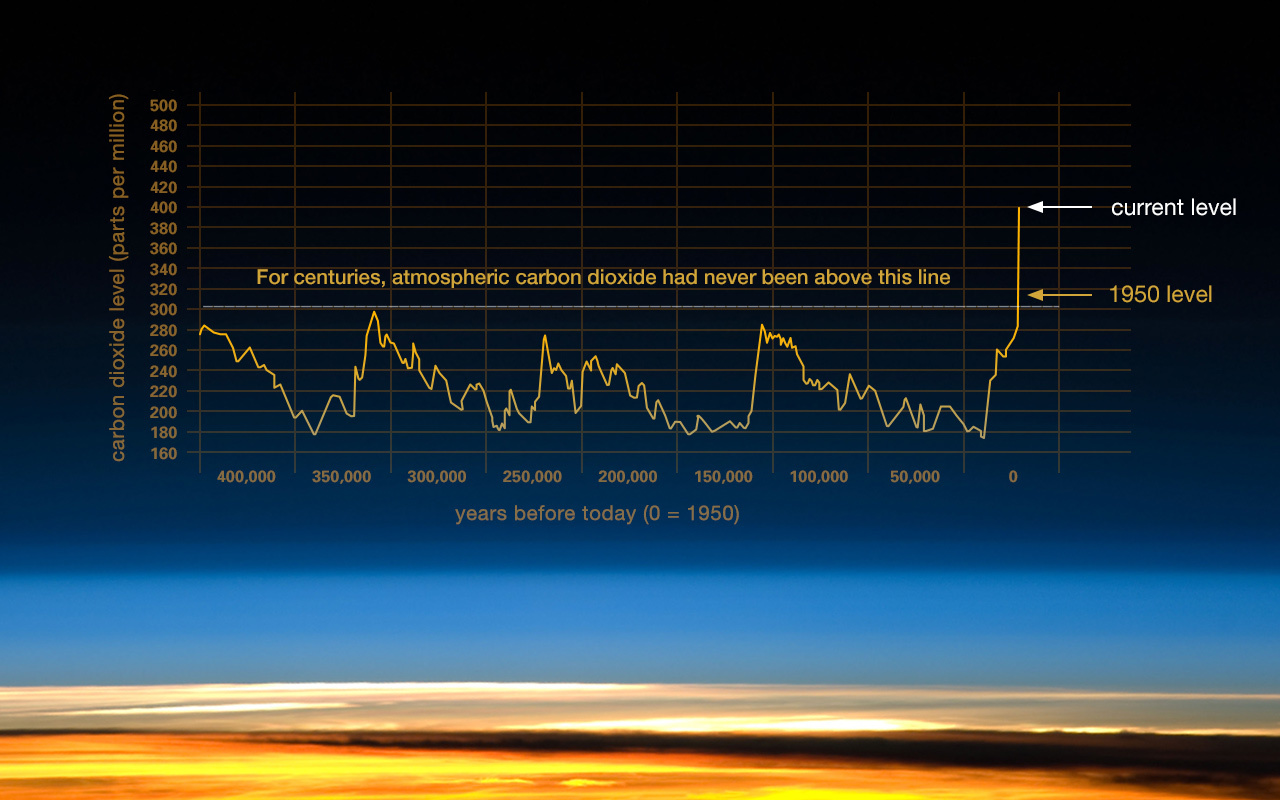
\includegraphics[width = \textwidth]{figure/1_1_1_nasa_co2.jpeg}
\caption{The evidence that atmospheric CO2 has increased since the Industrial Revolution began. Image courtesy: https://climate.nasa.gov/evidence/}
\label{1_1_1_nasa_co2}
\end{figure}

\subsubsection{C. Conflicts and Wars}
An unbalanced energy distribution causes conflicts and wars. The wars, like Gulf War, are more or less derived from energy issues since WW2.\\

\subsubsection{D. Power Interruption}
With the use of unreliable electrical grids, power interruption occurs especially when a natural disaster, such as typhoon, earthquake, and wildfire, happens. Smart grids is more reliable than traditional grids. It’s possible to be build a dynamic technology, like Secondary Frequency Control (SFC), that grid operators need. Self-healing is possible when the storms hit, or physical attack occurs. Therefore, consumers will not encounter power interruptions.\\

\subsubsection{E. Equal Rights to Use Natural Power}
Everyone should have his/her right to use natural resources equally. However, in most countries, the fact is that a few large companies occupy the dominant position of public funds and gradually form a monopoly market. Entrepreneurs use their centralised power to restrict consumers’ right to disagree.\\

However, the technologies should start with the customers. It is connected with intelligent devices that always communicate with each other. The system creates and stores energy throughout the day and any extra energy flows back onto the grid to power neighbours and businesses. Those smart energy buildings then power entire communities. It’s distributed, clean, and more cost-effective.\\

\subsubsection{F. New Issues from Clean Energy}
Using clean energy from renewable resource could be one of the ways to solve the problems above! In fact, recently, California Assembly passed a bill requiring 100 percent of the state’s electricity to come from carbon-free sources by the end of 2045. In China and Germany, renewables are outgrowing their grids. The public is accepting the idea of using electric cars instead of fuel cars.\\

However, these renewable energy sources interfaced with national or state power systems will introduce new issues on stability, resilience, and reliability. Thus, power networks are under modification.\\

For countries like Switzerland, where 62\% of electricity comes from renewable sources, it’s another situation. Although it’s really friendly to the environment, energy instability has also increased. Sun doesn’t always shine, wind doesn’t always blow, and water doesn’t always flow.\\

\subsection{Solution: Secondary Frequency Control}
As these highly variable sources come to represent a growing portion of the grid, it becomes more and more important to develop an accurate and validated model to represent these units in the computational tools used to analyse the ancillary services of smart grids.\\

Smart grids will power the modern city, and Secondary Frequency Control is one of the most important parts in smart grids to ensure the energy security in electricity systems and to allow increasing renewable energy penetration\\

Secondary Frequency Control ensures that the frequency of the electricity network is always restored to its nominal value when disturbances occur in the system. The frequency is one of the key “health” indicators of smart grids. Actively monitoring and controlling it will ensure system security. This is done by remotely controlling the power output of generating units (both conventional and renewables) through a communication network.\\


\section{Thesis Outline} %1.2
This project consists of two parts — PART I Algorithm and PART II Test Case Scenario (Nordic).\\

PART I focuses on the task of understanding and building Secondary Frequency Control (SFC) model and PI control algorithm so that we are able to test our cases in PART II.\\


In Chapter \textcolor{red}{\ref{Chapter2}}, we give an overview of Frequency Control, including Primary Frequency Control (PFC), Secondary Frequency Control (SFC) and Tertiary Frequency Control (TFC). We discuss the emergency control with PFC, SFC and TFC.\\

In Chapter \textcolor{red}{\ref{Chapter3}}, we formally focus on the physical theory behind Secondary Frequency Control (SFC) which is the base of the whole project. We briefly discuss PID control and argue that we should use PI control to reduce the probability of risk. We then discuss how to build a communication layer on top of an existing smart grid simulator and design a centralised controller for stabilising the system. We describe the algorithm we built named sfc: its key parameters, tuning methodology, and some implementations. We finally define the acceptable results based on the official report from Nordic, and with that, we build our own analytical tools. With these tools, we can plot a 2D even a 3D diagram, find the eligible results and give feedback to our controller in PART II.\\

PART II views testing in a specific test case scenario (Nordic) as an important part such as the impact of different time delays. Detailedly,\\

In Chapter \textcolor{red}{\ref{Chapter4}}, we focus on testing the system in a low time delay. We discuss how to choose an appropriate generator as a breaker and how to tune the range of  gain. Before simulating, we predict some expected results based on the physical theory behind Secondary Frequency Control (SFC). Then we present a comprehensive evaluation on the simulation results. We describe the results and compare them with the expected one. We discuss why my prediction had deviation or missing. We discuss the risk, i.e. the rate of change of power, of the generators and how to remove unacceptable results. We will finally show a 2d plot and a simulation result.\\

In Chapter \textcolor{red}{\ref{Chapter5}}, we discuss the impact of different time delays. We increase the delay and use the range of gain in Chapter 4. We will explain why we think it is reasonable to continue using the range of gain in Chapter 4. In fact, it is logical forward-looking. Then we will predict the simulation results based on the physical theory behind Secondary Frequency Control (SFC) and the results in Chapter 4. Then we present a comprehensive evaluation on the complicated simulation results. We will describe the results with a plotted 3d graph. We will discuss some unpredictable results and some seemingly irregular data. We discuss the risk of the generators, like what we do in Chapter 4, and how to remove unacceptable results. We will finally show a 3d plot and a best simulation result.\\

In Chapter \textcolor{red}{\ref{Chapter6}}, we discuss the impact of generator size. We fix the size of gain and the size of  delay in this chapter and we discuss the reason for doing this. Differently, We only test g1, g3, g4, g5, g9, g10, g11, g12, g13 and g19 as breaker, the generator will disconnected from the grid as the only disturbing factor, based on Section 4.1.1. Before implementing, we predict some expected results based on Section 4.1.1 and understanding on energy and power. We analyse the results and they prove our prediction. We will see the relationship between the output and the size of a generator. We finally analyse if the system will have risk and the relationship between the size of a generator and the chance to have a risk. \\

In Chapter \textcolor{red}{\ref{Chapter7}}, we test Emergency Control and discuss the impact of different time delays without tuning gains. We will firstly define Emergency Control although we have discussed it in Chapter 2. We predict some results based on Secondary Frequency Control (SFC) and the conclusions in Chapter 4. After implementing and analysing the results, we will discuss why my predictions are “wrong”. We finally do a risk assessment for the system as we did before.\\

We will finally conclude in Chapter \textcolor{red}{\ref{Chapter8}}.\\

\section{Contributions} %1.3
The contributions of this thesis are summarised as follows:\\
\begin{itemize}
  \item I built a communication layer on top of an existing Smart Grid simulator and design a centralised controller for stabilising the system.\\
  
  \item I researched situations that cause disturbances, including generators interruption, high time delays and blackout. We built a series of efficient models for analysing the performance of the system and remove any unacceptable results. After hundreds of manual data proofreading, these models has demonstrated superior analytical ability.\\
  
  \item I built an optimal controller for stabilising the frequency based on the centralised controller and the analytical models above. This optimal controller has demonstrated superior performance of restoring frequency when disturbances occur in the system.\\
  
  \item I learnt other important skills: test-driven development in Python, code modularity and collaborative version control.\\
\end{itemize}


\part{Algorithm}
\chapter{An Overview of Frequency Control}
\label{Chapter2}
\section{Overview} %2.1
Every country has its nominal frequency of the oscillations of alternating current in an electric power grid transmitted from a power station to the end-user. For instance, the nominal value is 50Hz in the UK while it’s 60Hz in USA.\\

However, if a load is suddenly connected or disconnected to the system, or if the protection equipment suddenly disconnects a generating, there will be a distortion in the power balance between that delivered by the turbines and that consumed by the loads. This imbalance is initially covered from the kinetic energy of rotating rotors of turbines, generators and motors and, as a result, the frequency in the system will change. \\

If there is a mismatch between the generation and the demand, for instance, due to the outage of one generating unit, then the frequency starts to drop down. \\

If no control is applied, the frequency largely deviates and then reaches a meagre and steady-state value, due to which the electrical grid is shut down.\\

\begin{figure}[htbp]
\centering
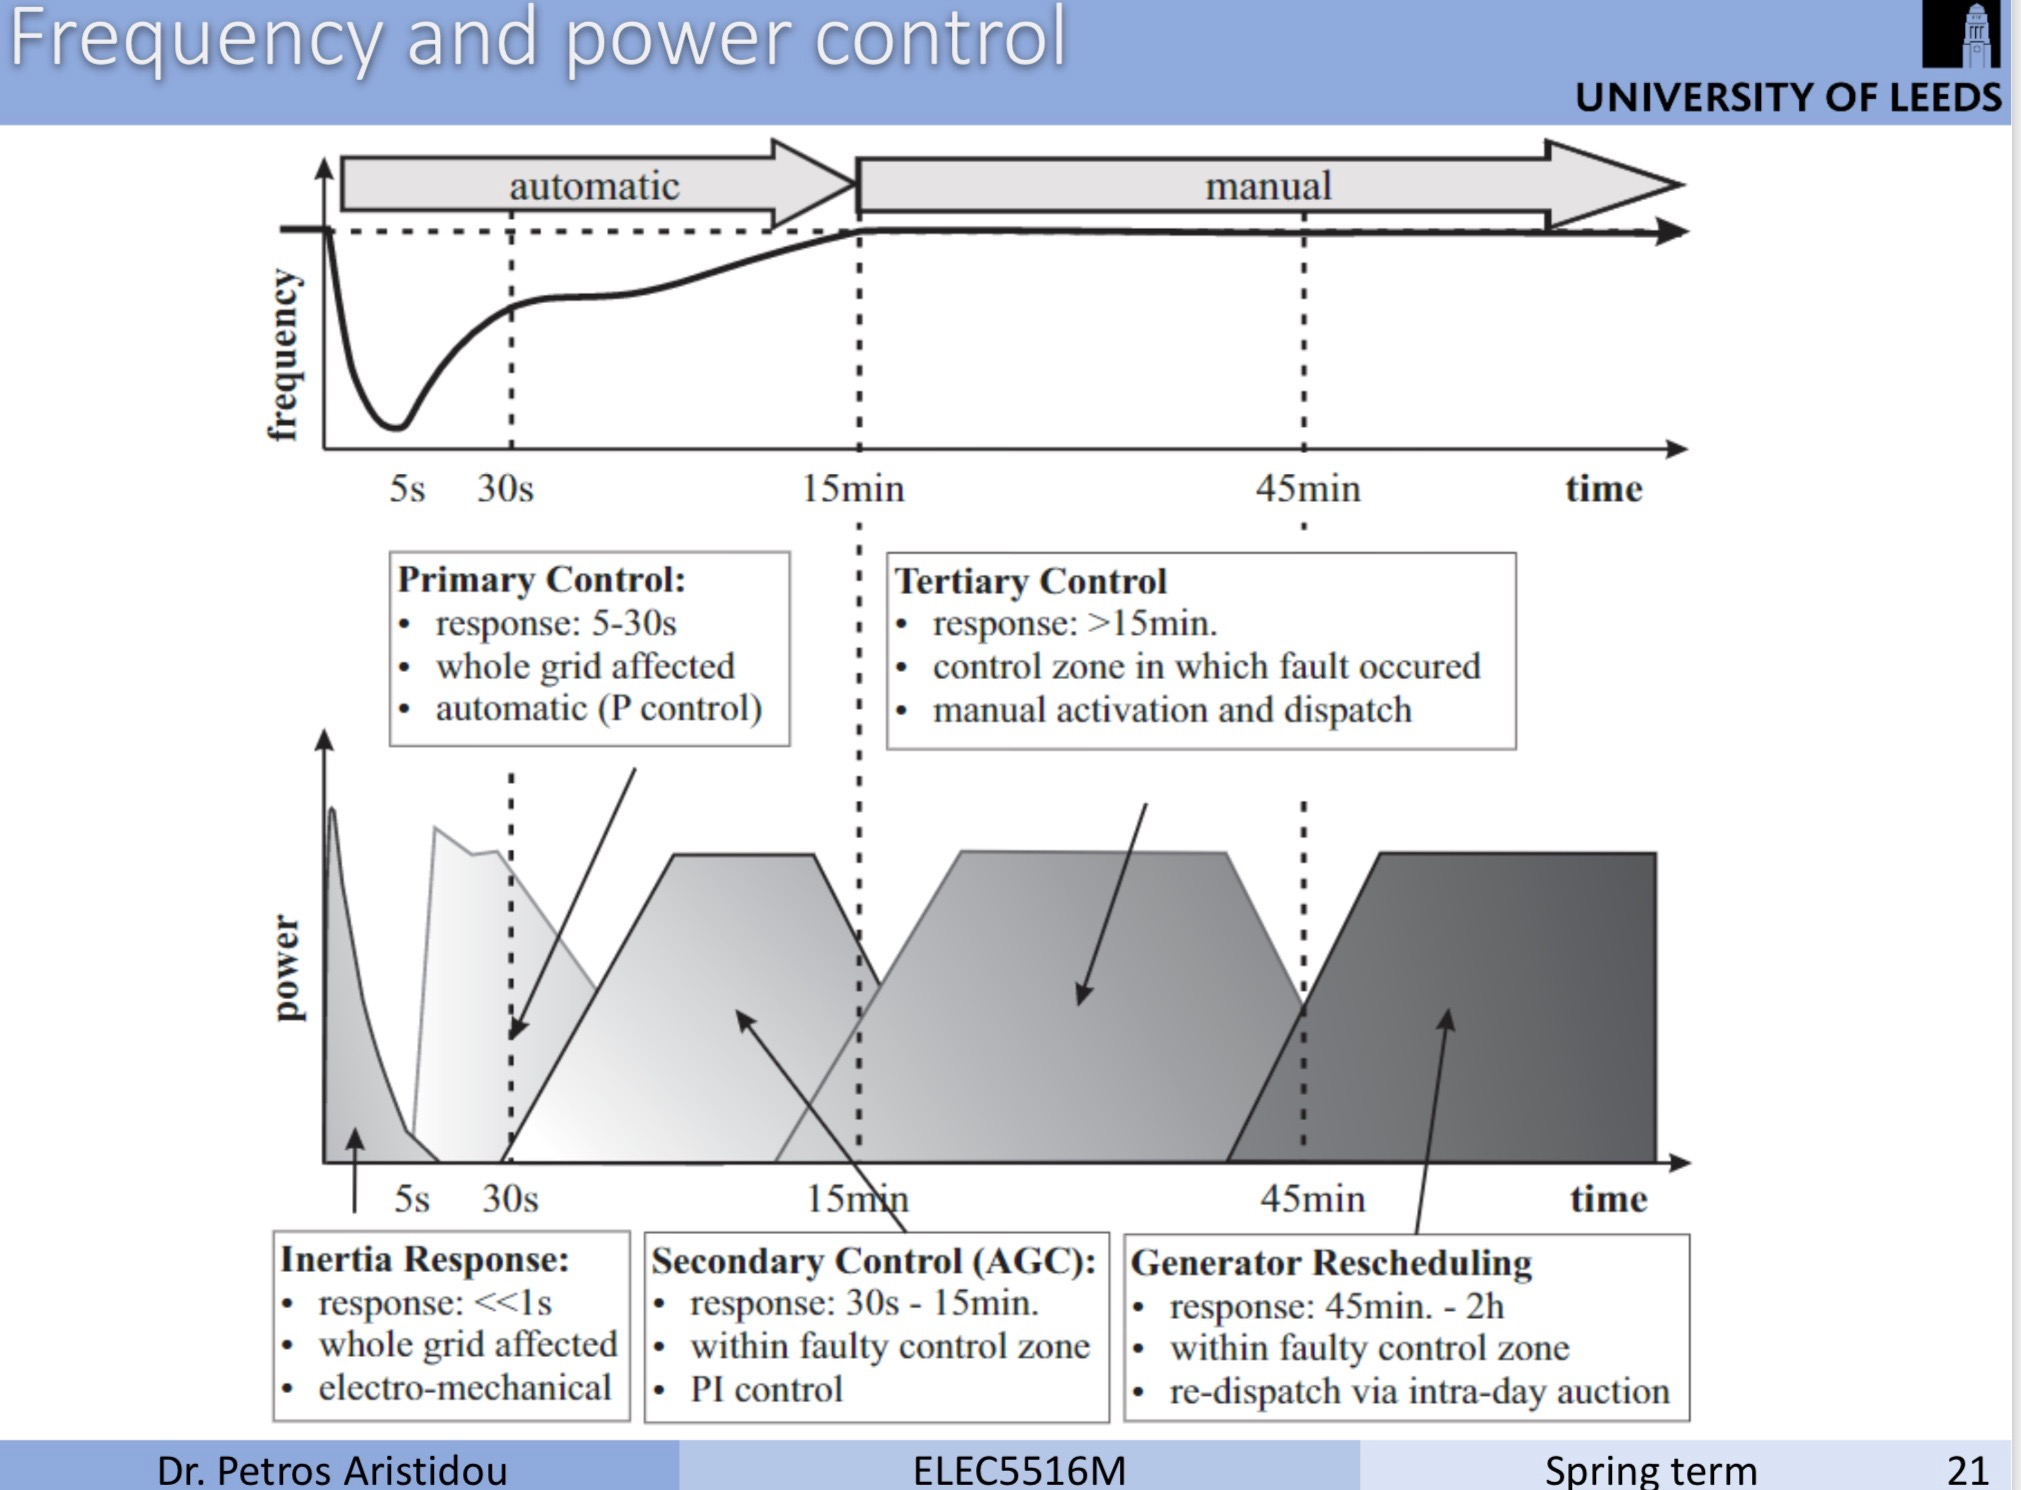
\includegraphics[width = \textwidth]{figure/2_1_freq.jpeg}
\caption{Frequency and power control}
\label{2_1_freq}
\end{figure}

The mechanism of primary frequency control is to restore the active power balance in a power system. After primary control takes place, the power balance is restored at a lower or higher frequency. Normally it takes seconds and responses from 5 seconds to 30 seconds. It is a partly Automatic Generation Control.\\


However, the frequency does not go back to its nominal value and remains at a steady-state value below or above the nominal one. To avoid damages to equipment and loads, we need secondary frequency control to restore the frequency balance to its nominal value or to eliminate the steady-state error/frequency error. Normally it takes minutes and responses from 30 seconds to 15 minutes. It is a fully Automatic Generation Control.\\


Tertiary Frequency Control encompasses actions taken to capture current and future emergencies by getting resources. Alternate deployment and recovery after a disturbance are common types of Tertiary Control. Normally it takes dozens of minutes and responses longer than 15 minutes. It is a fully manual control.



\chapter{PID Control Algorithm}
\label{Chapter3}
\section{The physical theory behind Secondary Frequency Control} %3.1
From Chapter \textcolor{red}{\ref{Chapter2}}, we mentioned that disturbances occur in the system, there will be a distortion in the power balance between that delivered by the turbines and that consumed by the loads. The imbalance is from the kinetic energy of rotating rotors of turbines, generators and motors and, thus, the frequency in the system will change. If no control is applied, the frequency largely deviates and then reaches a meagre and steady-state value, due to which the electrical grid is shut down. \\

We also mentioned that the system will firstly starts Primary Frequency Control and the frequency will remains at a steady-state value below or above the nominal one. After that, Secondary Frequency Control starts.\\

The mechanism of Secondary Frequency Control is to restore the frequency to the nominal one.\\

Secondary frequency control, or load frequency control (LFC), or automatic generation control (AGC), is an automatic control that restores the frequency back to its nominal value in a centralised way. It's implemented that is activated after the primary frequency control. Typically, it takes 30 seconds to 15 minutes.\\

\begin{figure*}[htbp]
\centering
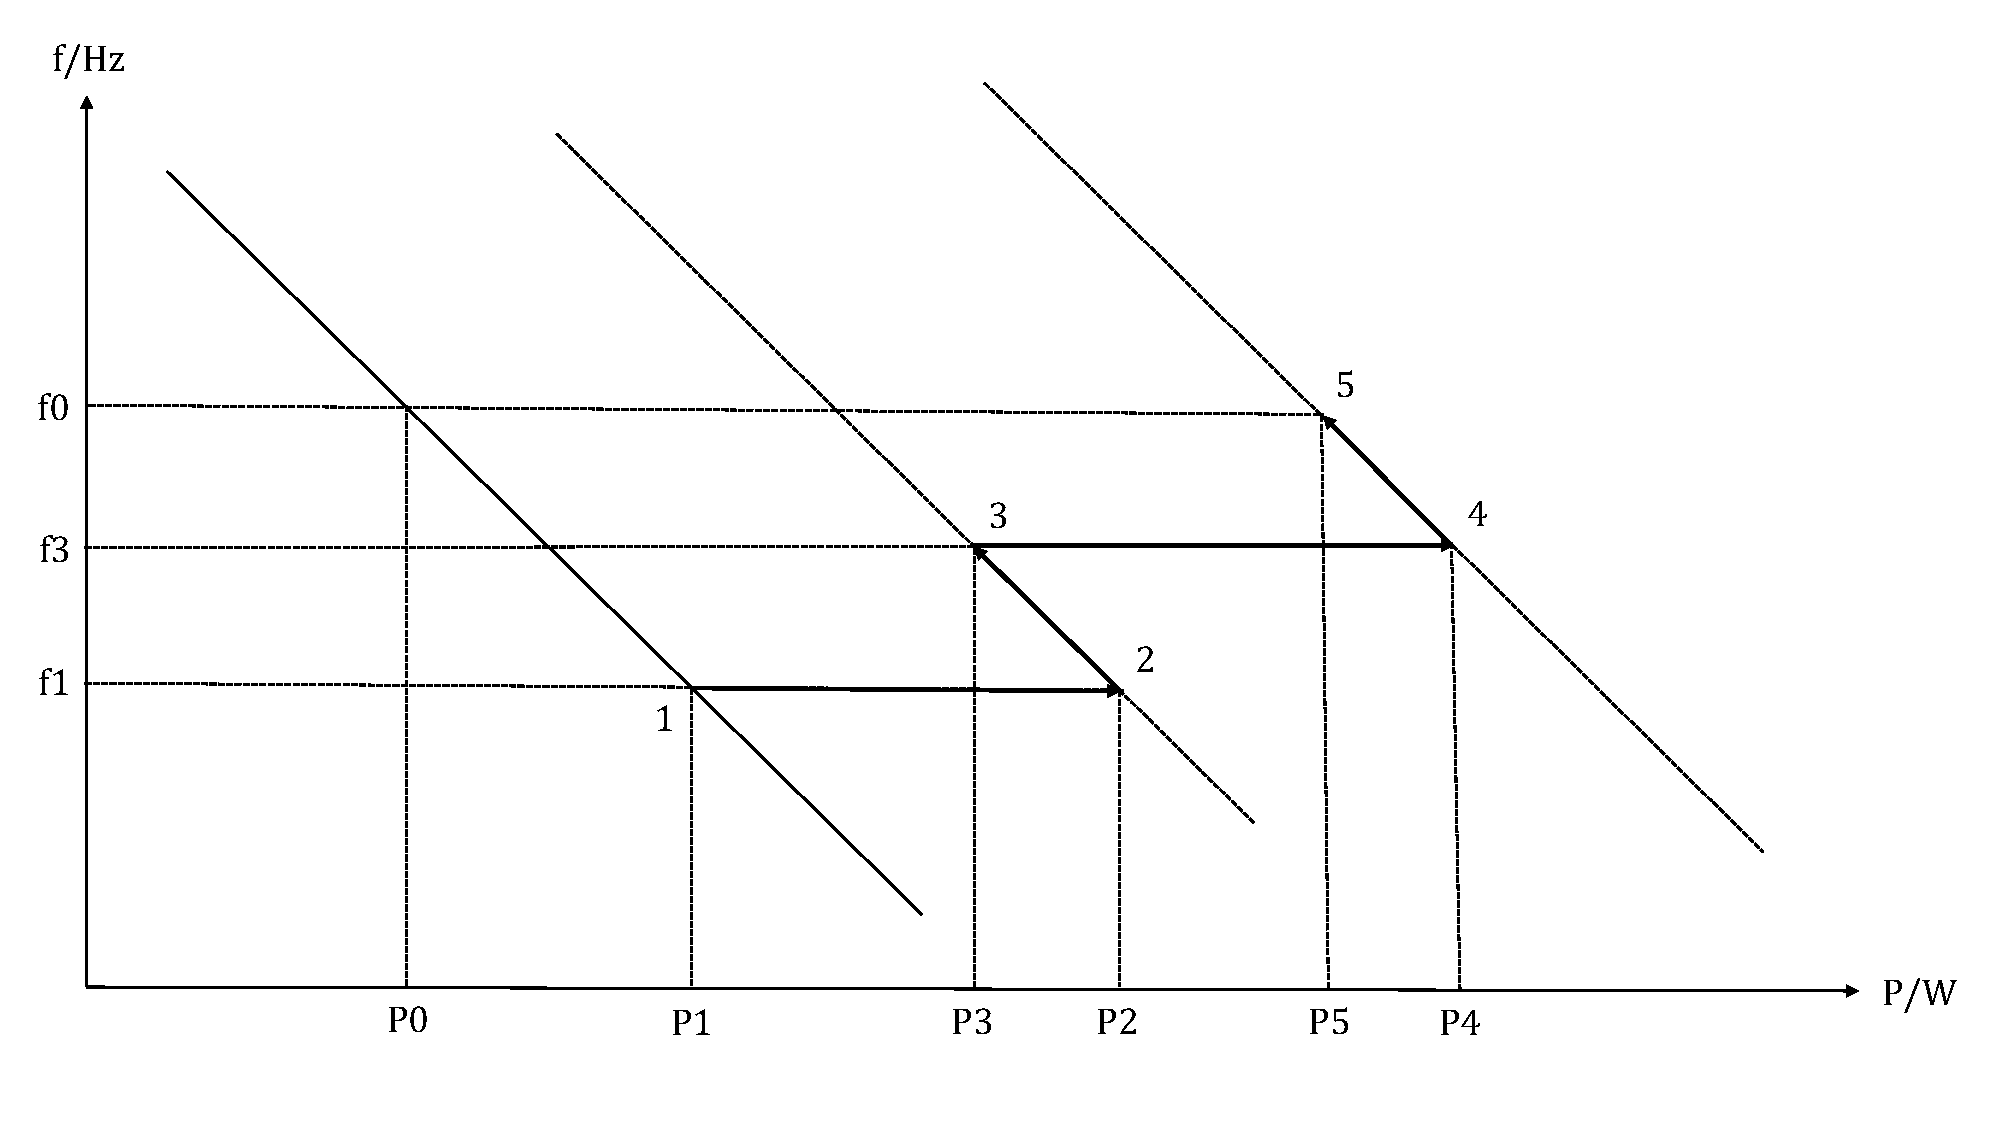
\includegraphics[width = \textwidth]{figure/3_1_Equilibrium.pdf}
\caption{Equilibrium points for an increase in the power demand.}
\label{3_1_Equilibrium}
\end{figure*}

According to Figure \textcolor{red}{\ref{3_1_Equilibrium}}, frequency value will rise as reference power rises. Assumed that point 1 is the situation after primary frequency control happens and point 5 has the nominal value of frequency. When trying to raise the reference power a little bit, point 1 will shift to point 2. Due to the power rise, the frequency of the system will rise, so point 2 will move to point 3. Changing more reference power of individual governors will move the overall generation characteristic of the system upwards. Eventually, this will lead to the restoration of the rated frequency ($f0$).\\

\begin{figure}[htb]
\centering
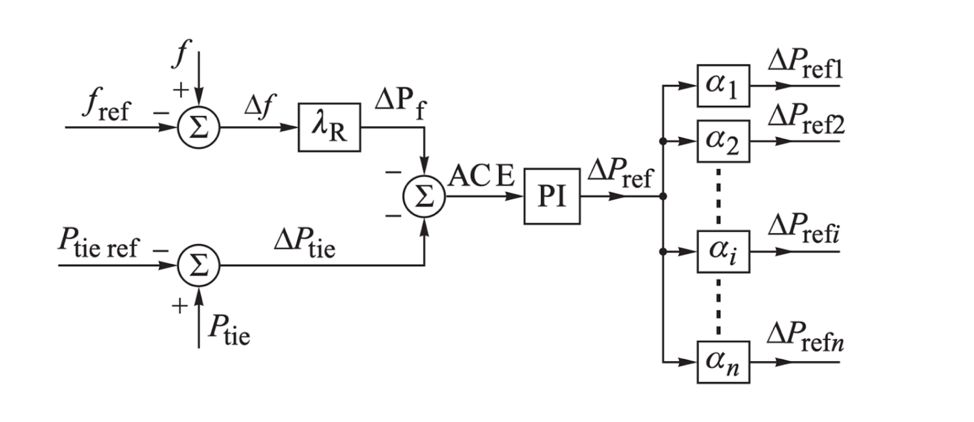
\includegraphics[width = \textwidth]{figure/3_1_Functional.png}
\caption{Functional diagram of a central regulator.}
\label{3_1_Functional}
\end{figure}

As seen in Figure \textcolor{red}{\ref{3_1_Functional}}, the frequency ($f$) will be measured in the local network and compared with the reference frequency to produce an amplified signal ($\Delta P_f$) that is proportional to the frequency deviation ($\Delta f$). For instance, if the frequency is smaller the reference frequency, then the signal $\Delta P_f$ will be negative. Thus, input signal ACE is positive according to the functional diagram. Therefore, output signal $\Delta P_f$ is positive and it will adjust the system by raising the reference value of the power. Then the system will have a new frequency value ($f_n_e_w$) that will go through the functional diagram again to compare the difference with the value of the reference frequency. ACE won’t be zero and the frequency won’t be stopped adding until we remove any error.\\

In this standard case, which ignores the existence of tie-line interchange error, the only condition to remove errors is the frequency deviation ($\Delta f$) equals to zero.\\

\begin{figure}[htbp]
\centering
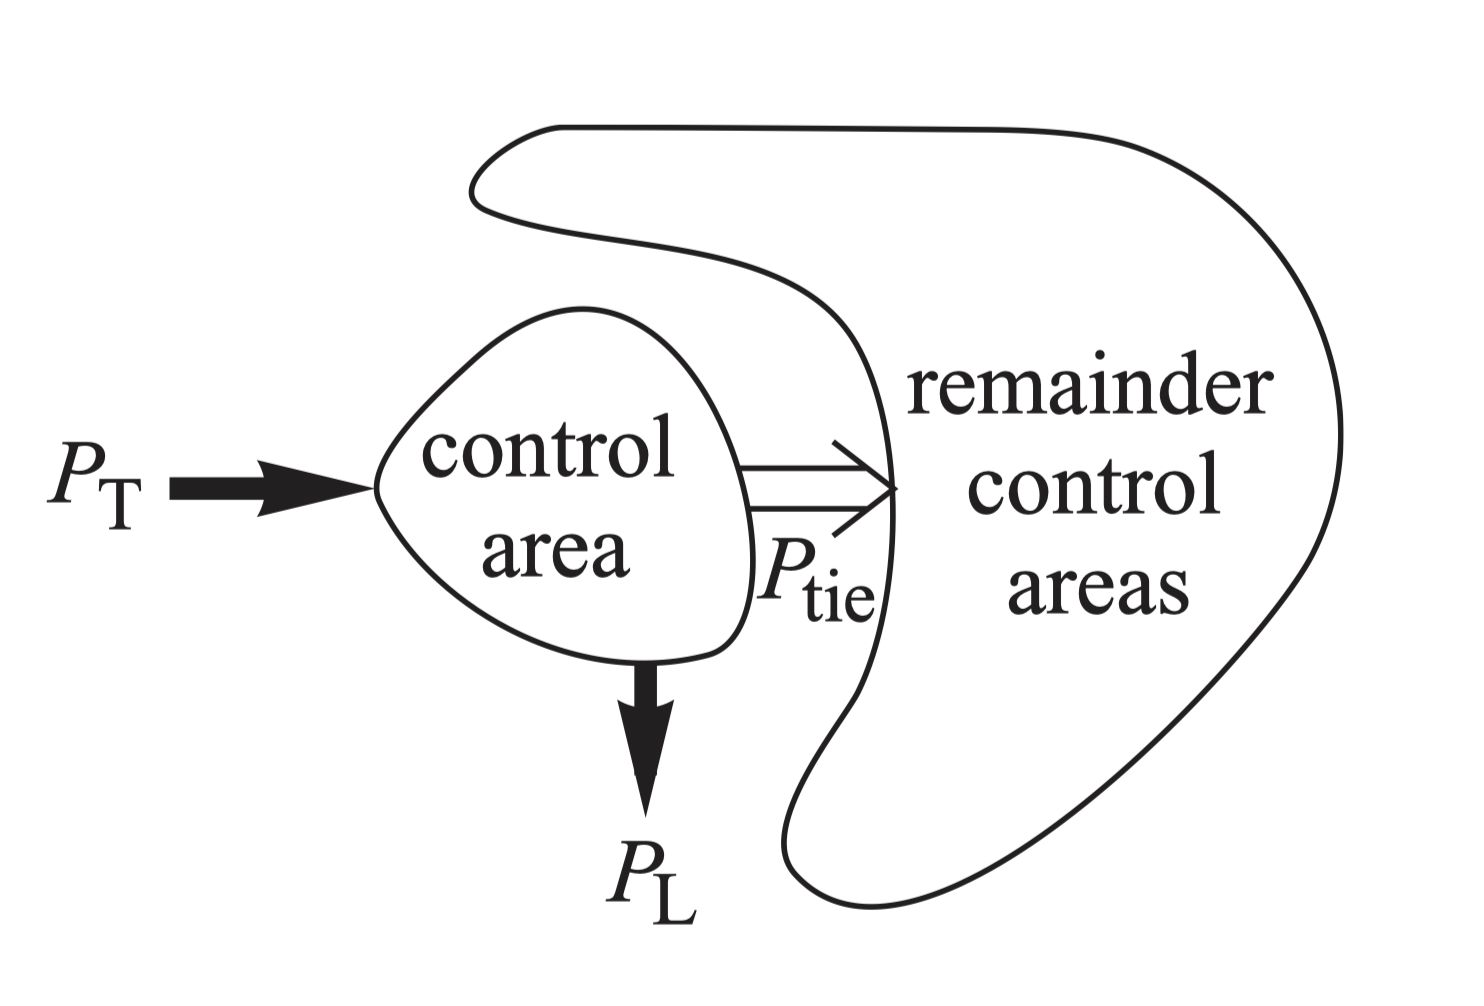
\includegraphics[width =\textwidth]{figure/3_1_Power.png}
\caption{Power balance of a control area.}
\label{3_1_Power}
\end{figure}

However, it would be more difficult if consider the situation of tie-line interchange error. In interconnected power systems, AGC is implemented in a way where each subsystem has its own regulator. As shown in Figure \textcolor{red}{\ref{3_1_Power}}, the power system is in equilibrium if the total power generation ($P_T$), the total power demand ($P_L$ ) and the net tie-line interchange power ( $P_t_i_e$ ) satisfy the condition in each subsystem:\\

\begin{equation} \label{eq1}
 P_T - (P_L + P_t_i_e) = 0
\end{equation}

The objective of each regulator of the subsystem is to maintain frequency at the nominal level and to maintain net tie-line interchanges from the given area at the scheduled values. If there is a disturbance in one subsystem, then regulators in each subsystem should try to restore the frequency and net tie-line interchanges. Each subsystem regulator should enforce an increased generation covering its own area power imbalance and maintain planned net tie-line interchanges.\\

As shown in Figure \textcolor{red}{\ref{3_1_Functional}}, to obtain a signal proportional to the tie-line interchange error ($\Delta P_t_i_e$), the information on power flows in the tie-lines is sent via telecommunication lines to the central regulator which compares it with the reference value. Then the signal ($\Delta P_f$) is added to the net tie-line interchange error ($\Delta P_t_i_e$) so that ACE is: \\
\begin{equation} \label{eq2}
 ACE = −\Delta P_f − \Delta P_t_i_e 
\end{equation}
The situation here is similar to the situation above, where we ignore tie-line interchange error, except for the condition to remove errors. In this book, it shows us zeroing of errors can be achieved in two ways: zeroing of both errors ($ P_t_i_e = 0 $ and $ f = 0 $) and achieving a compromise between the errors $(\Delta P_f + P_t_i_e = 0 $ & or $ P_f = - \Delta P_t_i_e $).\\



\section{PID Controller} %3.2
PID controller can be written in the following equation:

\begin{equation} \label{eq3}
 u(t) = k_p e(t) + k_i \int_{0}^{t} e(\tau) d\tau + k_d \frac{d e}{d t}
\end{equation}

 where u is the control signal and e is the error. The nominal value is also called the reference value or the setpoint. The controller’s output is therefore summed by three terms: the P-term, the I-term, and the D-term. The P-term is proportional to the error and its amplification factor is $k_p$. The I-term is proportional to the integral of the error and its amplification factor is $k_i$. The D-term is proportional to the derivative of the error and its amplification factor is $k_d$.\\
 
 The function of the P-term is trying to send a control signal proportional to the error. For example, there is a signal whose value is 90 and we hope it can approach to 100 using P-term only. The error now is (100 - 90 = 10). Assumed that $k_p$ equals to 0.5, then control signal becomes (10 x 0.5 = 5). The new signal becomes (90 + 5 = 95). If we continue to repeat this flow, we will find the new signal turns to 97.5, 98.75 and 99.375. It seems like the new signal is approaching to our nominal value and it will approach to the nominal value if we continue updating the signal.\\
 

However, there are two situations that we cannot ignore. Firstly, steady-state error occurs if $k_p$ is not set well. For example, if $k_p$ equals to 2, the error will be 20 and the new signal will be 110, 90, 110, 90,… The signal can not be restored to the nominal one forever. \\

The second situation is that, in reality, the signal is not perfect and it has its own errors. In the first example above, we choose 0.5 as our amplification factor ($k_p$) and thus the first new signal will be 95. However, it is a possible and common situation that the new signal will be lost its signal value by 5 every time every time after the control. Finally, the signal will remain 90 and the error will be 10 forever. \\

\begin{figure}[htbp]
\centering
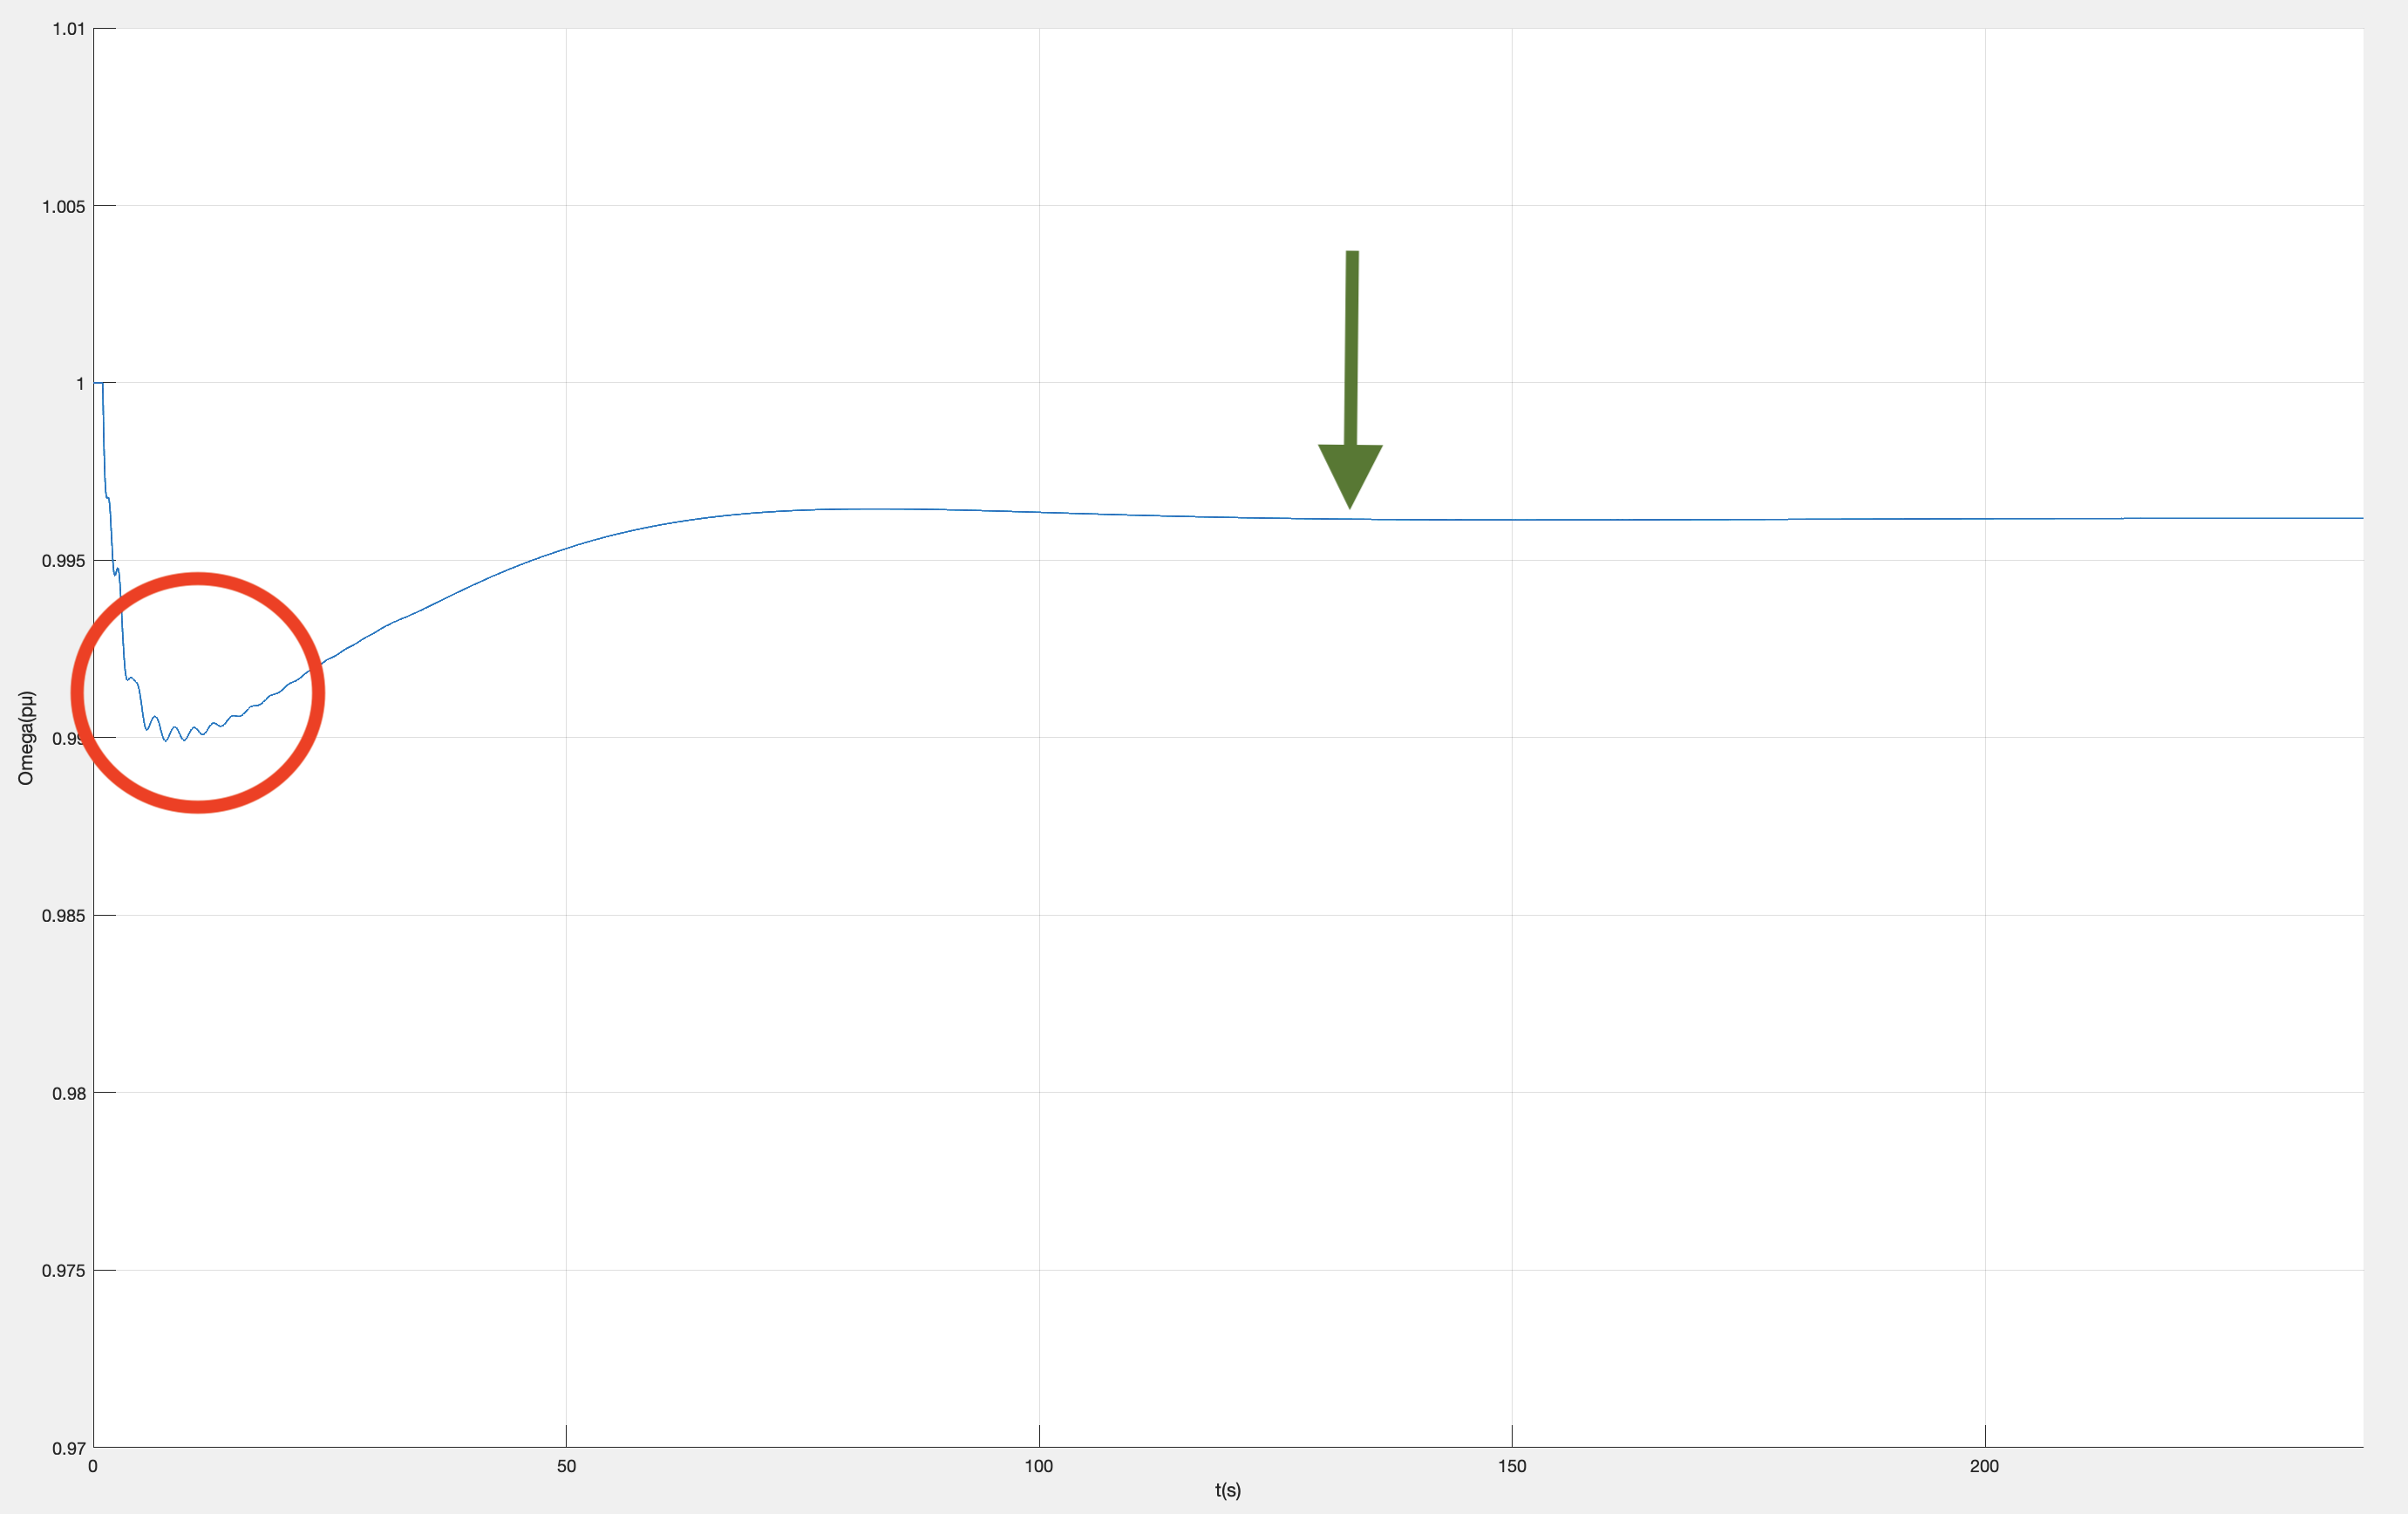
\includegraphics[width = \textwidth]{figure/3_2_steady.png}
\caption{Steady-state error and high frequency component in a signal.}
\label{3_2_steady}
\end{figure}

In reality, whatever the automobile control system, the electronic compass control system or the Automatic Generation Control, the steady-state errors occurs if we use P control only.\\

We introduce the I-term to remove such a steady-state error. Briefly, the integral of the error will accumulate the previous errors and the I-term is proportional to the integral of the error, which means the I-term is proportional to previous accumulated errors. The integral of the error will not be zero, unless the error is removed. Controlling signal will be larger and the new signal value will approach to the nominal value gradually.\\

To the D-term, it is proportional to the derivative of the error. In another way, the D-term is proportional to the gradient of the signal. Thus, the D-term will amplify the high frequency component in the signal and will disturb the system.\\


\section{PI Control Model} %3.3
At this point, we are equipped with all the building blocks. Let’s first recap a PI control model. In PI control, we need to know the value of error and the value of integral of the error. Error is defined by the difference between the nominal value and the signal. In AGC, the nominal value is nominal frequency and the signal is the actual frequency sending into the controller.\\

To the integral of the error,  it is should be realised that using discrete mathematics is helpful. In discrete mathematics, the value of integral of the error is the accumulated error. Thus, in programming, we can use time-step to help calculating the integral of the error.  Detailedly, in program, we can represent output as\\

\begin{figure}[htbp]
\centering
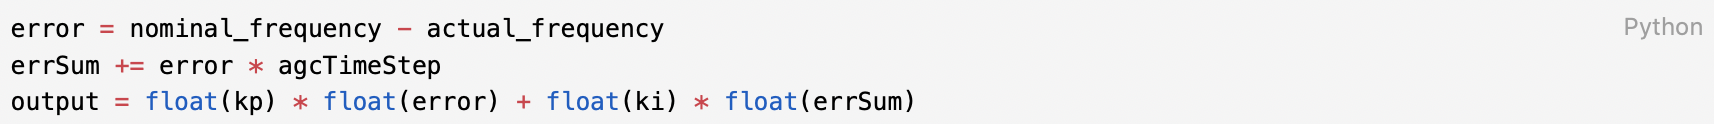
\includegraphics[width = \textwidth]{figure/3_3_code1.png}
%\caption{ }
\label{3_3_code1}
\end{figure}

where nominal frequency is 1.0 and we can directly get actual frequency from the simulation.\\

Next, we should send output signal to generators through the command,\\

\begin{figure}[htbp]
\centering

\includegraphics[width = \textwidth]{figure/3_3_code2.png}
%\caption{ }
\label{3_3_code2}
\end{figure}

where, 'gensName' is the name of generator such as g1, g2 or g9. '1/gensWeight' is $\alpha$ in the Figure \textcolor{red}{\ref{3_1_Functional}}. We use $\alpha$ to ask power proportional to these generators' nominal power. \\

Furthermore, we need to consider dead band. For instance, it is considered as approaching the set point if the error is 0.000009. Thus,\\

\begin{figure}[htbp]
\centering
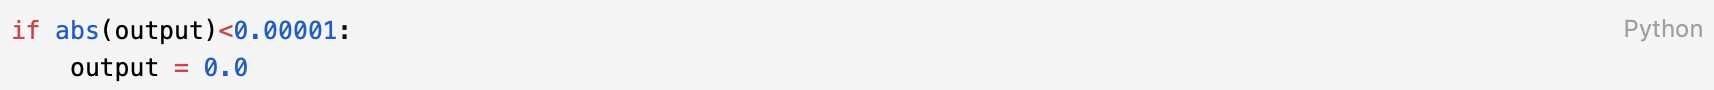
\includegraphics[width = \textwidth]{figure/3_3_code3.png}
%\caption{ }
\label{3_3_code3}
\end{figure}

We get the input from the existing smart grid simulator and send output to the existing smart grid simulator via our controller. Thus, a communication layer is formed.\\

Multiple hardcoded parameters, like the disconnected generator, the generators we asked for their power, amplification factor and time delay, are removed and added into main function so we can test our system comprehensively and easily.\\


\section{Tuning Methodology } %3.4
\subsection{Tuning Model} %3.4.1
Imagine if we have a 2d plane with the horizontal axis kp and the vertical axis ki, we can use the points on the plane to represent all the acceptable combination of kp and ki.\\

\begin{figure}[!htbp]
\minipage{0.33\textwidth}
  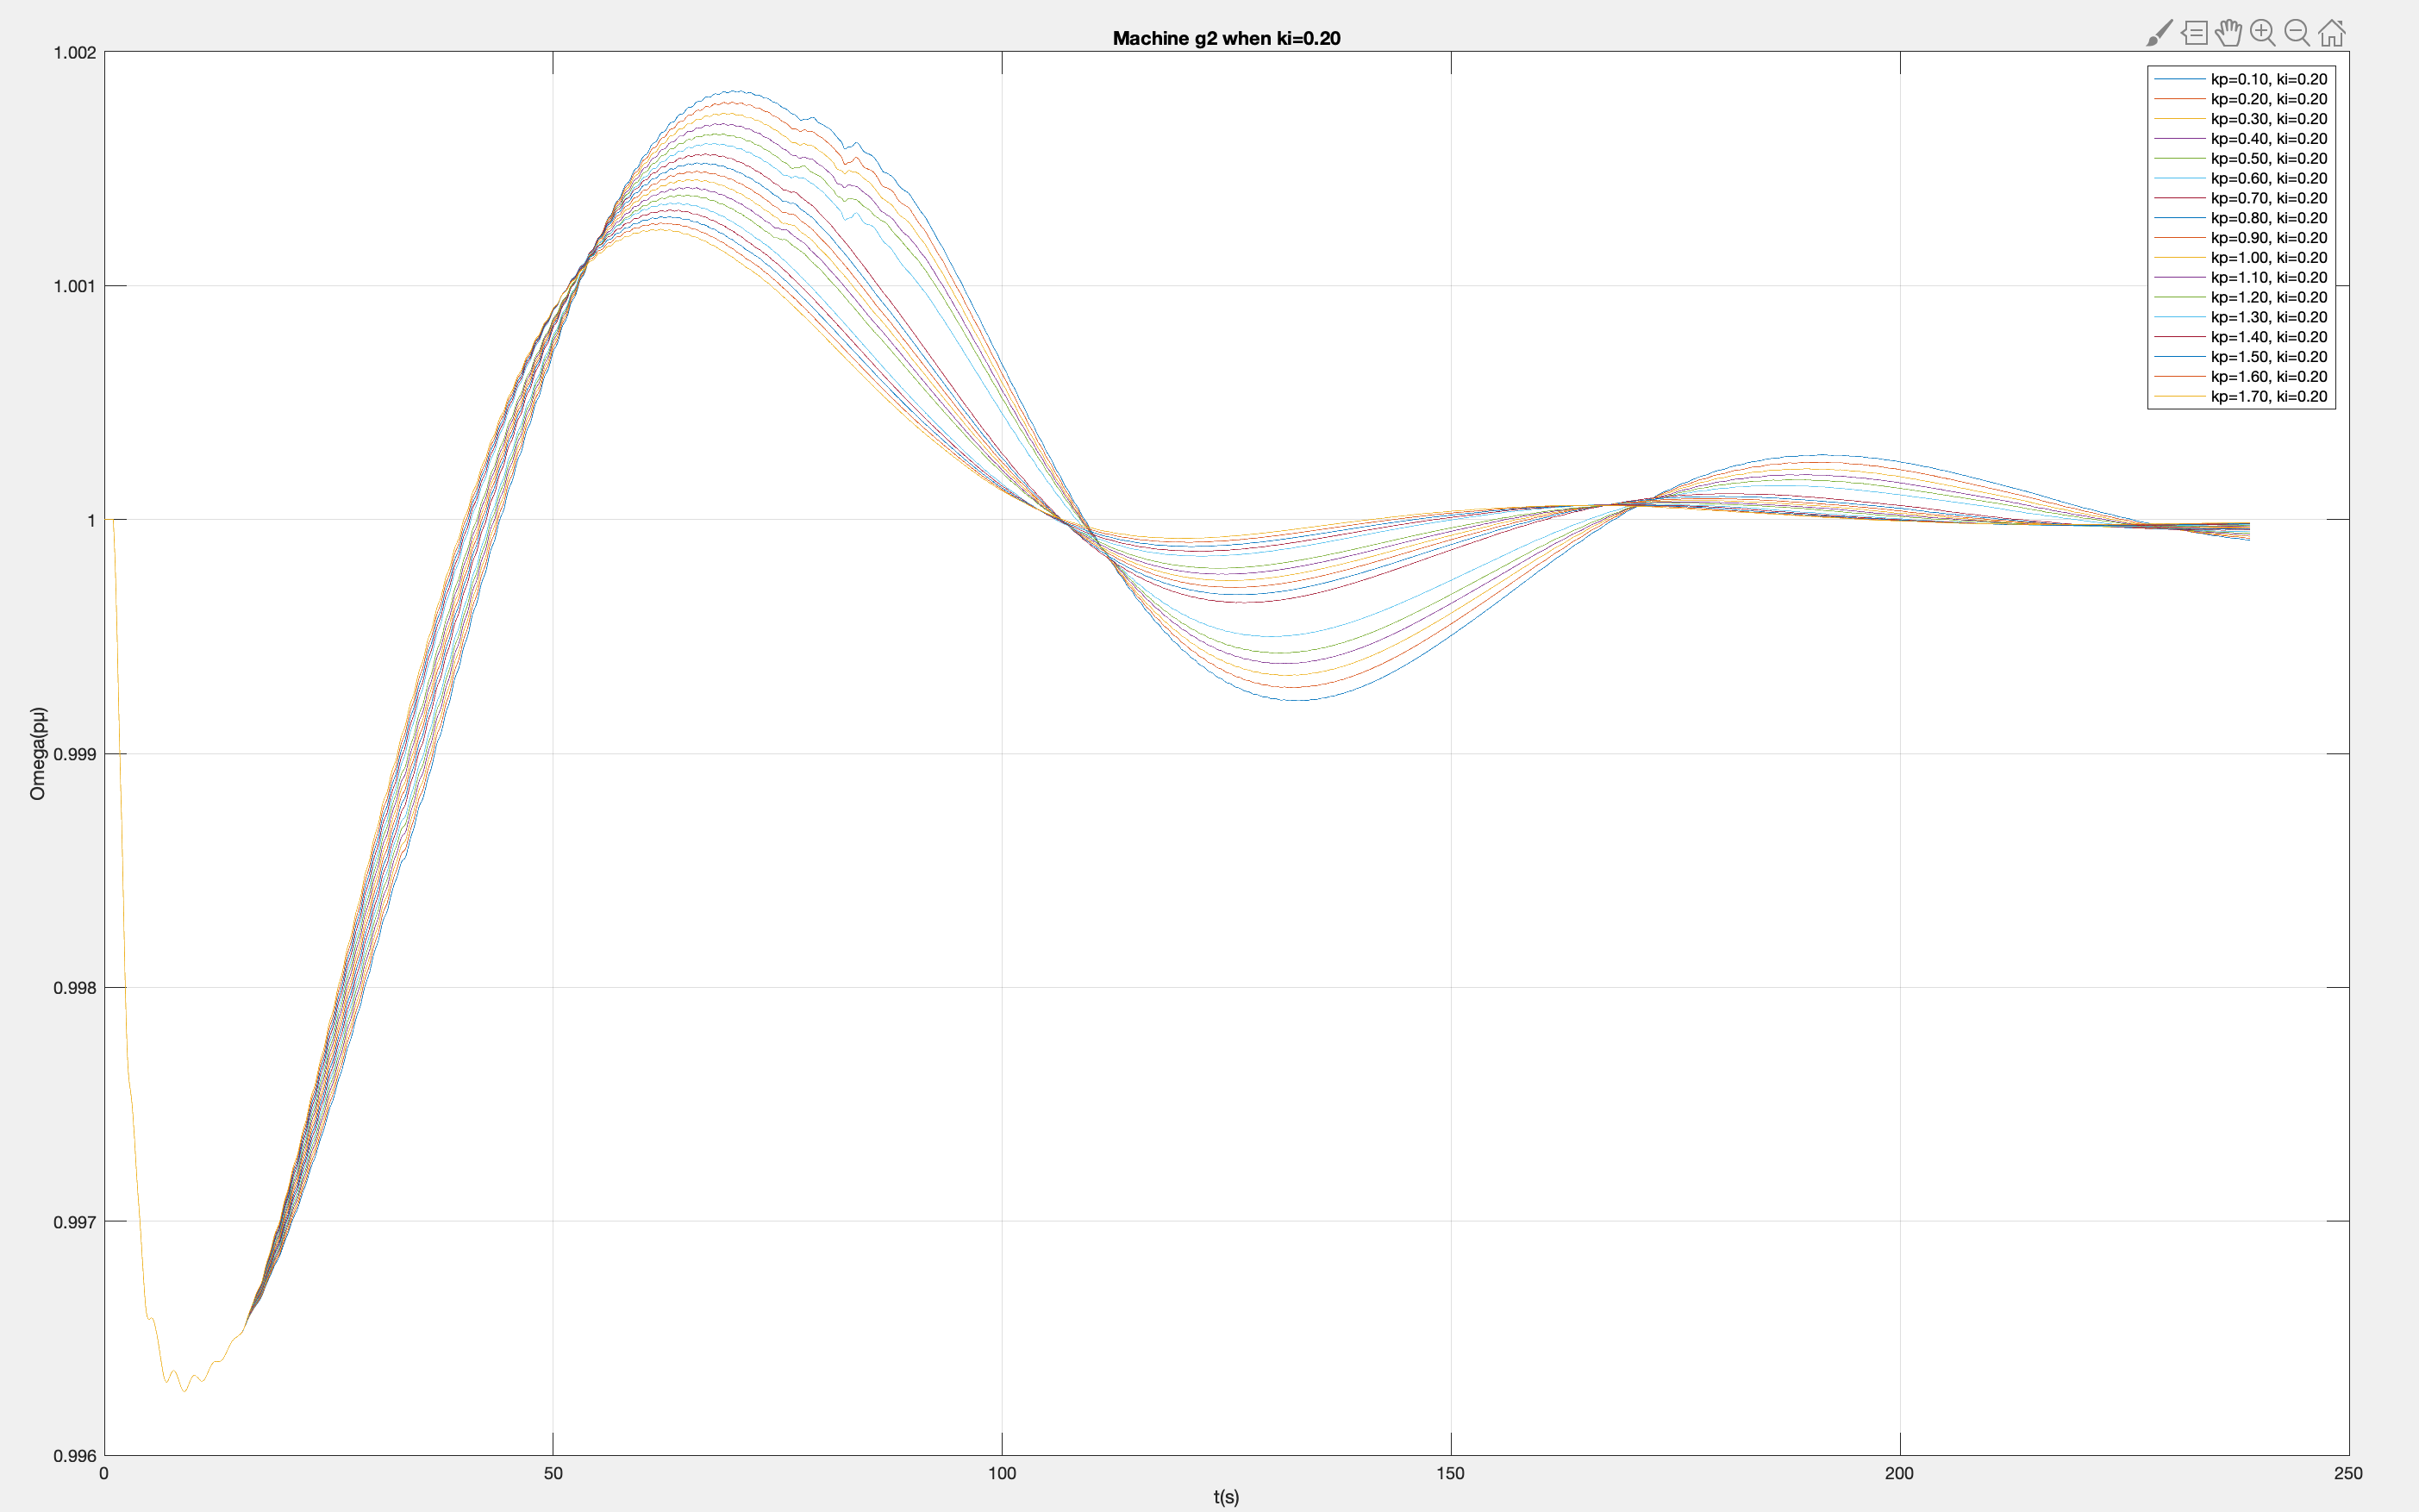
\includegraphics[width= \linewidth]{figure/3_4_1_tune_ki_1.png}
  %\caption{A really Awesome Image}\label{fig:awesome_image1}
\endminipage\hfill
\minipage{0.33\textwidth}
  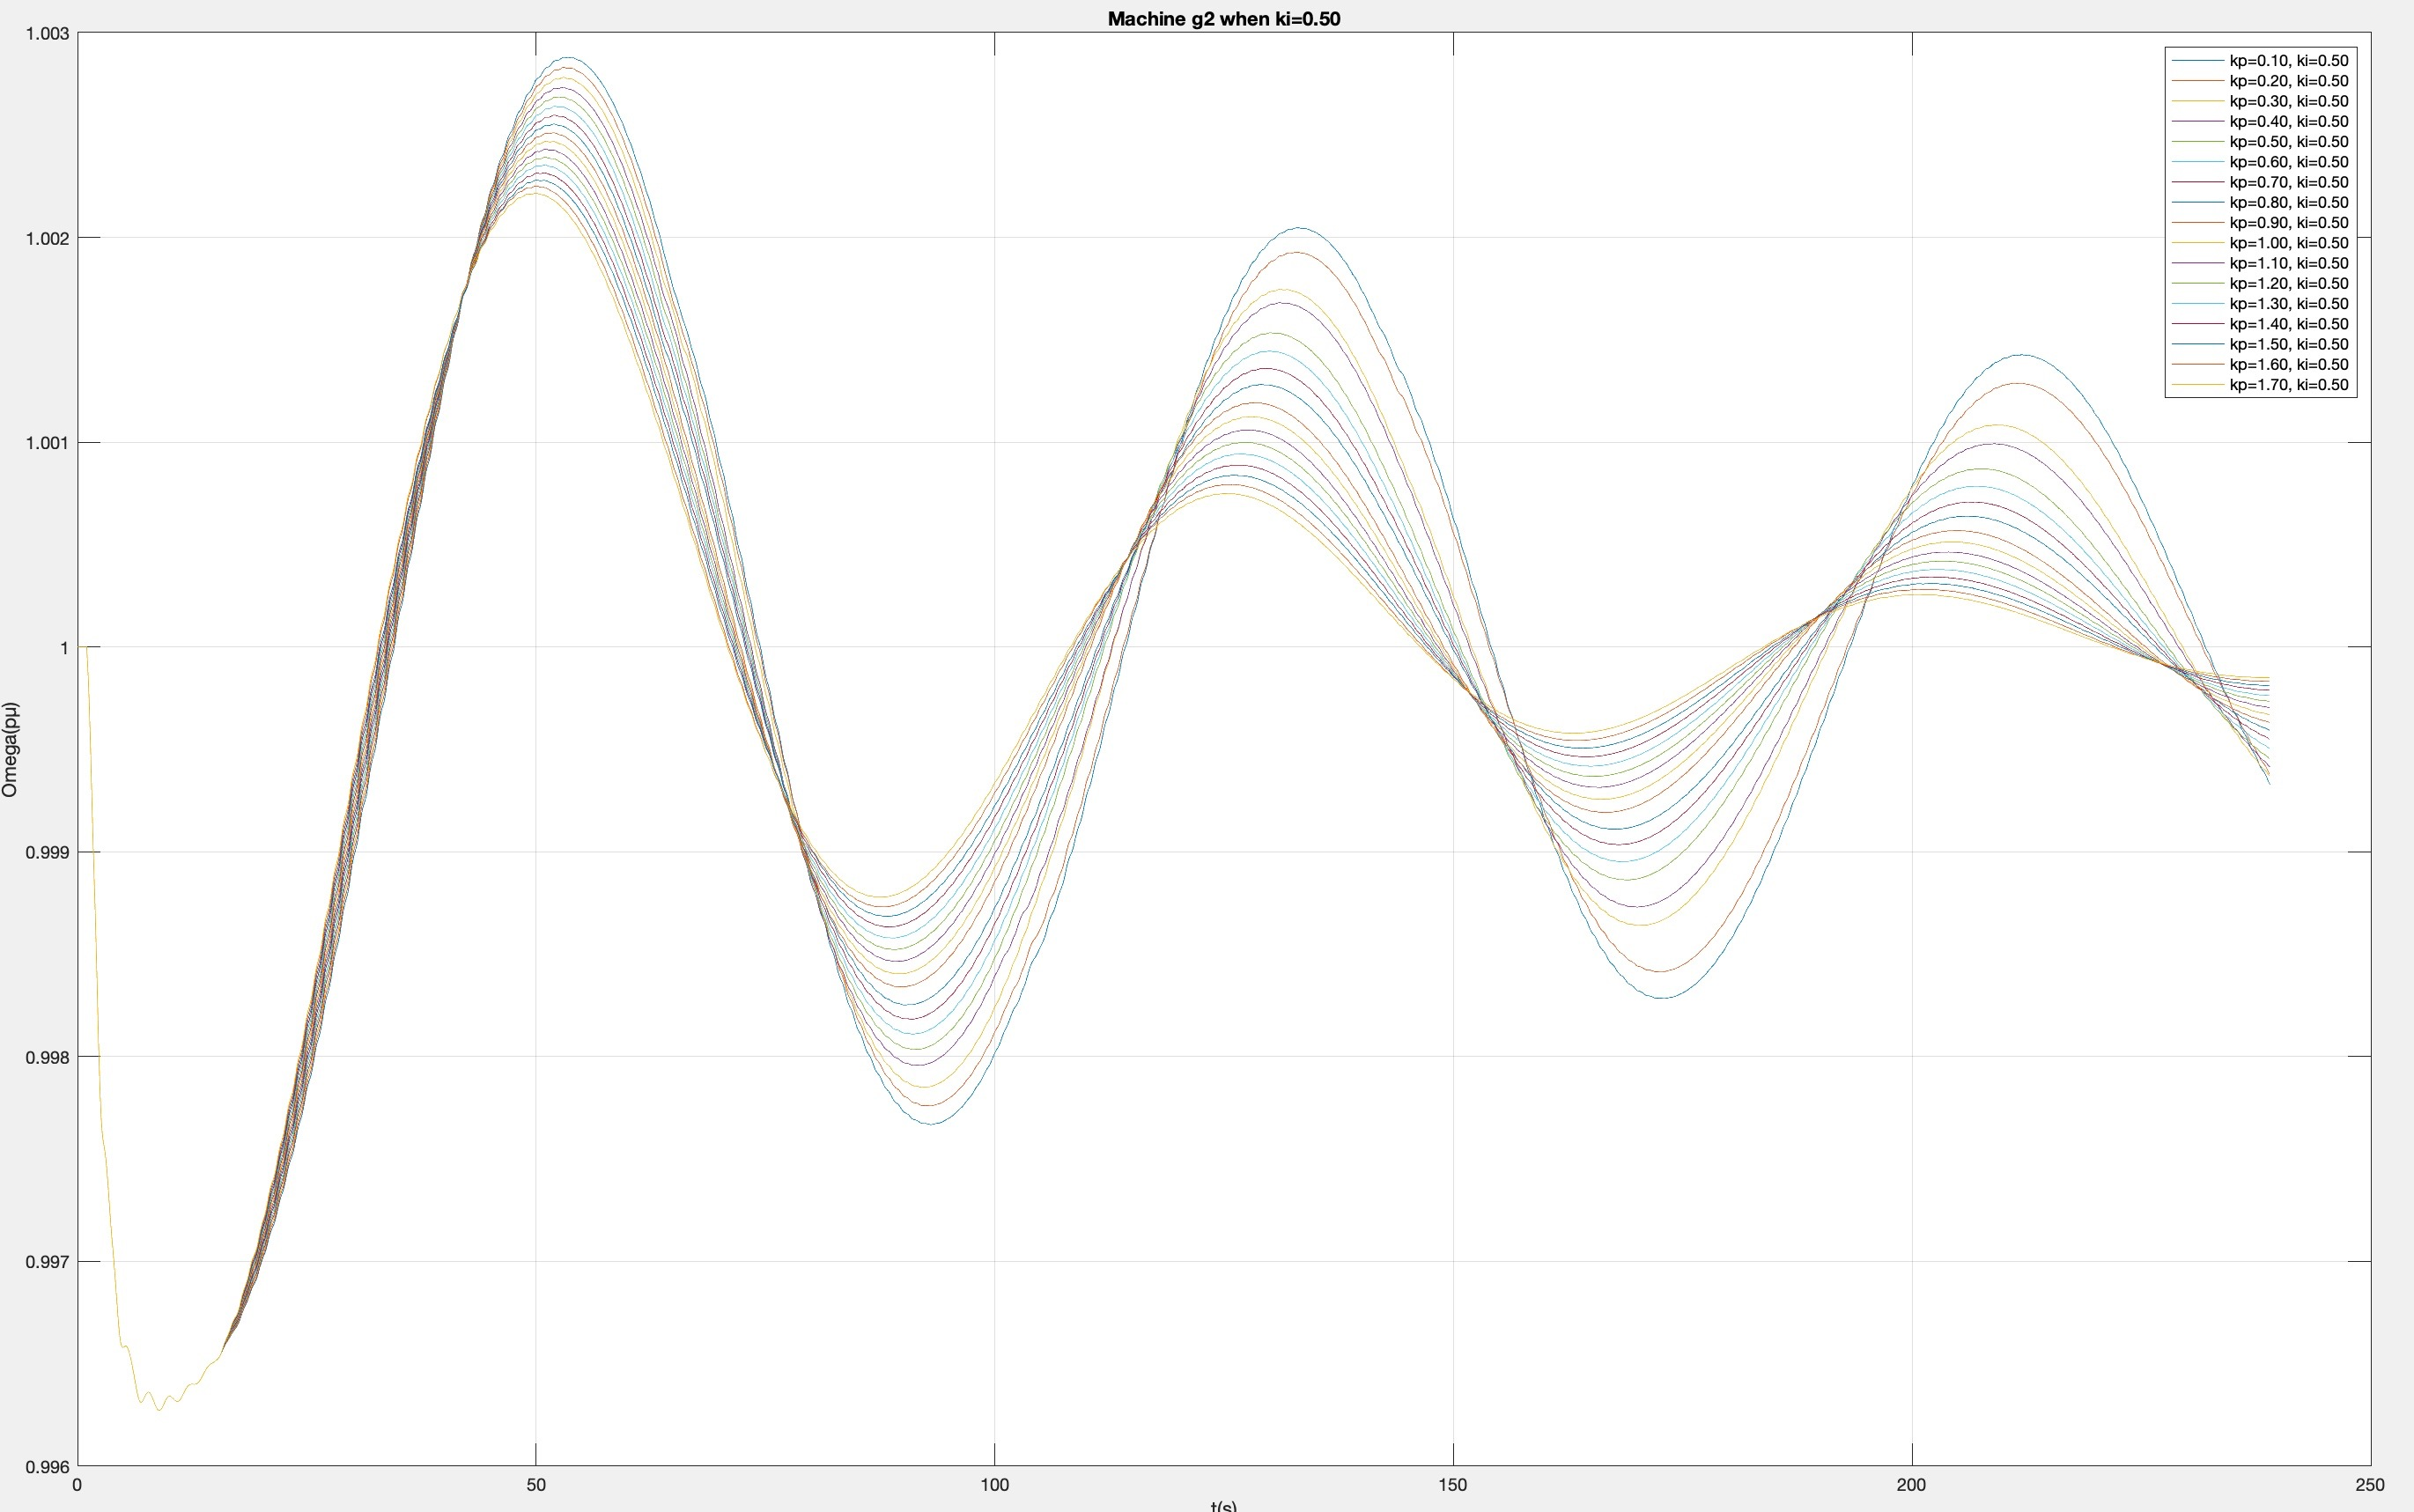
\includegraphics[width= \linewidth]{figure/3_4_1_tune_ki_2.jpeg}
  %\caption{A really Awesome Image}\label{fig:awesome_image2}
\endminipage\hfill
\minipage{0.33\textwidth}%
  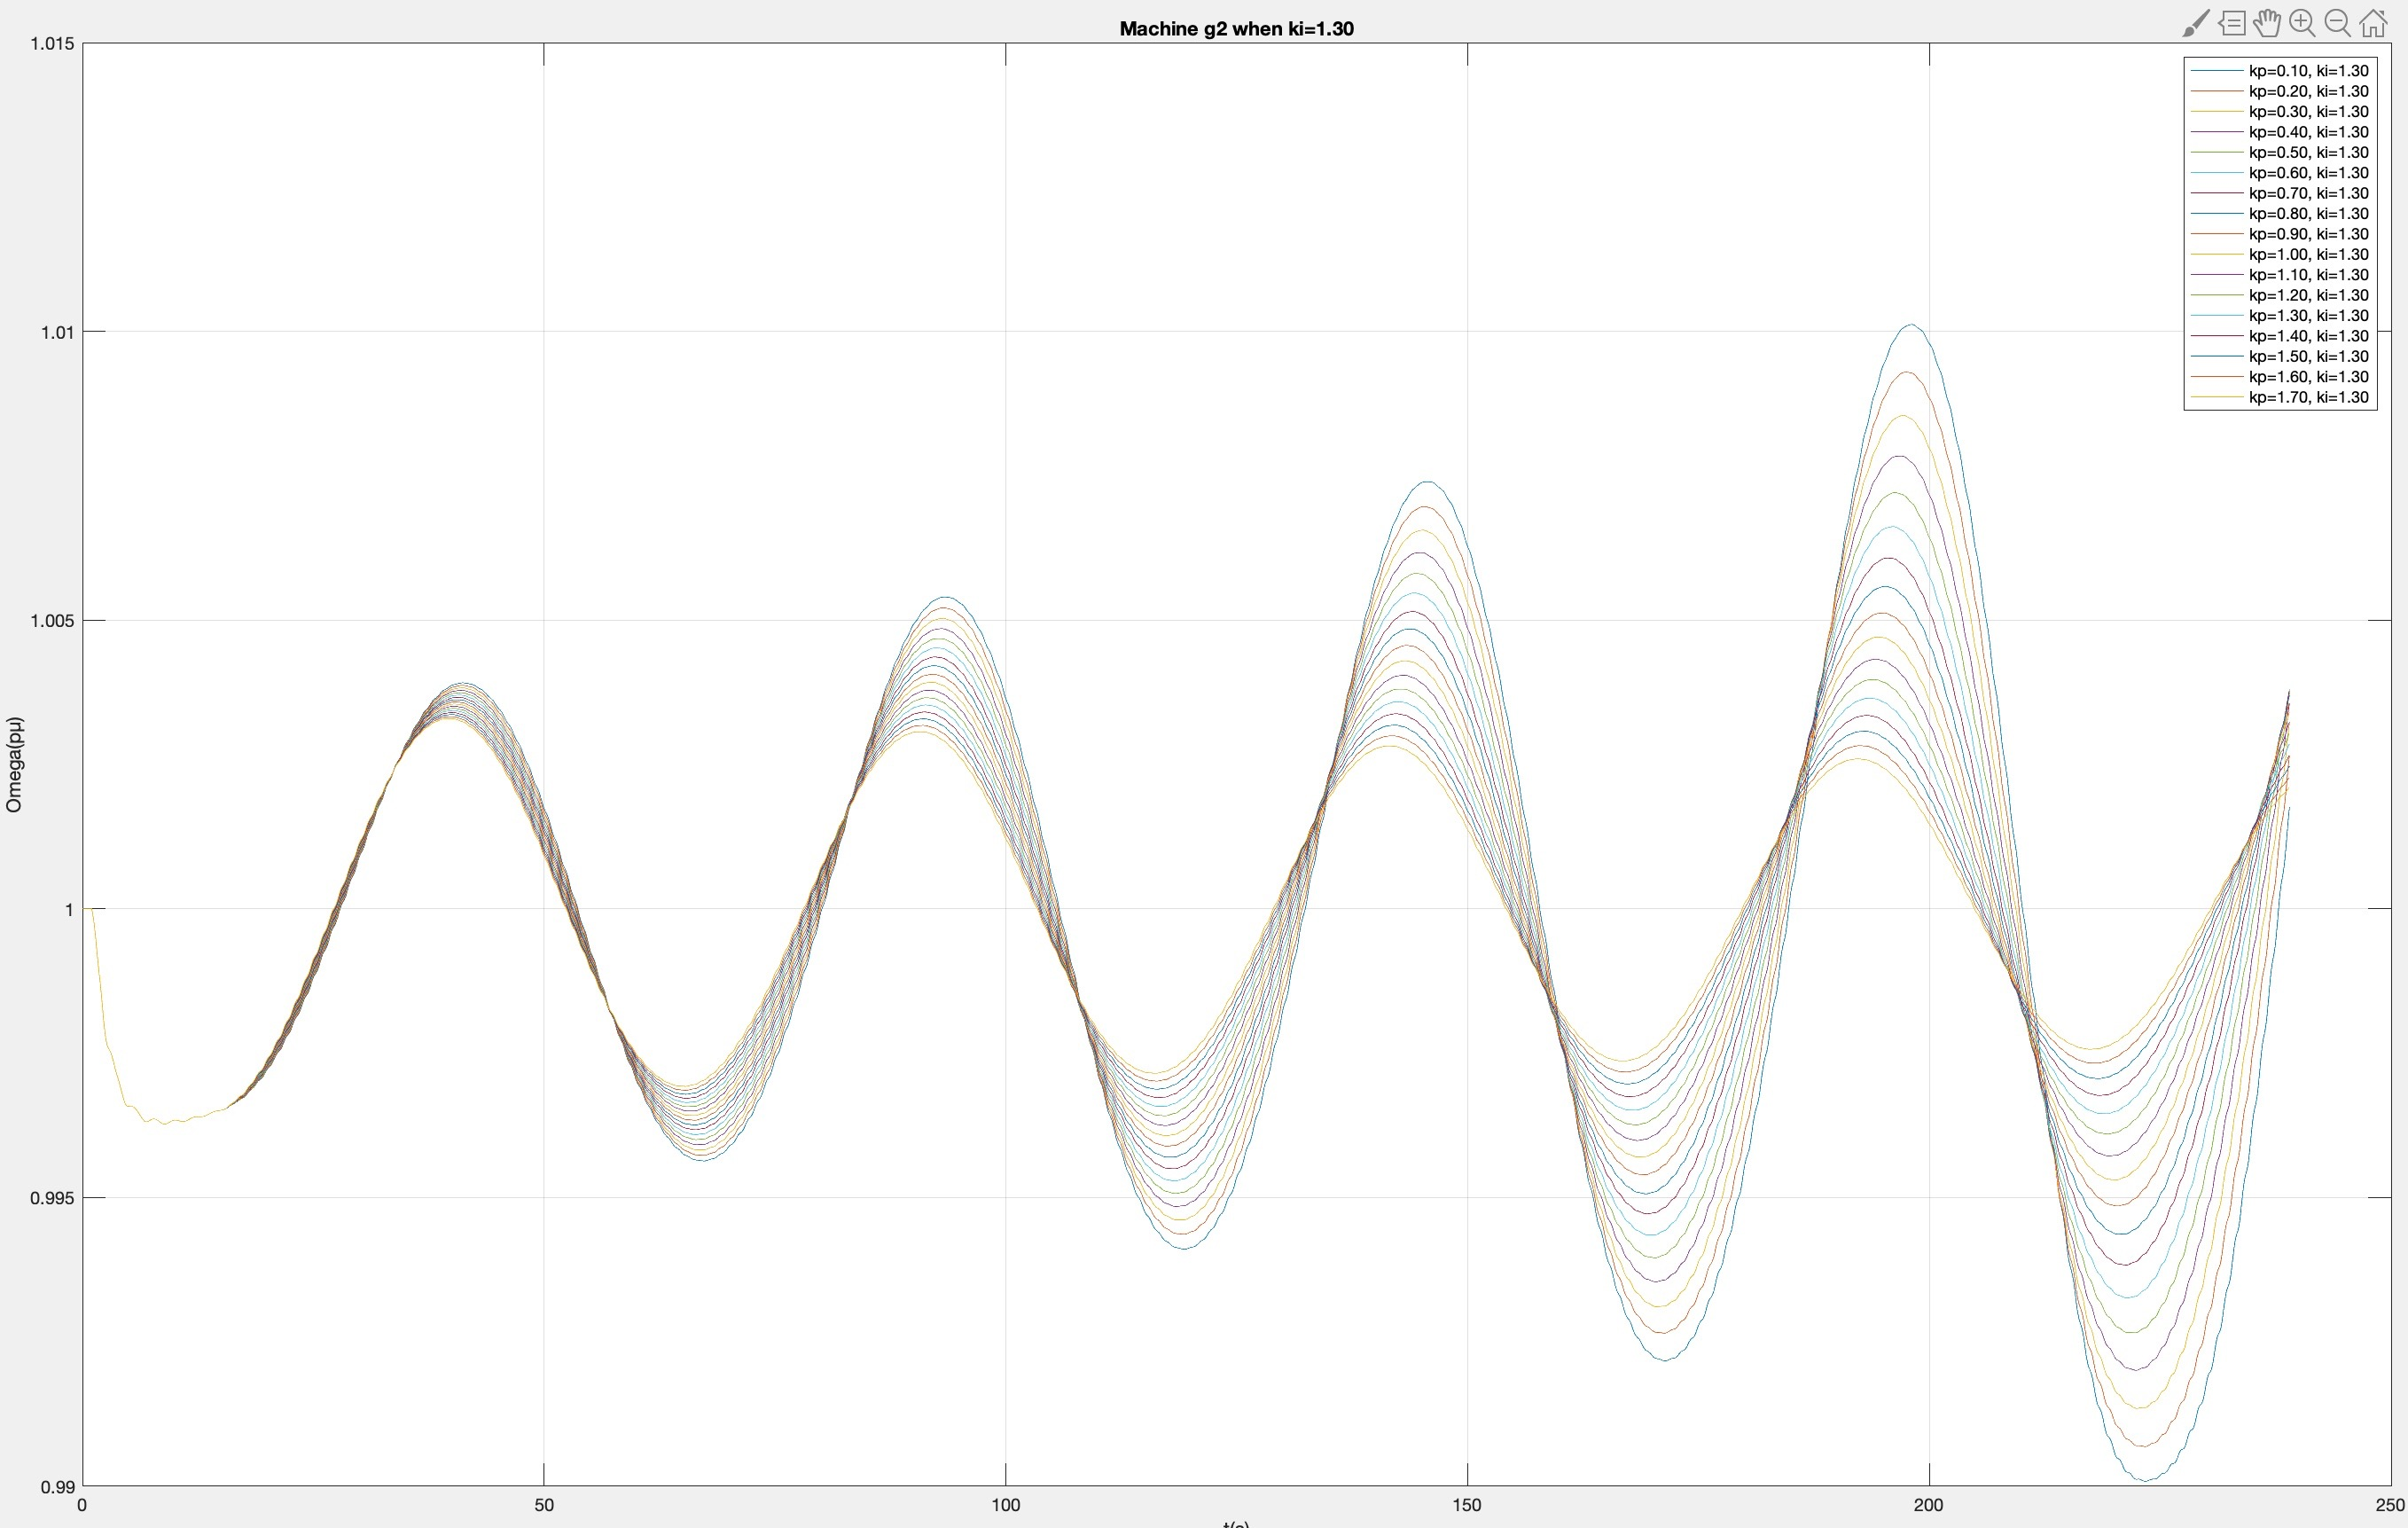
\includegraphics[width= \linewidth]{figure/3_4_1_tune_ki_3.jpeg}
  %\caption{A really Awesome Image}\label{fig:awesome_image3}
\endminipage
\caption{PI Control: ki = 0.2; ki = 0.5; ki = 1.3}
\label{3_4_1_larger_ki}
\end{figure}


The reason for this is that neither kp nor ki can be infinitely magnified. Kp is the amplifier factor of D-term and it represents how quickly the error can be corrected. The if kp is larger, the overshoot of the corrected signal will be larger. The kp will have a limit because there is an acceptable range for the signal in the test case scenario. For instance, in Nordic test case scenario, the limit is ±0.2\%. In other words, the range of signal is from 0.998 $p\mu$ to 1.002$p\mu$.\\

Ki is the amplifier factor of the I-term. The signal will have too many oscillations and it will not be settled if we keep increasing the value of ki. 
However, the signal needs to be settled before a specific time in reality and it makes sure the signal will be no chance of excessive oscillation. Thus, ki is limited.\\

One of the objectives of this project is to find the best combination of amplifier factors, i.e. kp and ki. To obtain it, we need to find the limit of kp and ki.\\

The idea of bisection method is used to find the limit of kp and ki.\\

Firstly, a large kp will be chosen as a tuning value and we will test whether the new signal is acceptable whatever the value of ki is. To simplify the model, we choose ki being from 0.1 to the value of kp and the step of ki is dependent to the value of kp. For instance, the range of ki will be between 0.1 and 500.1 if kp is 500.1. From the knowledge we discussed before, the signal has small probability not having a large overshoot. Thus, the range of ki can be given a large step, like 100.0. We do not need to worry about such a large step will filter some acceptable results. The purpose of this step is not to find all the acceptable results. The purpose of tuning kp and ki is not finding all the possible values. We hope to find a general relationship between kp and ki and it is helpful to find the impact of time delay afterwards.\\

Secondly, we check if the signal is acceptable by importing data into an analytical model written by MATLAB. The purpose of this step is to check whether ki is existing. \\

If ki exists (i.e. there is one acceptable result at least), for instance, ki equals to 200.1, we need to make sure there will be no solutions when increasing ki by its step. Then, we can judge that the limit of the kp is between 200.1 and  200.1 + the step of kp). Thus, we have a range of kp which is between 0.1 and (200.1 + the step of kp). If the step of kp is 10, the range of kp will be from 0.1 to 210.1. Normally, we can directly tune kp and ki between 0.1 and 210.1. If we set the step of kp and ki to 10, there will be just 484 results and it is positive to the time management. However, in many cases, the maximum value of ki will be smaller than the step of ki! That means you will see ki equalling to 0.1 for all the kp cases. The data is meaningless to us. Thus, it is a good way to tune the step of ki according to the relative maximum value of ki.\\

If ki exists in another way, for instance, kp equals to 200.1 and ki equals to 5.1 when the step of ki is 5.0. The result is acceptable but we need to increase the value of kp to make sure ki will not exist when kp equals to (kp + the step of kp).\\

If ki does not exist, for instance, kp equalling to 500.1 is unacceptable, according to bisection method, we can test the simulations and tune kp between 0.1 and 250.1. We repeat the method above until we find the limit of kp and ki.\\


\subsection{Analytical Models} %3.4.2
The first analytical model will generate two different kinds of excel files. One of them is named as ori.xlsx. This is a file saving all the acceptable points. For another kind of files, their names are related to the value of time delay. For instance, if time delay is 0.01 seconds, the file name will be td\_0.01s\_xlsx. It will store all the acceptable points when delay is 0.01 seconds.\\

Importantly, we define 'SettlingTimeThreshold' , a MATLAB variant, to 0.02, so time it takes for the error between the response and the steady-state response to fall to within 2\% of nominal value.\\

\begin{figure}[htbp]
\centering
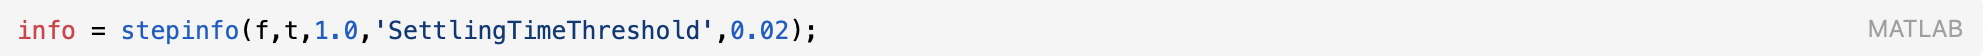
\includegraphics[width = \textwidth]{figure/3_4_2_code4.png}
%\caption{ }
\label{3_4_2_code4}
\end{figure}

In the first analytical model , we check if simulation results are acceptable via our MATLAB program if we have collected data. Firstly, we import data from simulations. Then, we will limit both the overshoot and settling time as required via a MATLAB module: stepinfo. The data will be filtered if overshoot or the settling time is not in the range we set.\\

\begin{figure}[htbp]
\centering
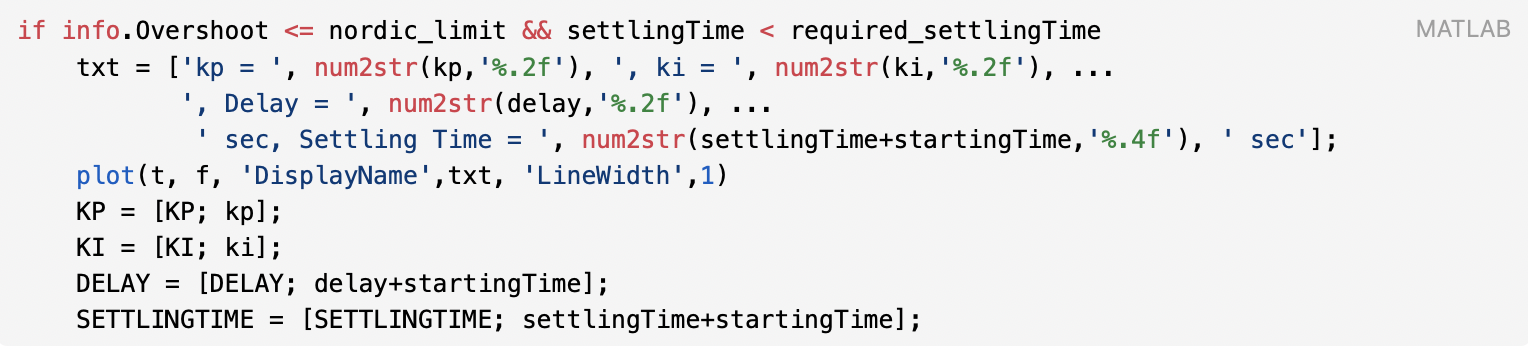
\includegraphics[width = \textwidth]{figure/3_4_2_code5.png}
%\caption{ }
\label{3_4_2_code5}
\end{figure}


As you can see, if the signal is acceptable, its parameters, i.e. kp, ki and time delay, will be save in prepared lists. The lists will be transferred into the two kinds of excel files.\\

The second analytical model helps finding which combination of kp and ki will have a minimum settling time with a fixed delay. The thought is as following. Firstly, we will import an excel file, whose name is related to the value of delay,  that is generated by the last step. Then, we will find the minimum of the settling time via function min() in Python. Finally, we will find kp, ki and delay value related to this minimum settling time value and export them into another excel file named as best\_points.xlsx.\\

The third analytical model helps finding the best combination of kp and ki. Firstly, we import data from ori.csv that can be transferred directly by ori.xlsx file. Then, we will calculate the average settling time for each combination of kp and ki. However, it is invalid that a combination is not acceptable for all the time delay. Thus, we need to add a limitation factor to make sure the best combination is valid. For instance, if there are 21 different time delay, we can use:\\

\begin{figure}[htbp]
\centering
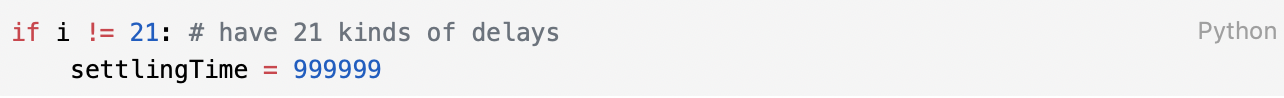
\includegraphics[width = \textwidth]{figure/3_4_2_code6.png}
%\caption{ }
\label{3_4_2_code6}
\end{figure}

to filter some unacceptable results. Finally, we have all the average settling time. We will find the minimum average settling time via the exported csv file named rank\_average\_settling\_time.csv.\\

The fourth analytical model helps sorting out the combination’s selling time with different time delay from ori.csv file. It will be as one of the inputs of our fifth analytical model.\\

The fifth analytical model helps plotting a 3D triangle surface plot. In all, it draws a 3d plot from the data in ori.xlsx. After defining x axis, y axis and z axis, we use:\\

\begin{figure}[htbp]
\centering
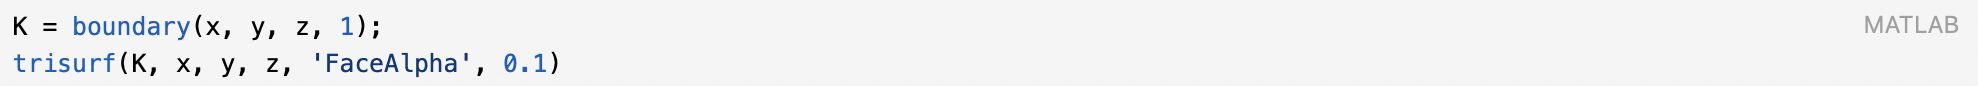
\includegraphics[width = .999\textwidth]{figure/3_4_2_code7.png}
%\caption{ }
\label{3_4_2_code7}
\end{figure}

to draw a triangle surface plot. Besides, it highlights the results from the second analytical model and the fourth analytical model. With a 3D triangle surface plot, we can clearly understand the impacts of the time delay.\\


\part{Test Case Scenario (Nordic) }
\chapter{Low Time Delay}
\label{Chapter4} %4
\section{Hypothesis} %4.1
\subsection{Hardware Hypothesis} %4.1.1

In this Chapter, we use the algorithms described in the Chapter 3 to test the well-known Nordic system. One-line diagram of the Nordic test system is  shown in Figure \textcolor{red}{\ref{4_1_1_nordic}}.\\

\begin{figure}[htbp]
\centering
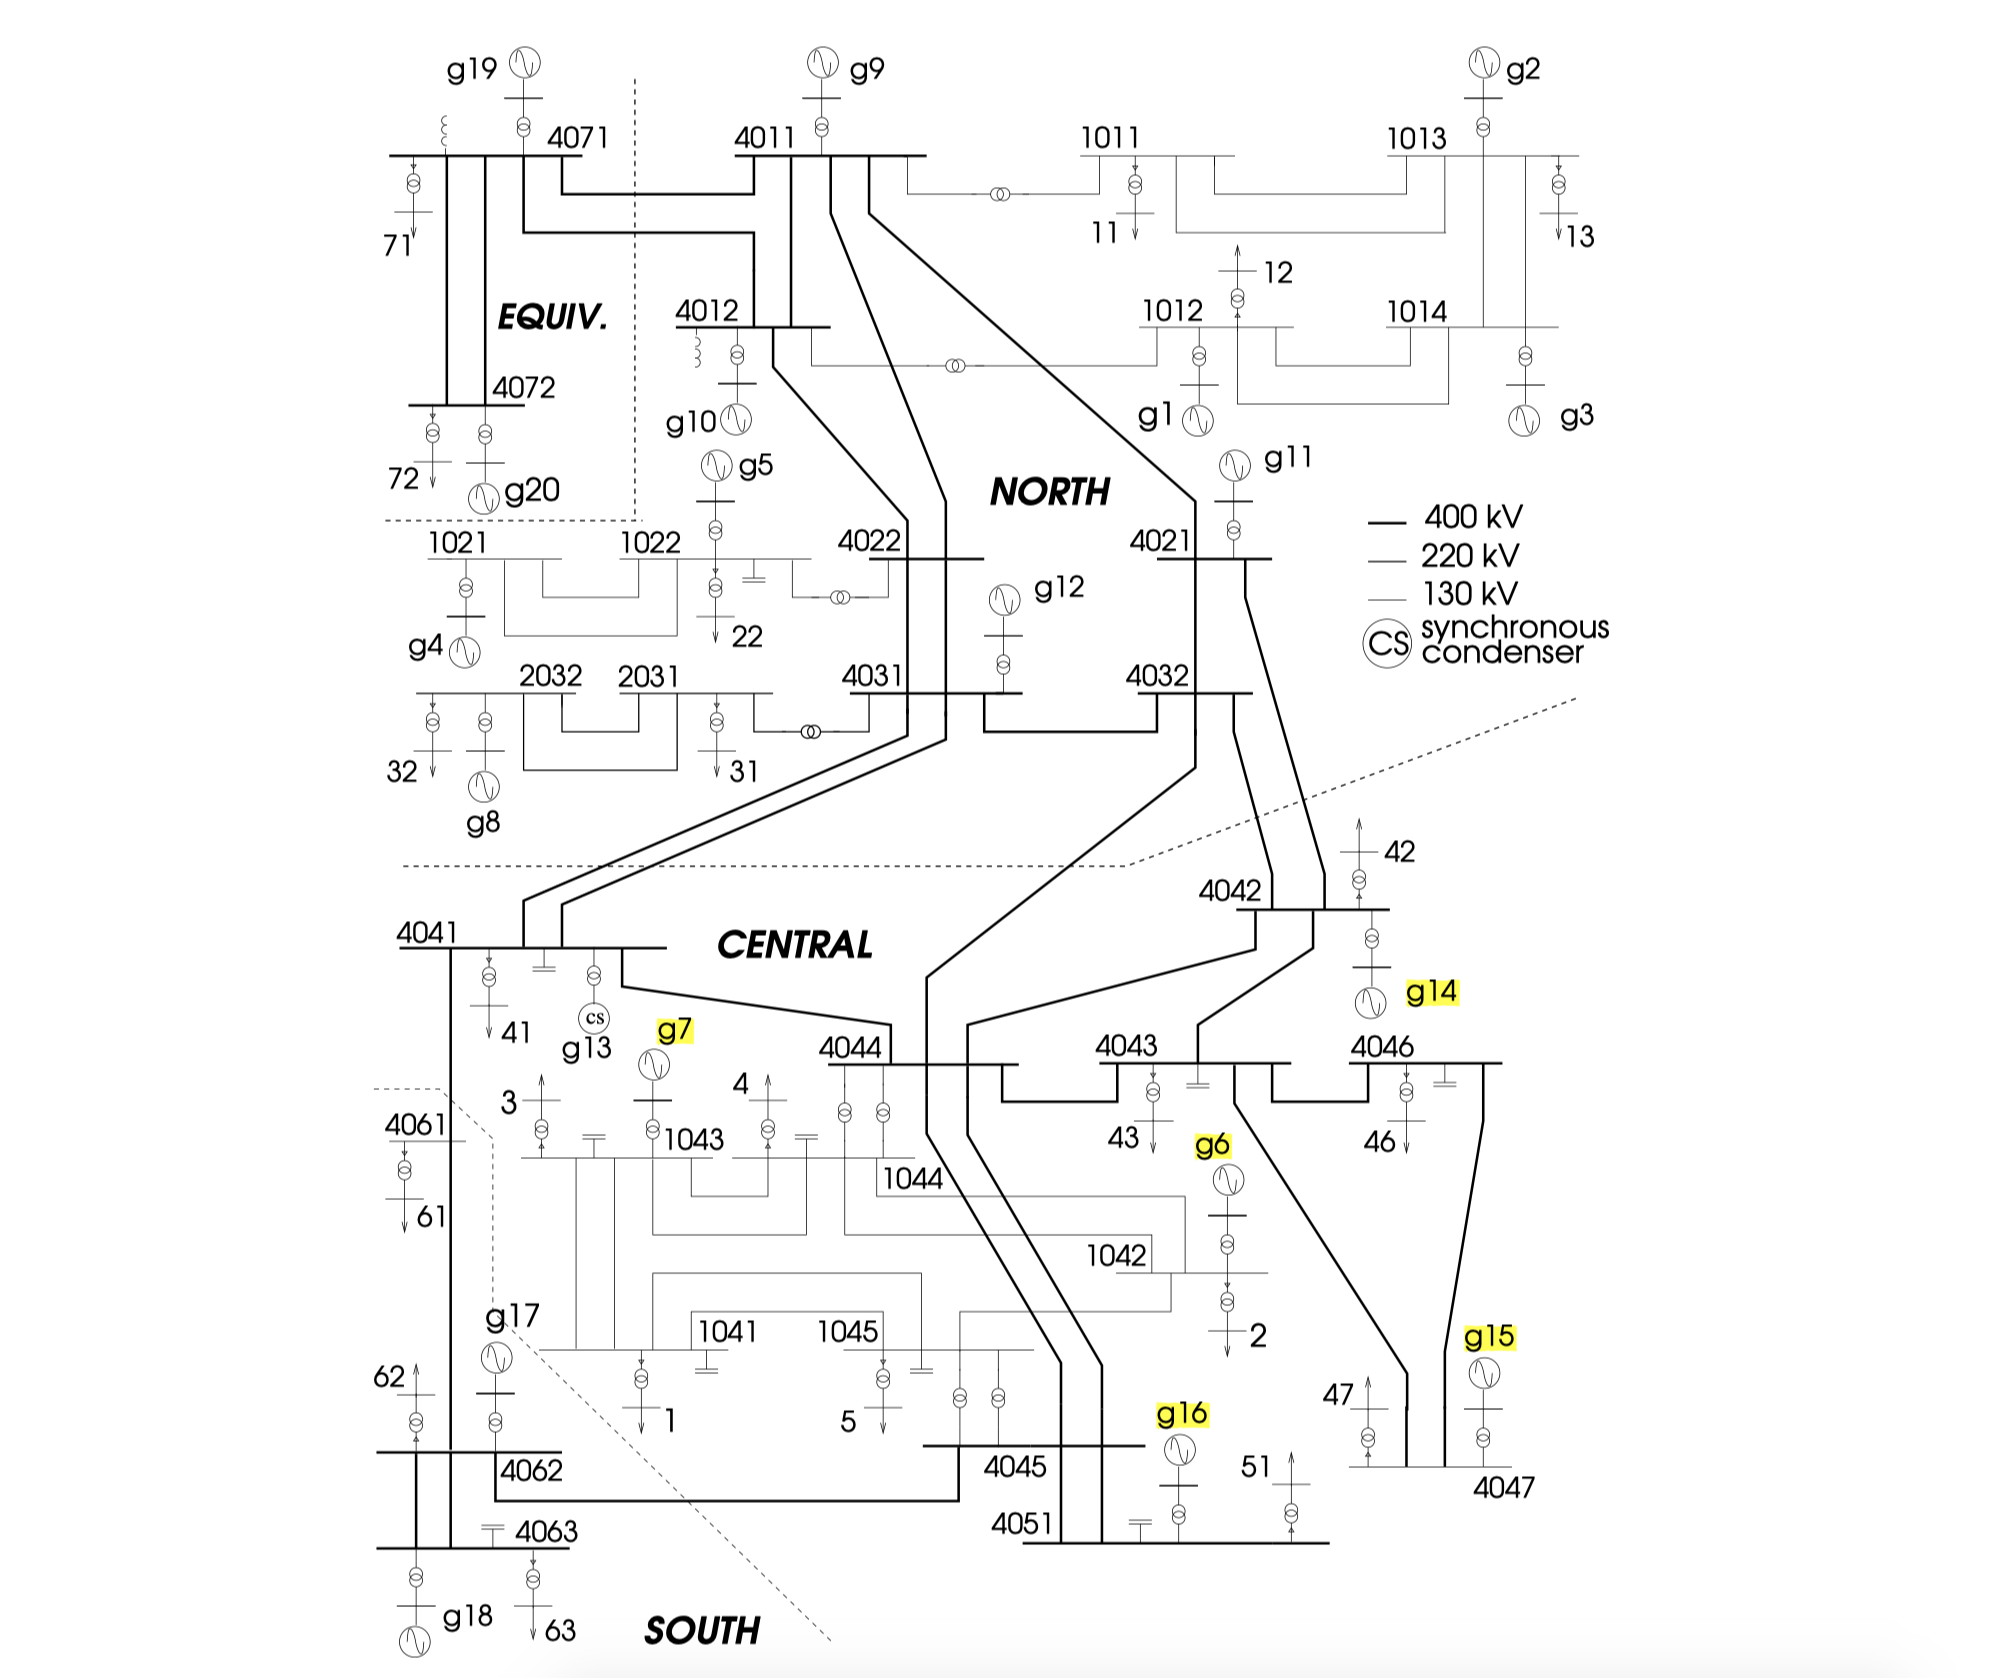
\includegraphics[width = \textwidth]{figure/4_1_1_nordic.png}
\caption{One-line diagram of the test system}
\label{4_1_1_nordic}
\end{figure}

Firstly, we assumed g2 as our monitor. The monitor will send its frequency, also the frequency in the system, to our communication layer. Then, we choose five thermal generators  (g6, g7, g14, g15, g16) in the CENTRAL area. There are three reasons I choose these five generators that produce the power to the system when disturbances occur in the system. First of all, these are thermal generators not the generators in the NORTH area which are equipped with hydraulic turbines. We only have strict mathematical proof of thermal generators. Another reason is they have nice nominal power as shown the Table \textcolor{red}{\ref{nominalPower}} below. The second reason is the difference of them is up to 900 MW which is good for researching the function of generators comprehensively. The last reason is I was collaborated with a PhD student. We researched Nordic test system in a different algorithm. He used distributed algorithm and I used centralised algorithm. For convenience, we keep our generators same.\\


\begin{table}[htbp]
\centering
\begin{tabular}{ll}
Generator & Nominal Power (MW) \\
g1        & 760.0              \\
g2        & 570.0              \\
g3        & 665.0              \\
g4        & 570.0              \\
g5        & 237.5              \\
g6        & 360.0 (1/8)        \\
g7        & 180.0 (1/16)       \\
g8        & 807.5              \\
g9        & 950.0              \\
g10       & 760.0              \\
g11       & 285.0              \\
g12       & 332.5              \\
g13       & 0.0                \\
g14       & 630.0 (7/32)       \\
g15       & 1080.0 (3/8)       \\
g16       & 630.0 (7/32)       \\
g17       & 540.0              \\
g18       & 1080.0             \\
g19       & 475.0              \\
g20       & 4275.0             

\end{tabular}
\label{nominalPower}
\caption{\label{tab:table-name}Generators Nominal Power in Nordic}
\end{table}

After choosing the generators, we need to choose a breaker. The breaker is a generator that will be disconnected to the system. Thus, a breaker is one of the most important impact factors to the grid system. However, I don’t know how to choose a suitable breaker at the beginning and then I try to disconnect them one boy one without Secondary Frequency Control. Results are as follows.\\

\begin{figure}[htbp]
\centering
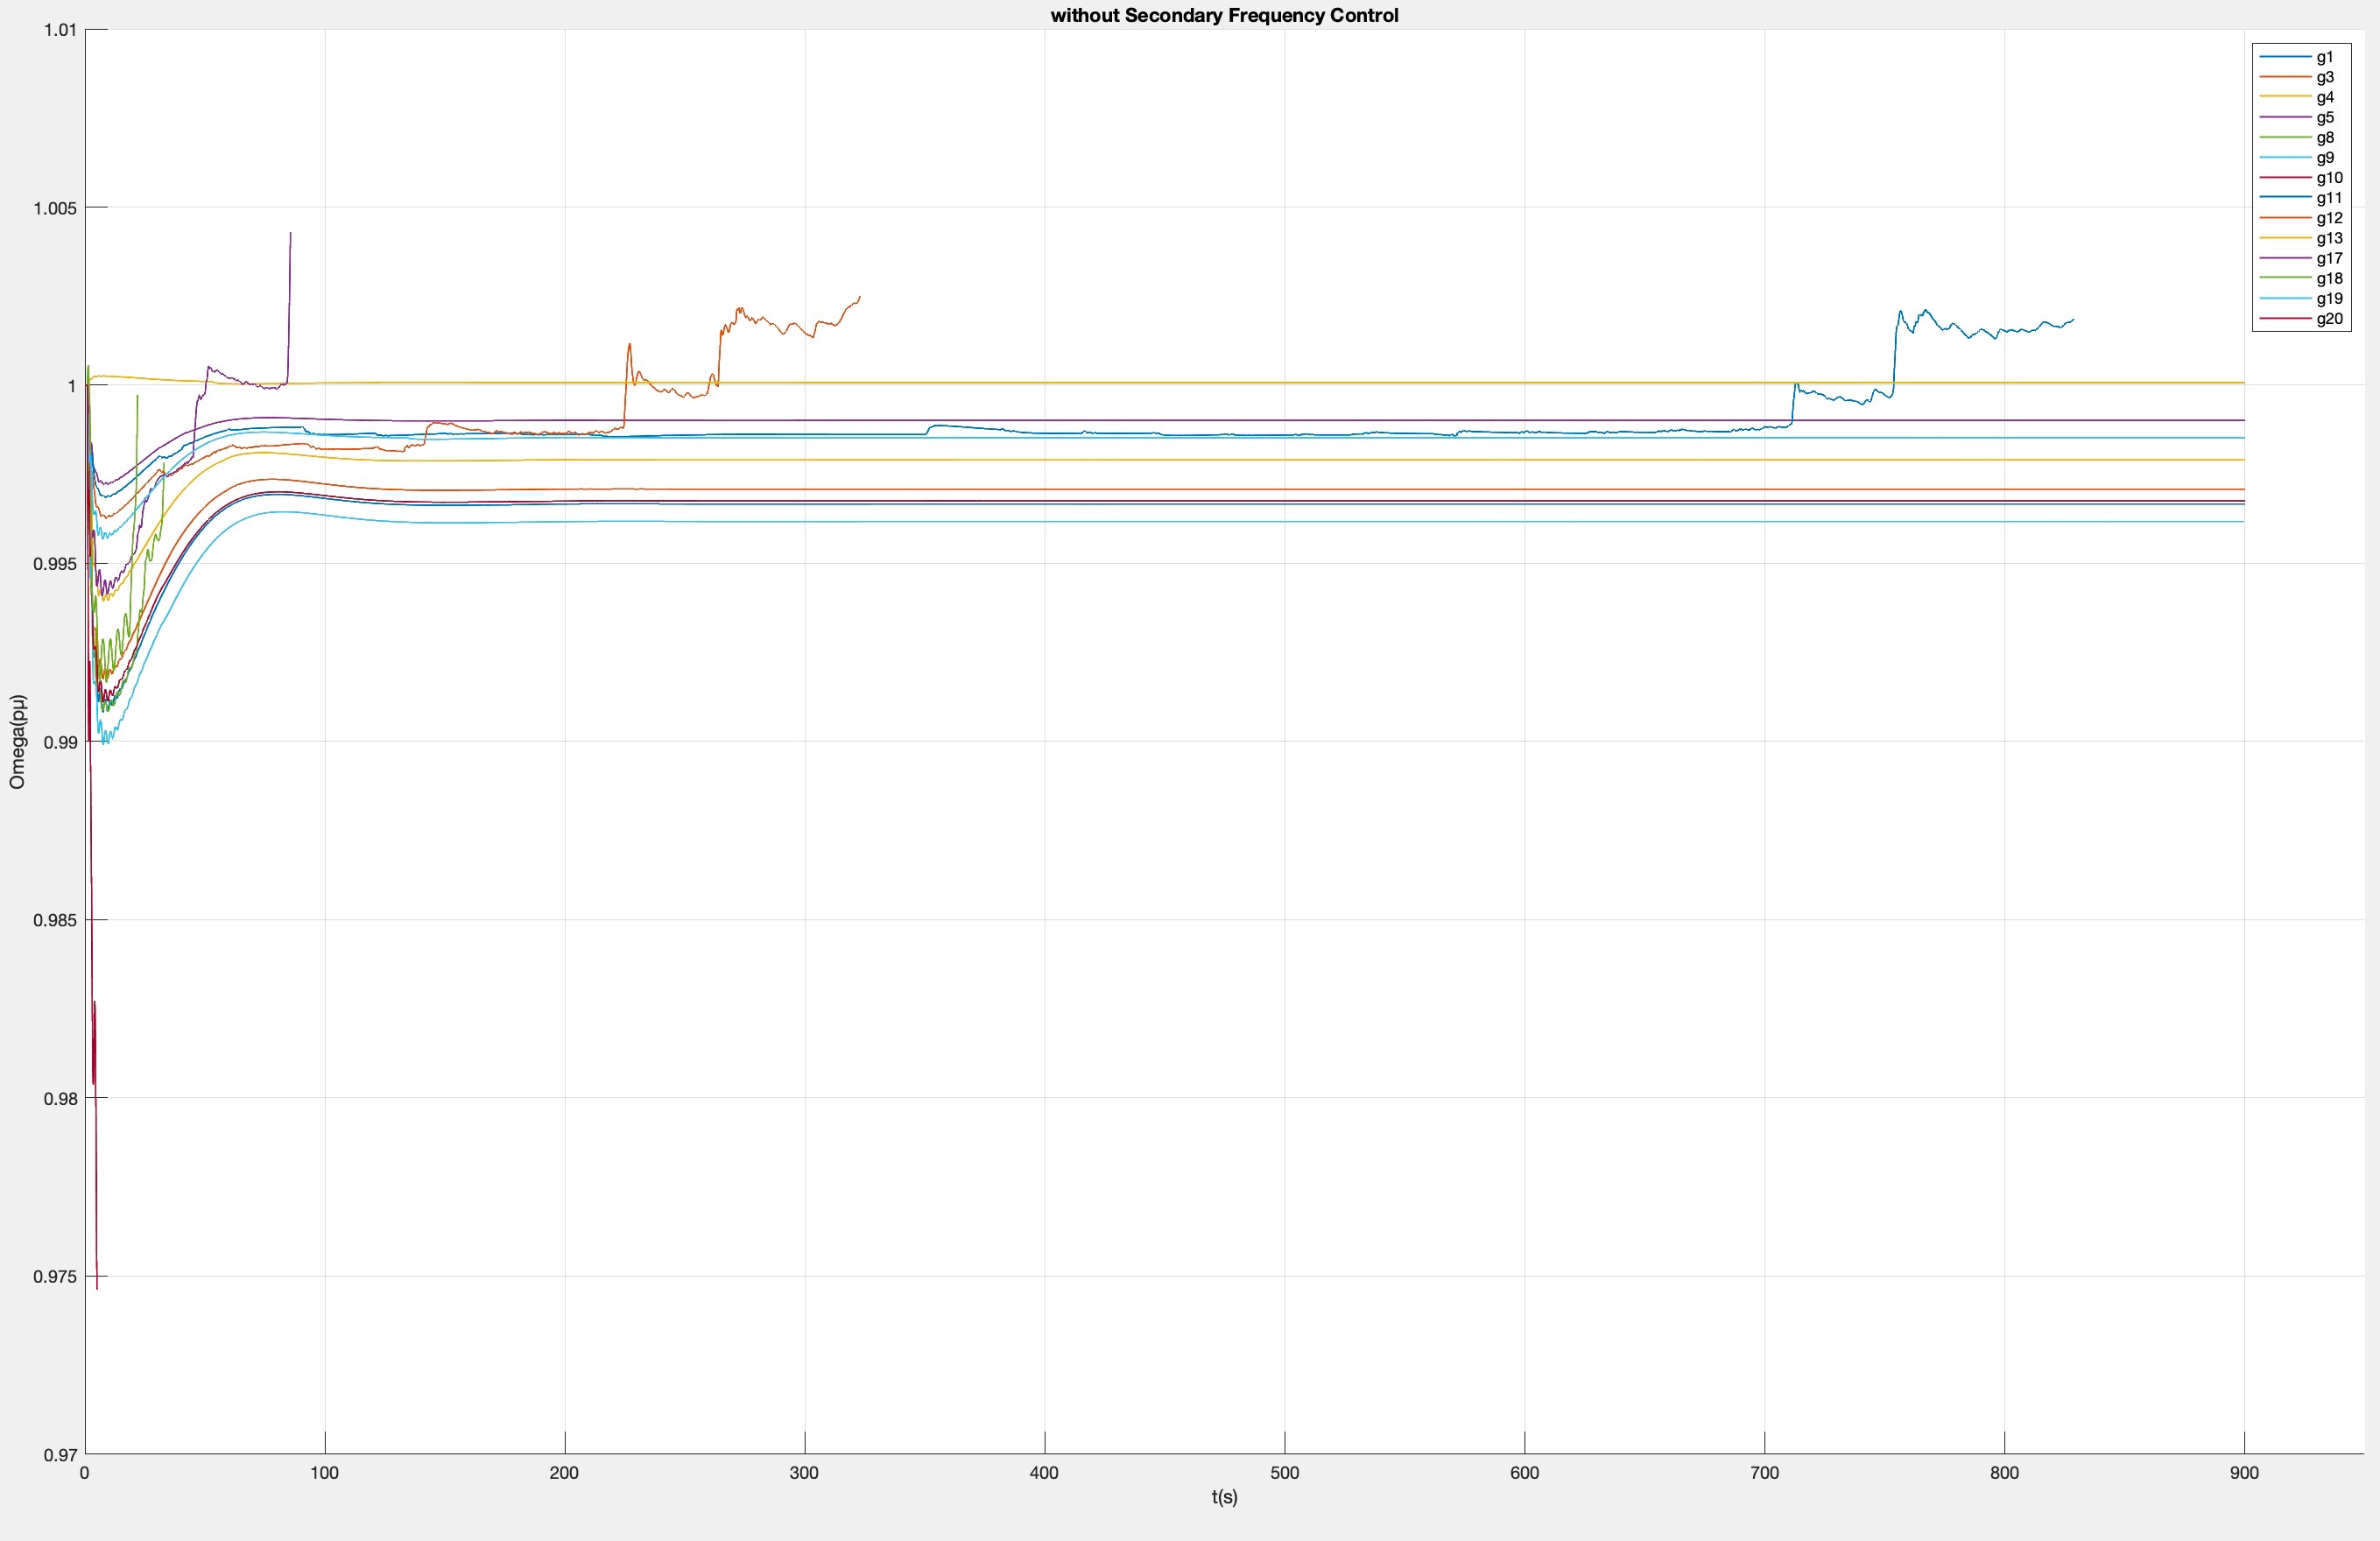
\includegraphics[width = \textwidth]{figure/4_1_1_without1.jpeg}
\caption{One-line diagram of the test system}
\label{4_1_1_without1}
\end{figure}

As we can see, g8, g17, g18 and g20 are extremely unstable before 100 seconds and g13 have zero nominal power. Thus, we will choose breaker out of them to make sure we have a smooth testing environment.\\


\begin{figure}[htbp]
\centering
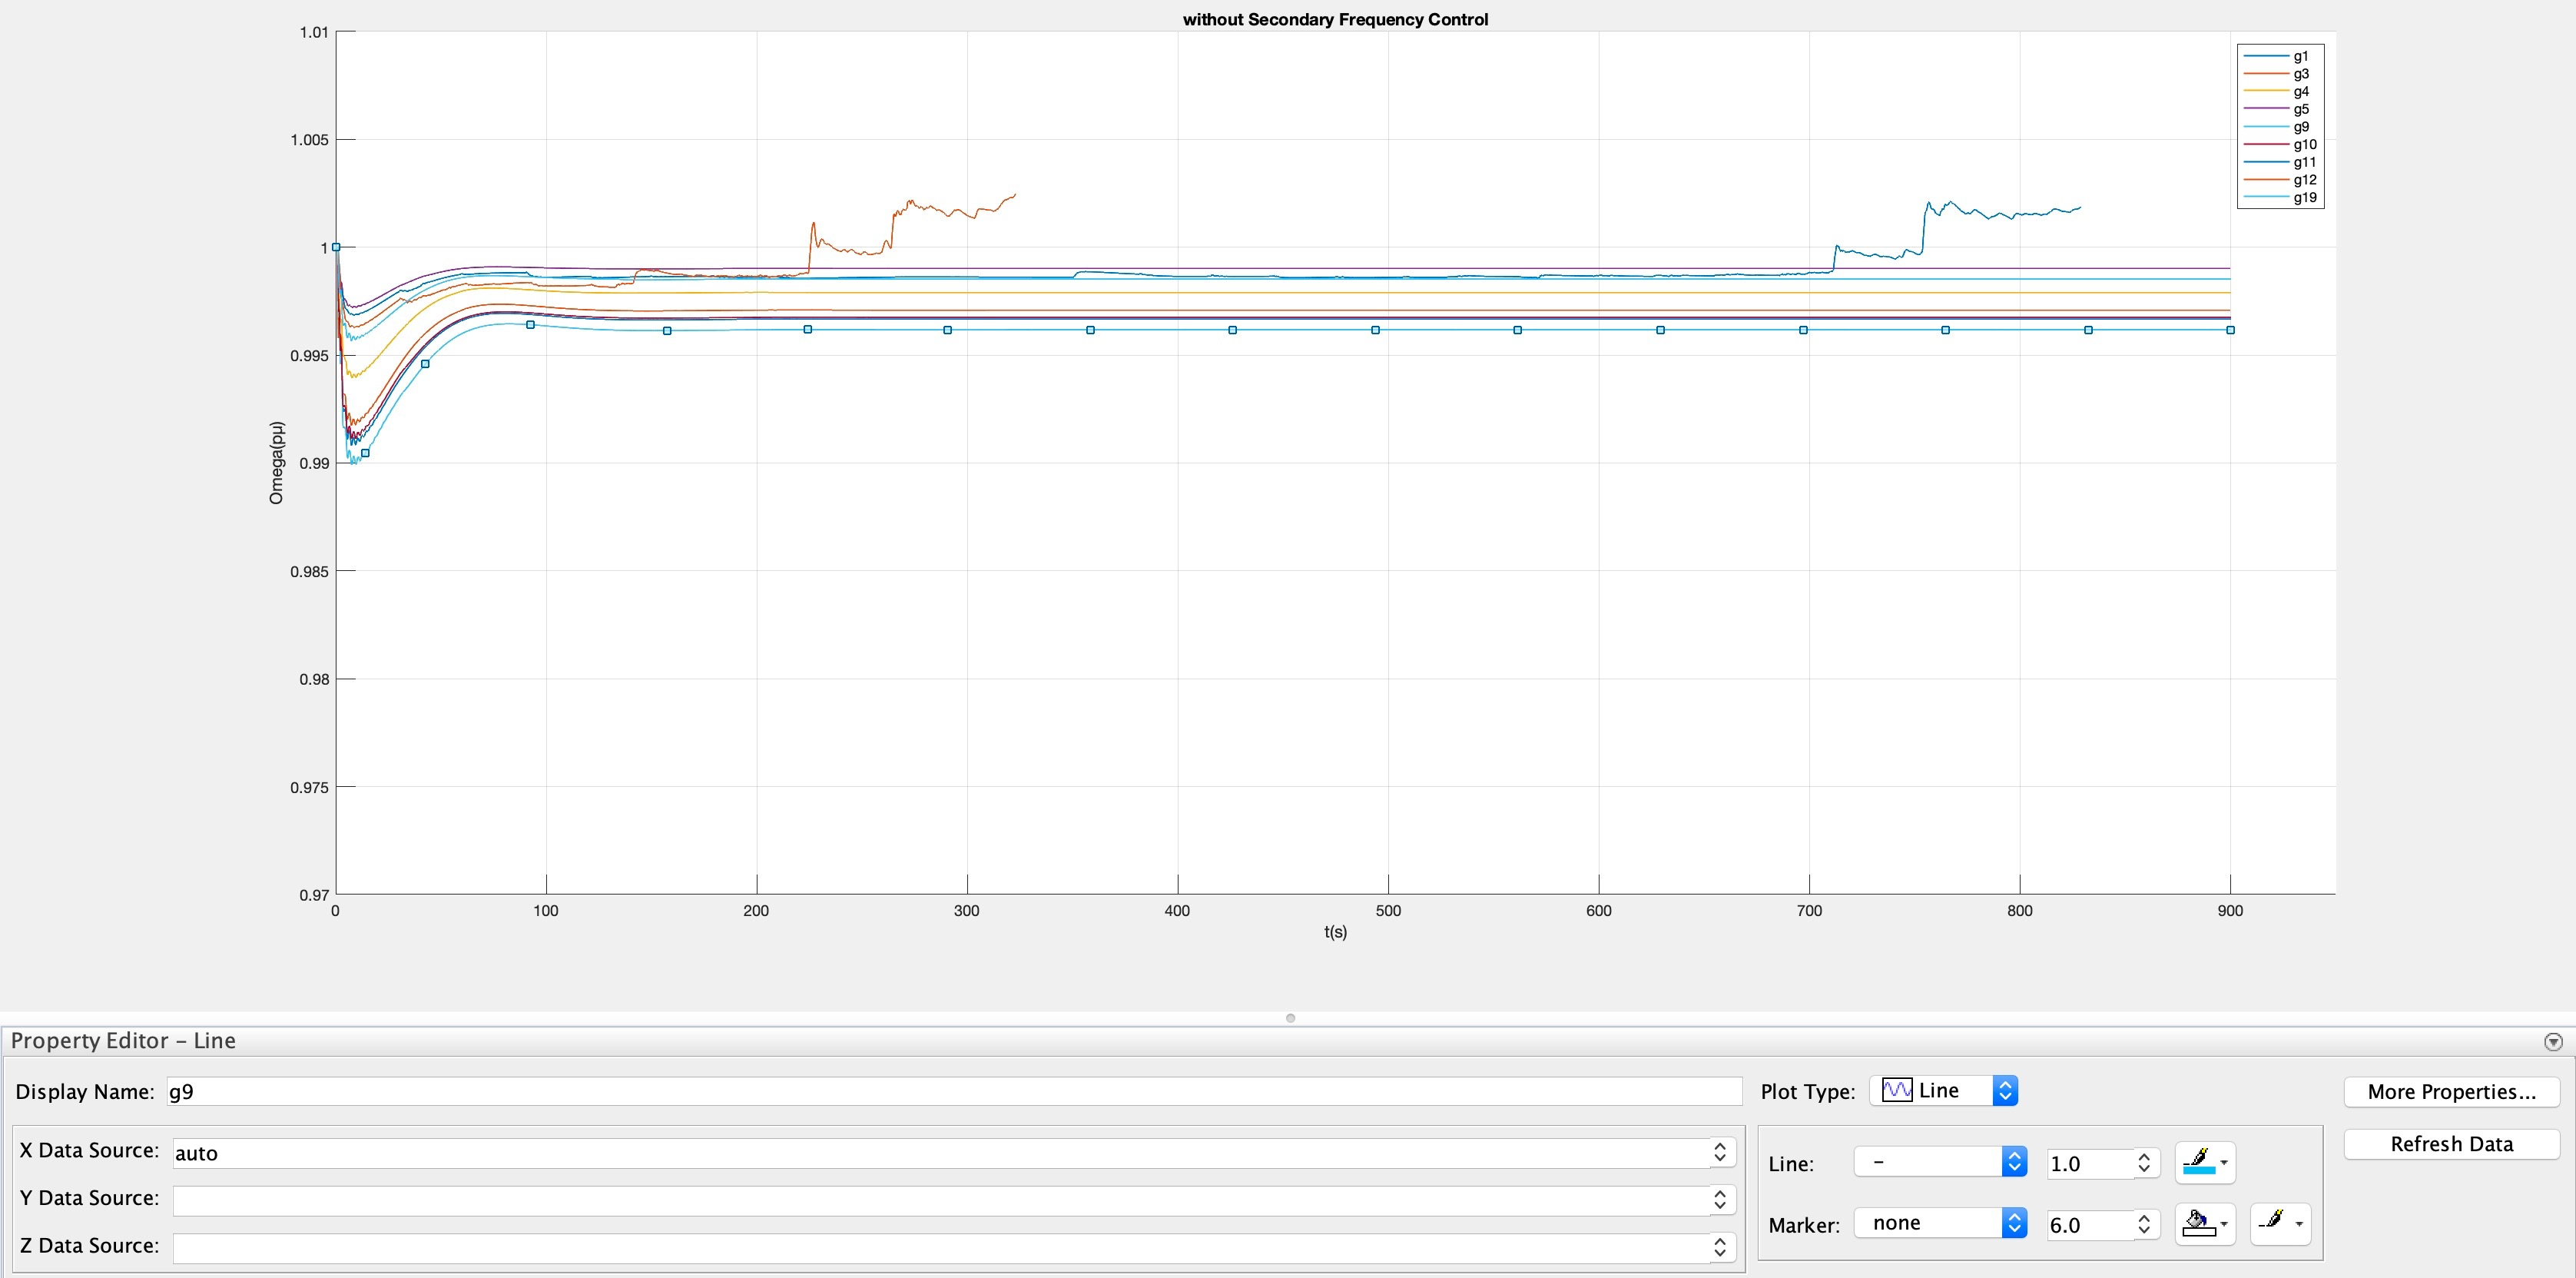
\includegraphics[width = \textwidth]{figure/4_1_1_without2.jpeg}
\caption{One-line diagram of the test system}
\label{4_1_1_without2}
\end{figure}

Finally, we choose g9 because it has a larger steady-state error. Thus, the turbines will send more power to the system. It is easier to see the change of kp and ki.\\\\\\\\

\subsection{Software Hypothesis} %4.1.2

\begin{figure}[htbp]
\centering
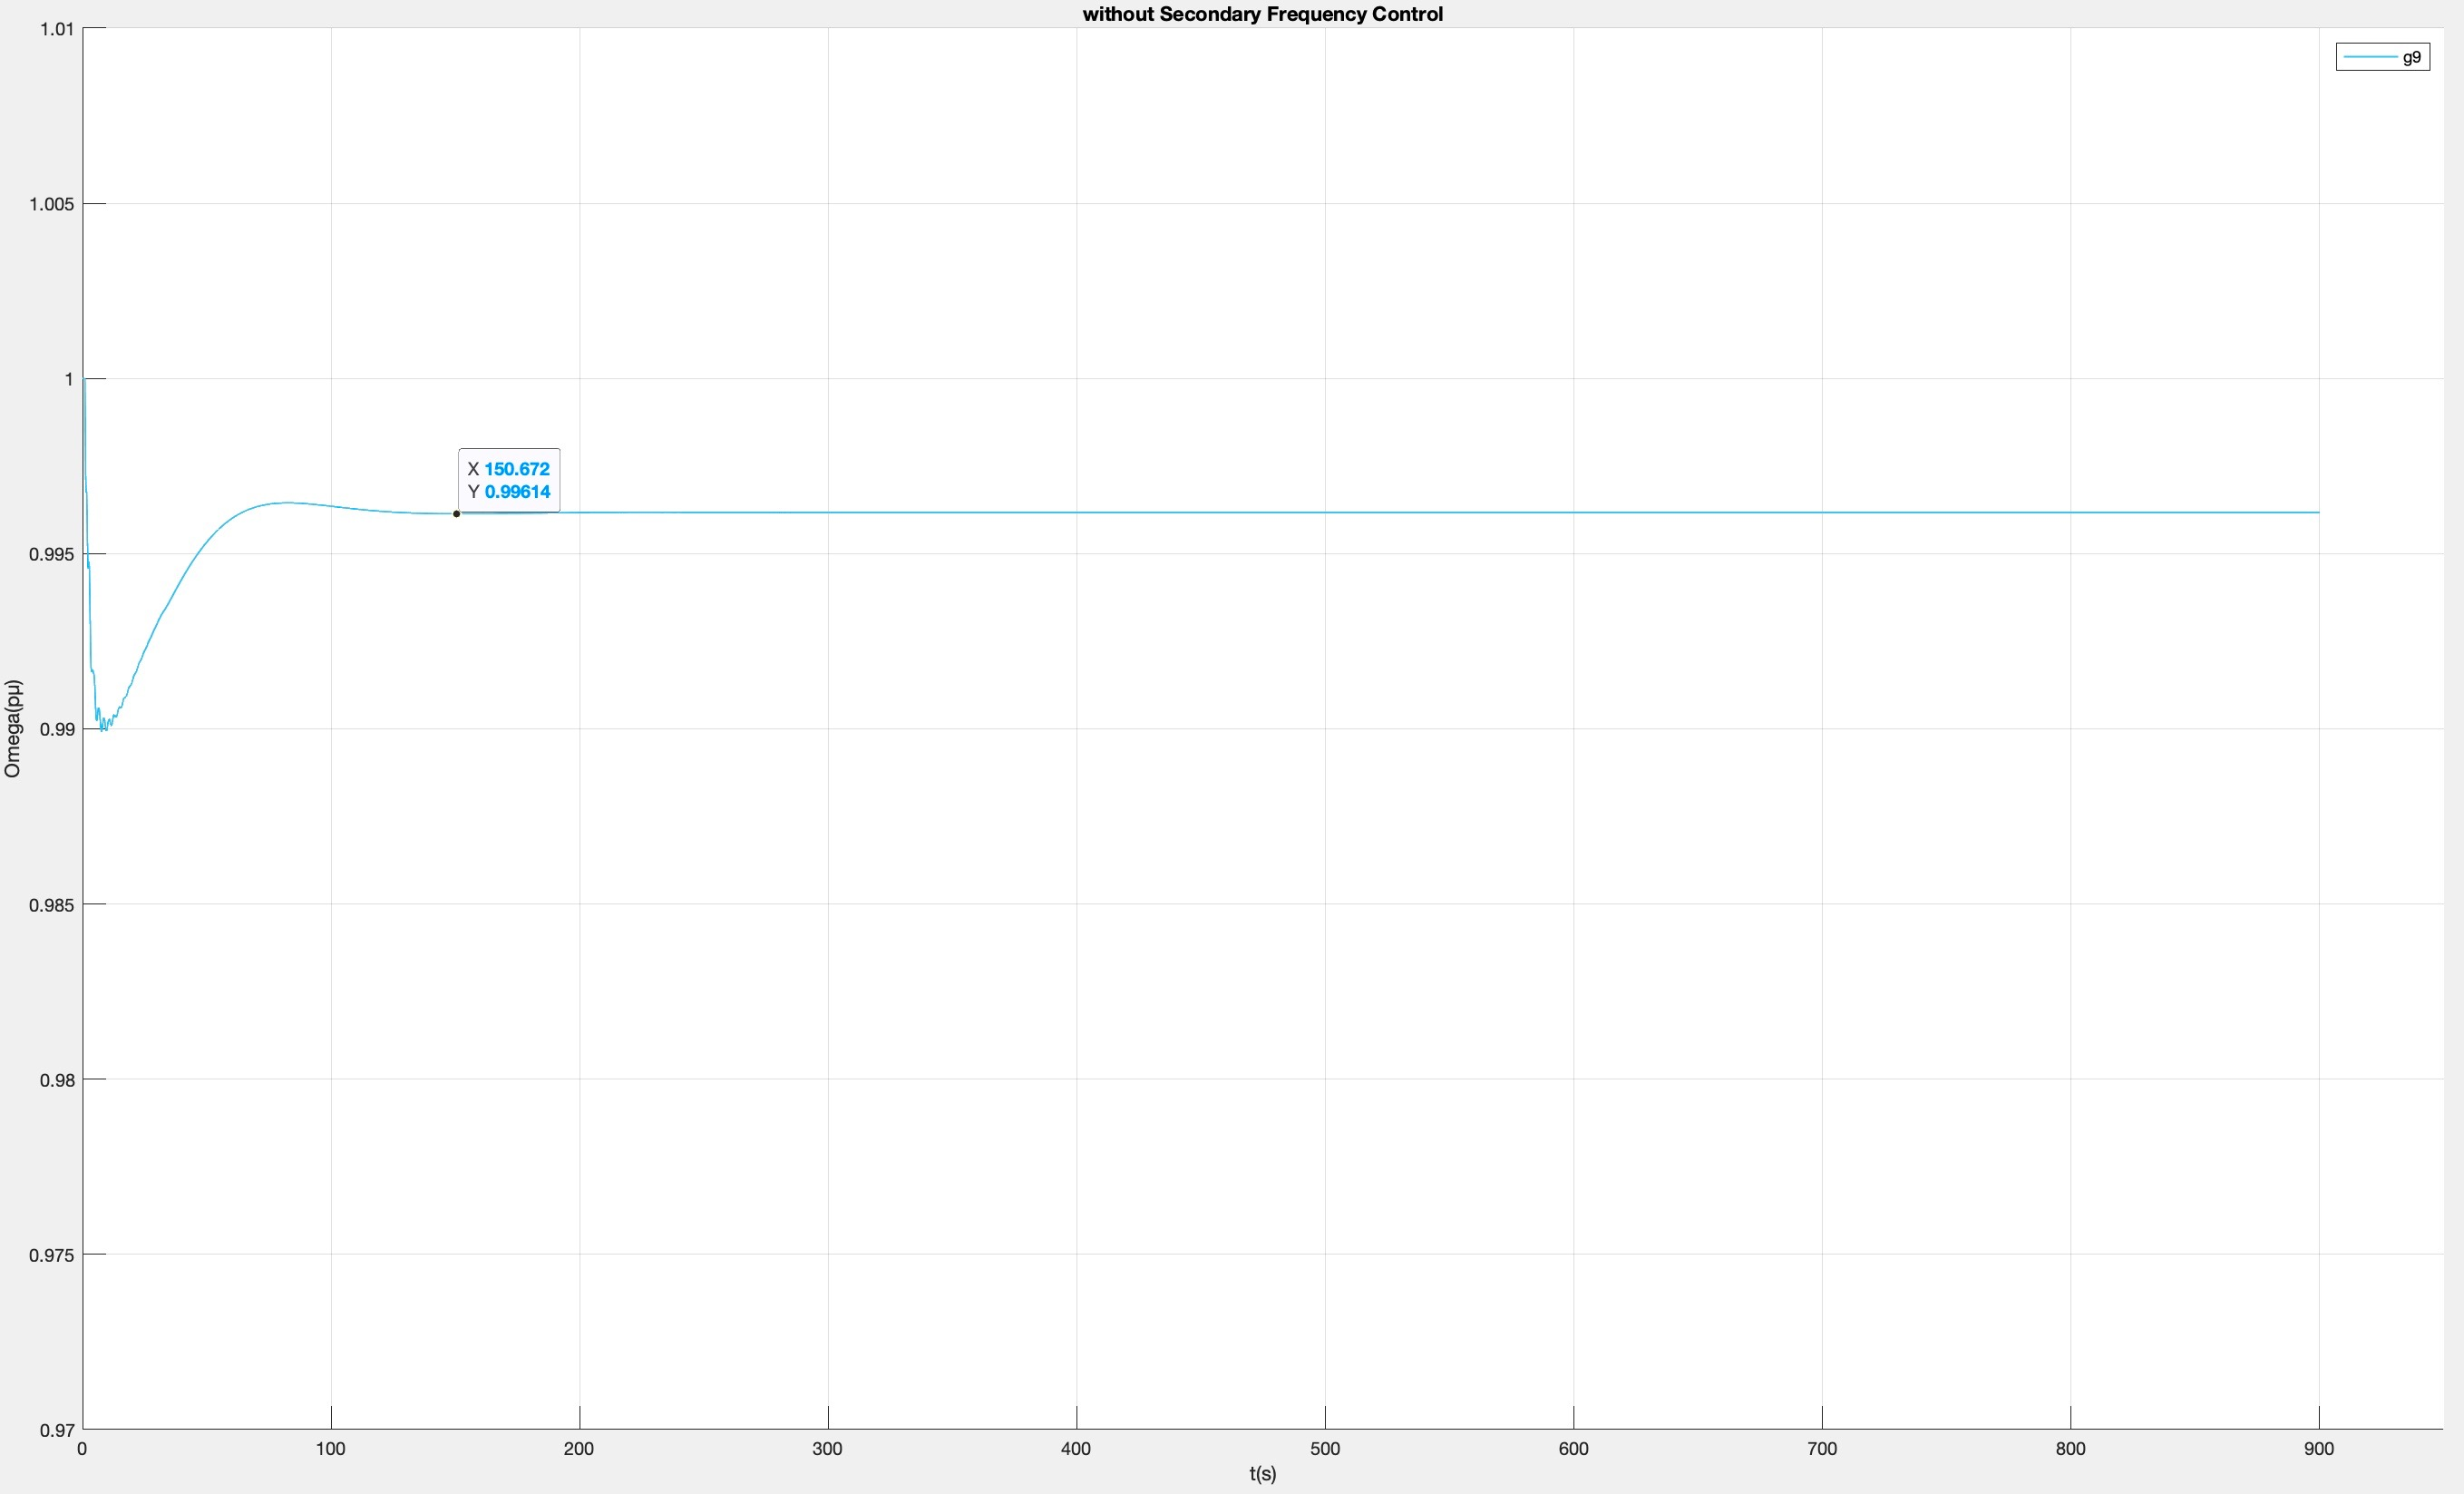
\includegraphics[width = \textwidth]{figure/4_1_1_without3.jpeg}
\caption{One-line diagram of the test system}
\label{4_1_1_without3}
\end{figure}
Next hypothesis is start time and end time. In the definition of Primary Frequency Control, its power balance will be restored at a lower or higher frequency, thus, from the Figure \textcolor{red}{\ref{4_1_1_without3}}, we can observe that, at t equals to 150 seconds, the power is in balance. Thus, I choose the 150th second at the beginning of Secondary Frequency Control. In the definition of Secondary Frequency Control, the response time of it will takes up to 15 minutes, thus, I choose the 900th second as my temporary end time.\\

Since it is a low time delay testing, we can assume that delay is 0.01 seconds. The reason for no choosing zero delay is that, in reality, there will be no such a zero delay scenario.\\

Next step, we need to start tuning kp and ki. Following the idea of section 3.4, firstly, we firstly assume a large value as the limit value of kp. Detailedly, we assume the range of kp and ki are both from 0.1 to 300.1 and their step are both 50. \\

Then, we use the designed MATLAB program to check whether the simulation results are acceptable. Detailedly, we set overshoot be smaller than 0.2 percent because it is required that the frequency error should be in range of ±0.1 Hz from the section 4.1.1 in the Nordic official document.\\

We also need to make sure the signal is really settled from 0.9998 to 1.0002 before the end time (i.e. the 900th second), thus, it is necessary to set the required setting time smaller than the end time. We set required settling time be 800 seconds. \\

Every signal will check if they are meet the settling criteria, i.e. the signal must be in a range of 0.9998 and 1.0002 at least from the 800th second.\\

Finally, the program will sketch the plots of all acceptable results and will give related information in the legends. \\

\begin{figure}[htbp]
\centering
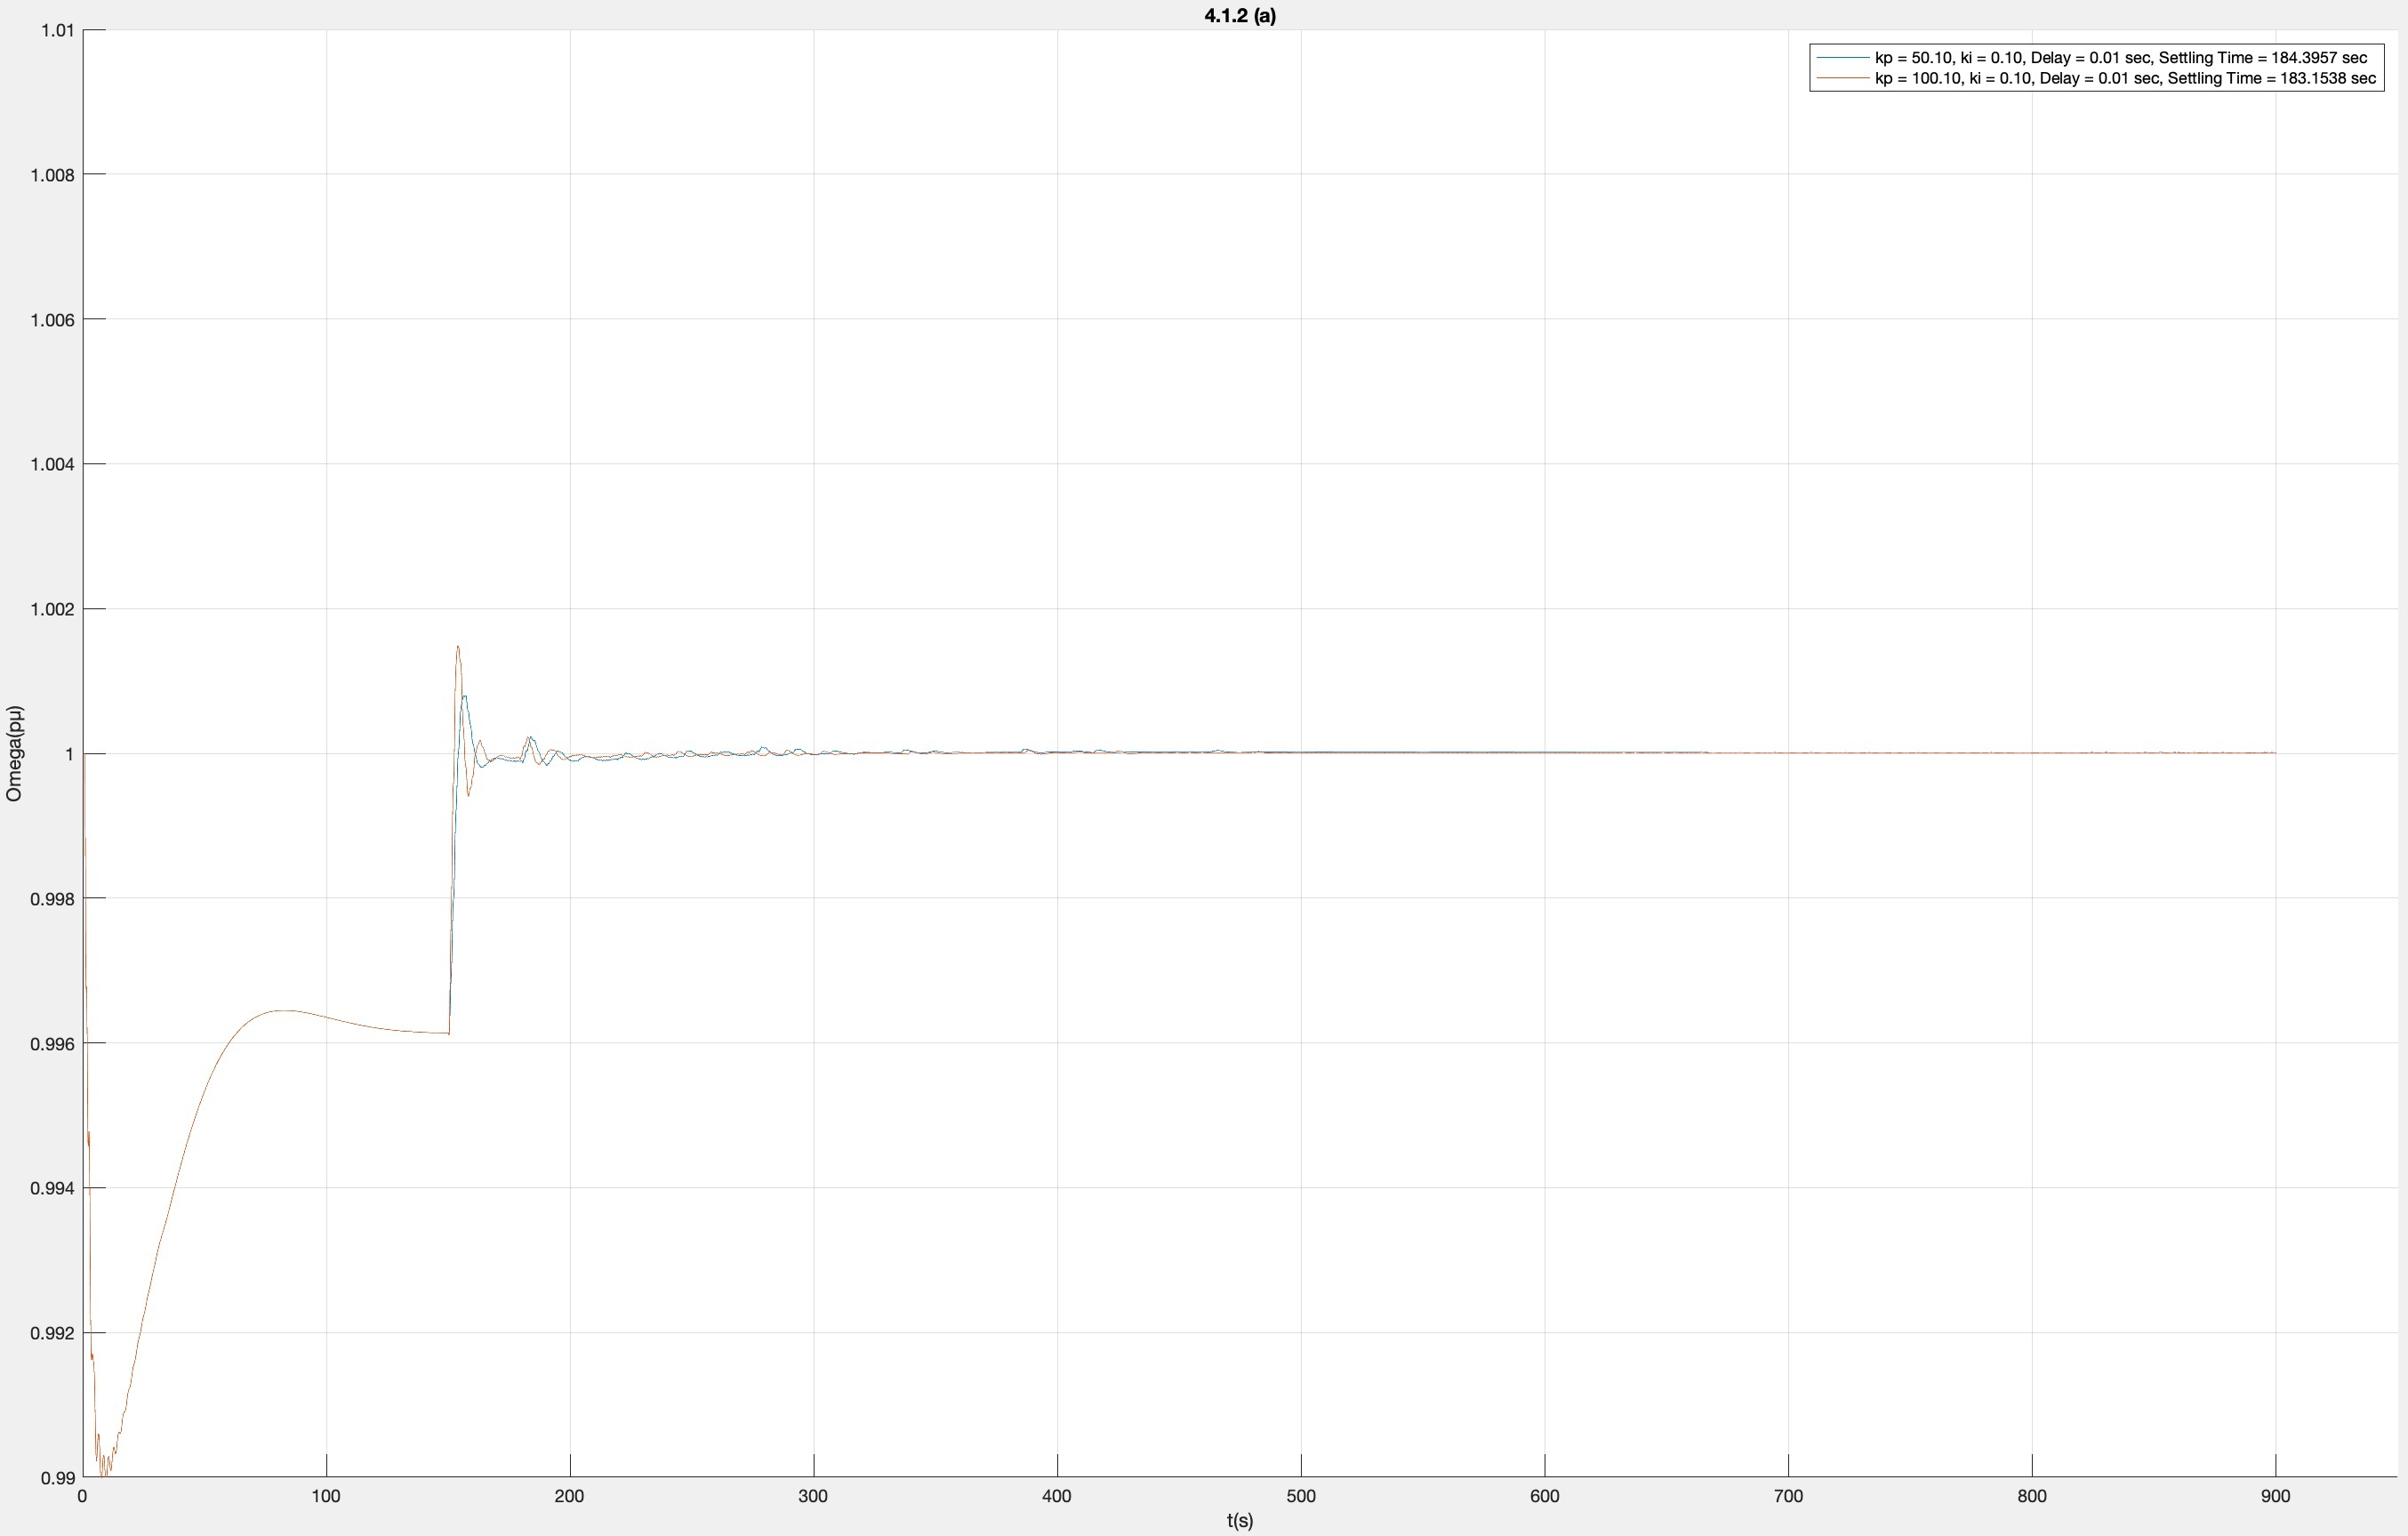
\includegraphics[width = \textwidth]{figure/4_1_1_a.jpeg}
\caption{One-line diagram of the test system}
\label{4_1_1_a}
\end{figure}

However, as you can see from Figure \textcolor{red}{\ref{4_1_1_a}}, only two of all the simulations are acceptable. The maximum value of kp is 100.1 and the maximum value of ki is 0.1. \\

According to the regulations from the last Chapter, we need to increase the maximum amplifier factor by the step value. \\

For instance, the new range of kp is between 0.1 and 150.1 and the new range of ki is between 0.1 and 50.1. To make a more accurate result, we need to decrease the step at the same time. We set step to 10.0. \\

Finally, we will have another plot as shown in Figure \textcolor{red}{\ref{4_1_1_b}}. \\

\begin{figure}[htbp]
\centering
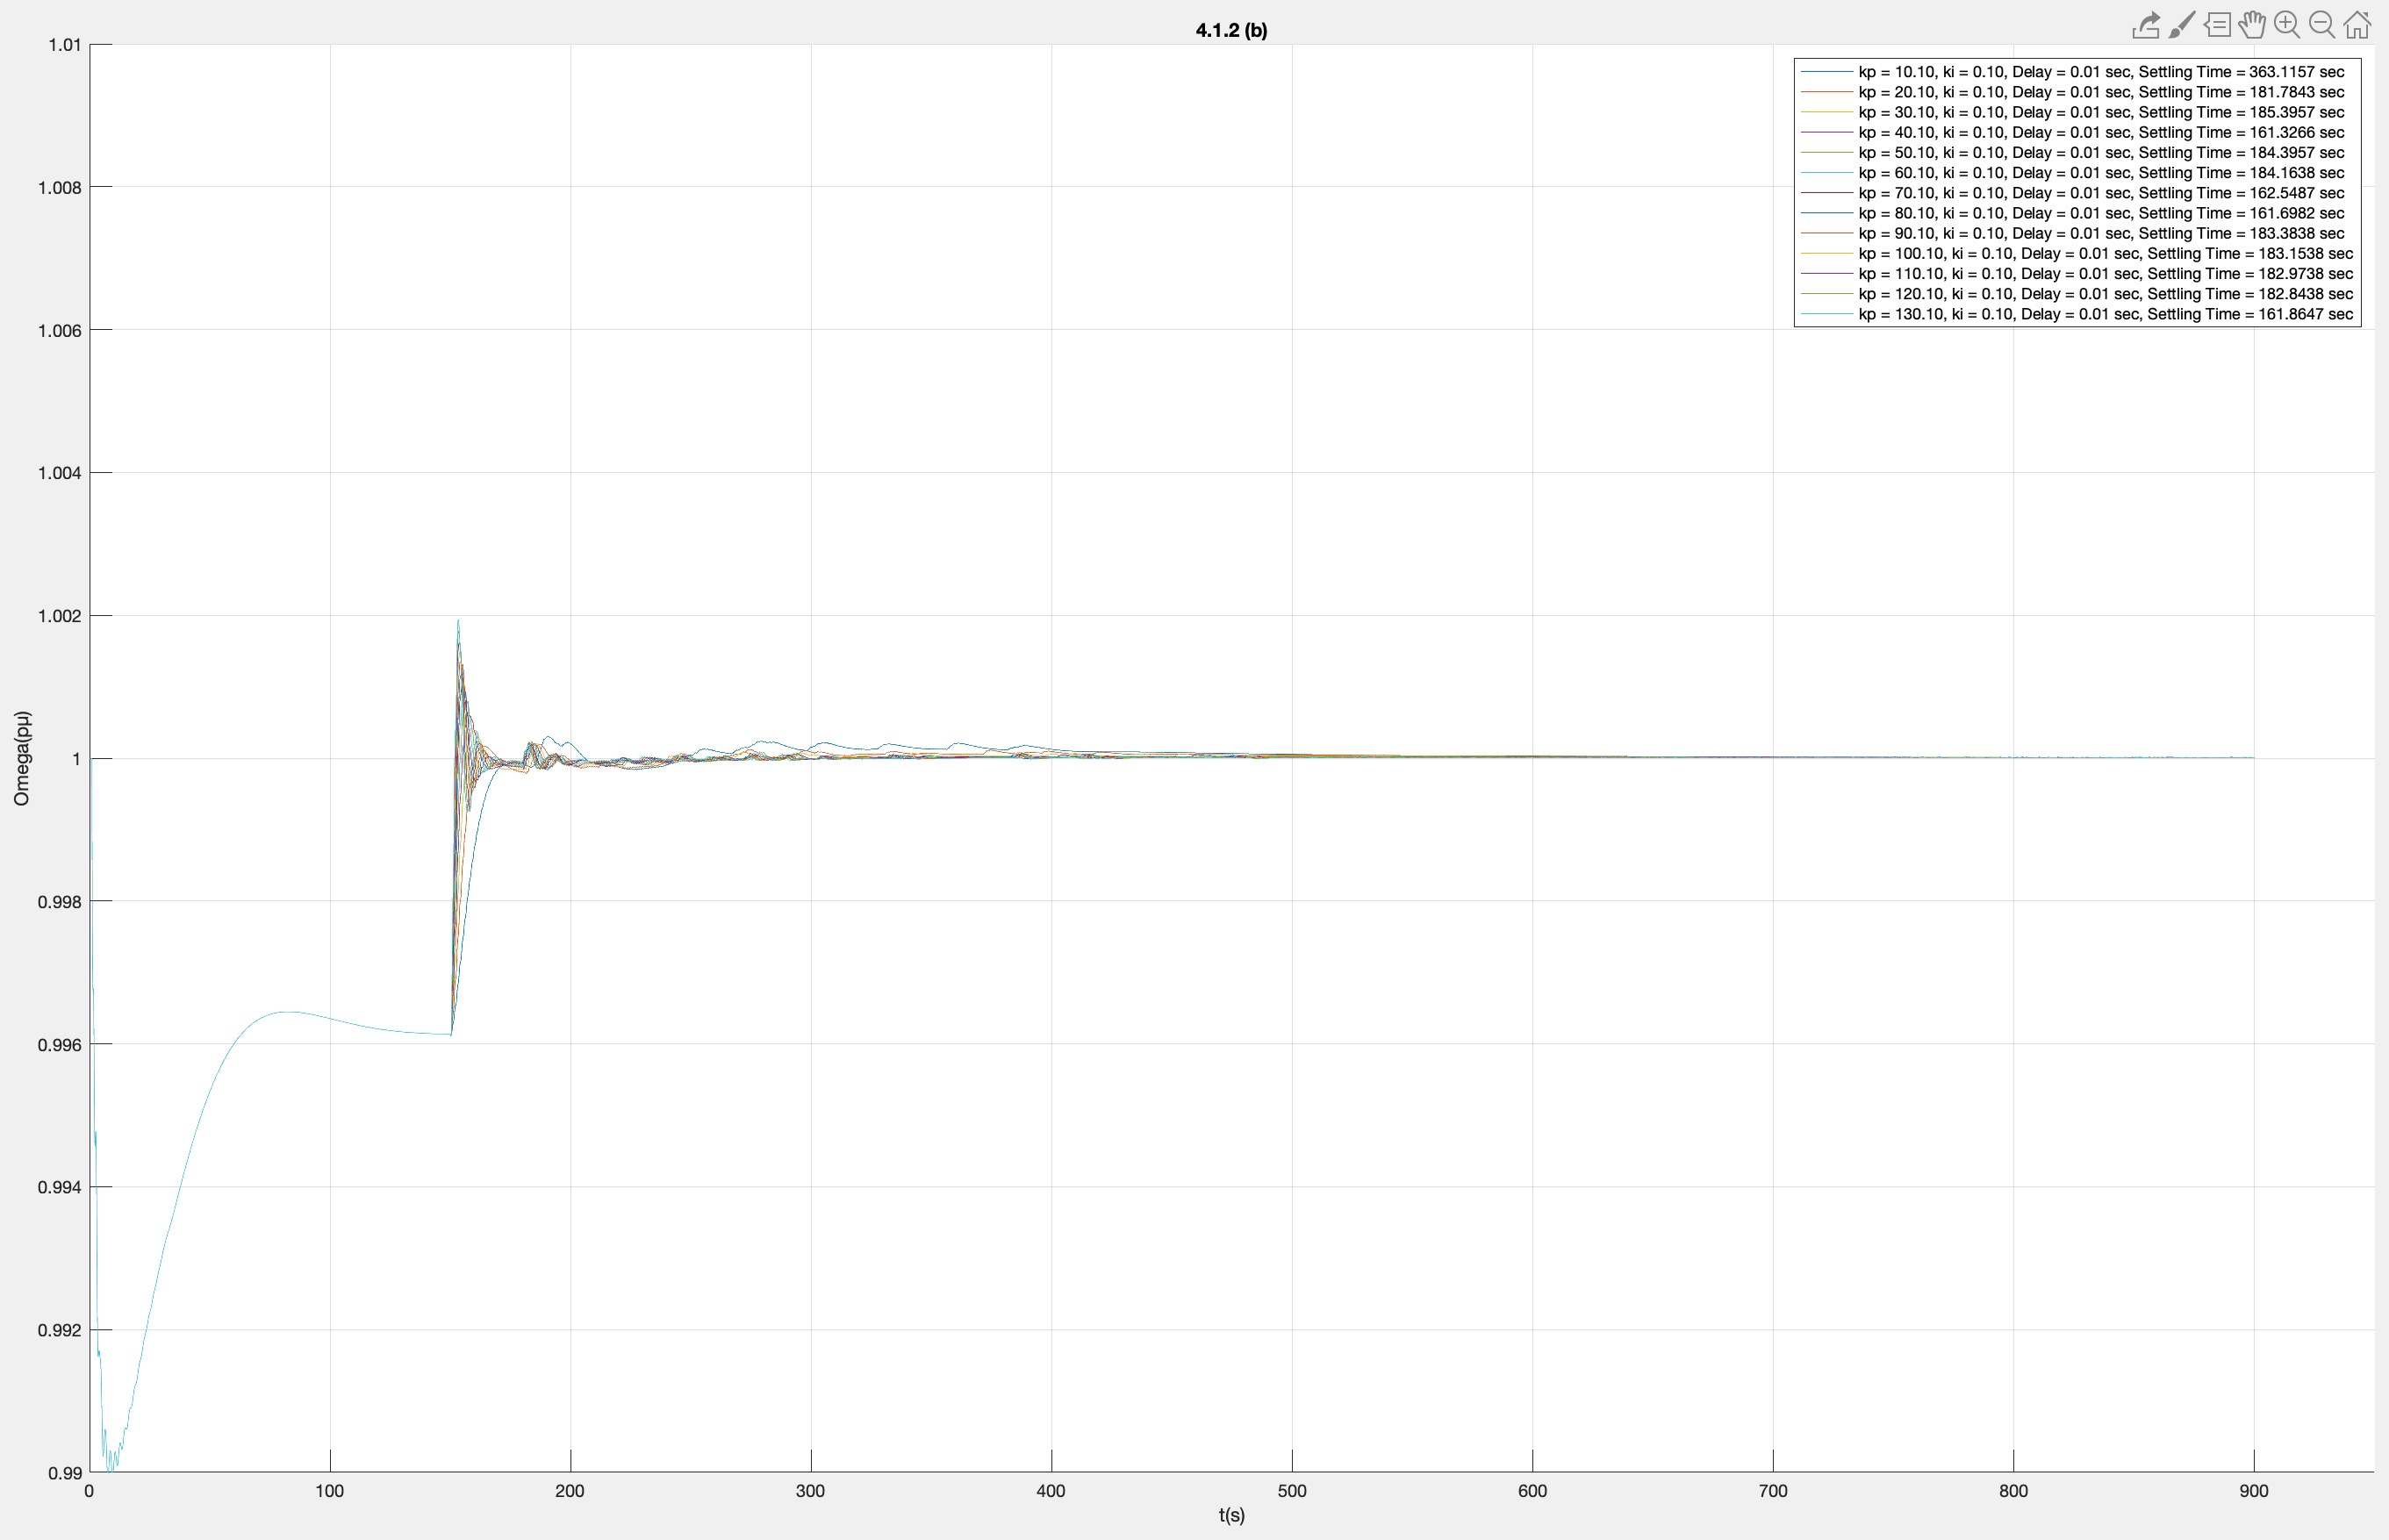
\includegraphics[width = \textwidth]{figure/4_1_1_b.jpeg}
\caption{One-line diagram of the test system}
\label{4_1_1_b}
\end{figure}


Apparently, we have more acceptable results than last simulation because of shrinking the step of kp. We can find that the simulations are unacceptable if kp equals to 140.1 or 150.1. Thus, we can finally fix the range of kp between 0.1 and 140.1 and keep the step of kp to 10. \\

We could set ki in a range of 0.1 and 10.1 with the reason above. However, it is possible the maximum value of ki is still 0.1 if we set the range of ki be from 0.1 and 10.1. Then the simulations are meaningless. \\

Thus, we need to apply bisection method on the rang of ki and find the meaningful maximum ki. Detailedly, we range kp from 0.1 to 140.1 and its step is 10.0. We set ki equals to 5.1. The purpose of doing this is to find if there are acceptable results if ki is in the middle of 0.1 and 10.1.\\   

The filtered results are as Figure \textcolor{red}{\ref{4_1_1_c}}. \\

\begin{figure}[htbp]
\centering
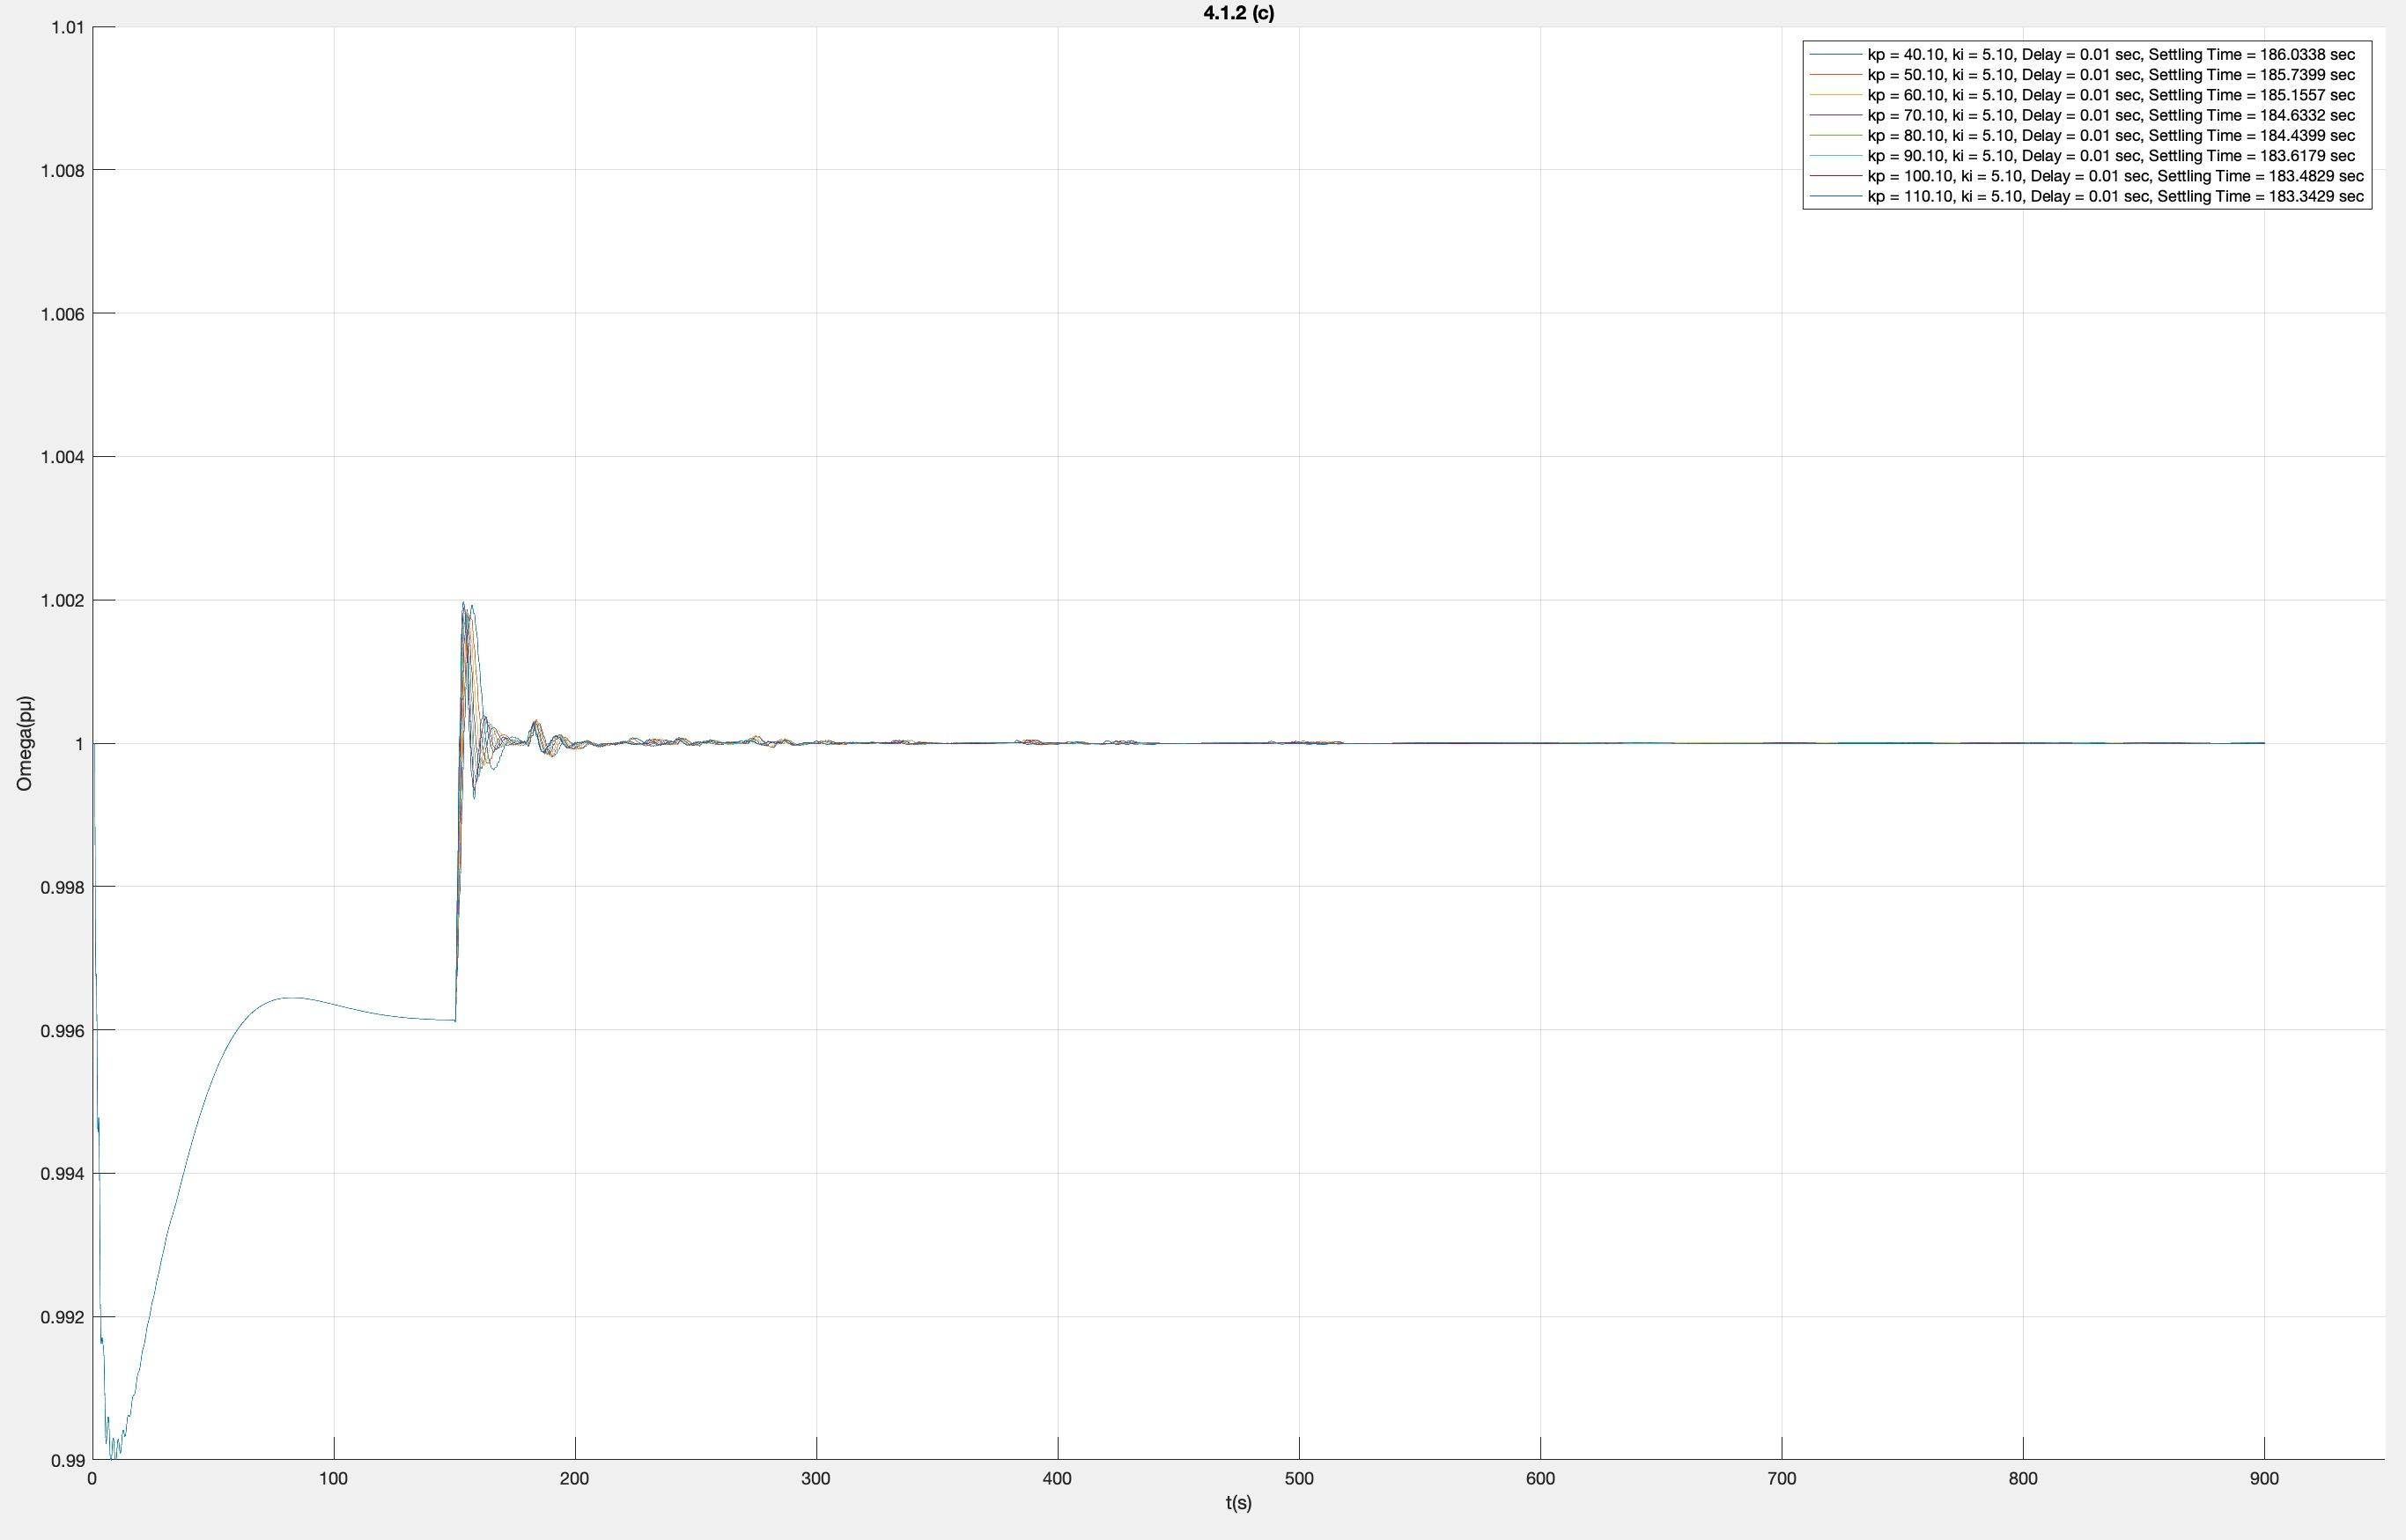
\includegraphics[width = \textwidth]{figure/4_1_1_c.jpeg}
\caption{One-line diagram of the test system}
\label{4_1_1_c}
\end{figure}

The results shows there are acceptable simulations if ki equals to 5.1. \\

Thus, we can set the range of ki between 0.1 and 10.1. 
Besides, we can reset the end time to 240 seconds and the required settling time to 200 seconds since most of the acceptable settling time are smaller than 200 seconds.\\

\section{Expected Outcome} %4.2
From discussions before, we know that both kp and ki can not be expanded indefinitely since we have specialised limit for kp and ki in MATLAB program. Thus, firstly, I hope to see a clearly borderline to separate the acceptable results and unacceptable results. The acceptable results will be expressed as blue points in Excel. \\

Secondly, I hope to see a relationship between the best point, which has minimum settling time among all the acceptable results, and other acceptable points. I expect the best point will not in the borderline because the points are unstable in the borderline. \\

I also do not hope the best point has a large or small kp and ki. A larger kp will produce a larger overshoot although it will be relative faster. A small kp has a larger probability of producing a steady-state error and it will be relative harder to approach a settled statement. A larger ki produces more oscillations, like Figure \textcolor{red}{\ref{3_4_1_larger_ki}} shown. It is also not easy to approach a settled statement. A small ki will not help fixing the steady-state error along with a small kp. \\


\section{Implement} %4.3
One of the most important idea to implement the testing is modularizing the function. We modularize our functions, like the AGC algorithm, the moving file script and ending file script, in a python file so we can import them as a library and call them in the main file directly. Additionally, it is necessary to remove hard coded parameters so it is easy to change the parameters like start time, end time, prepared folder address and list of generators in the main function.\\

Another noteworthy detail is we need to keep two significant digits for kp, ki and time delay. It provides a unified format that will help exporting data into analytical algorithms.\\

\begin{figure}[htbp]
\centering
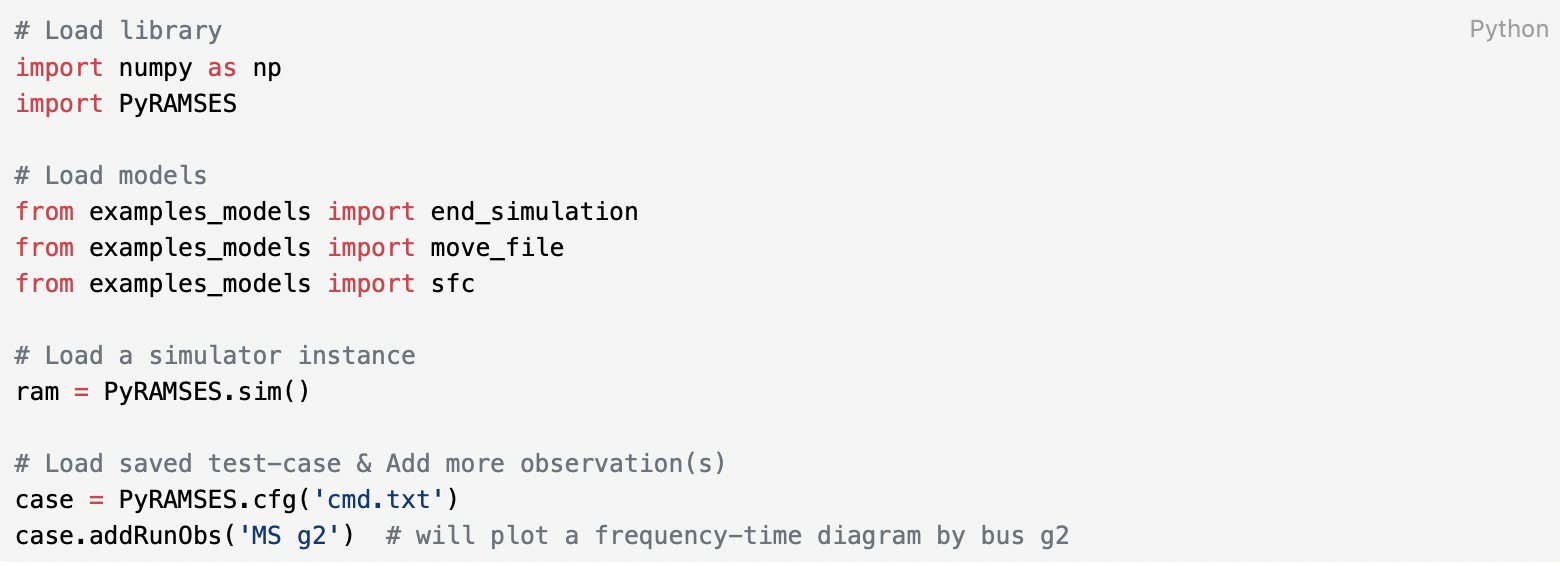
\includegraphics[width = \textwidth]{figure/4_3_code1.png}
%\caption{ }
\label{4_3_code1}
\end{figure}

\begin{figure}[hbtp]
\centering
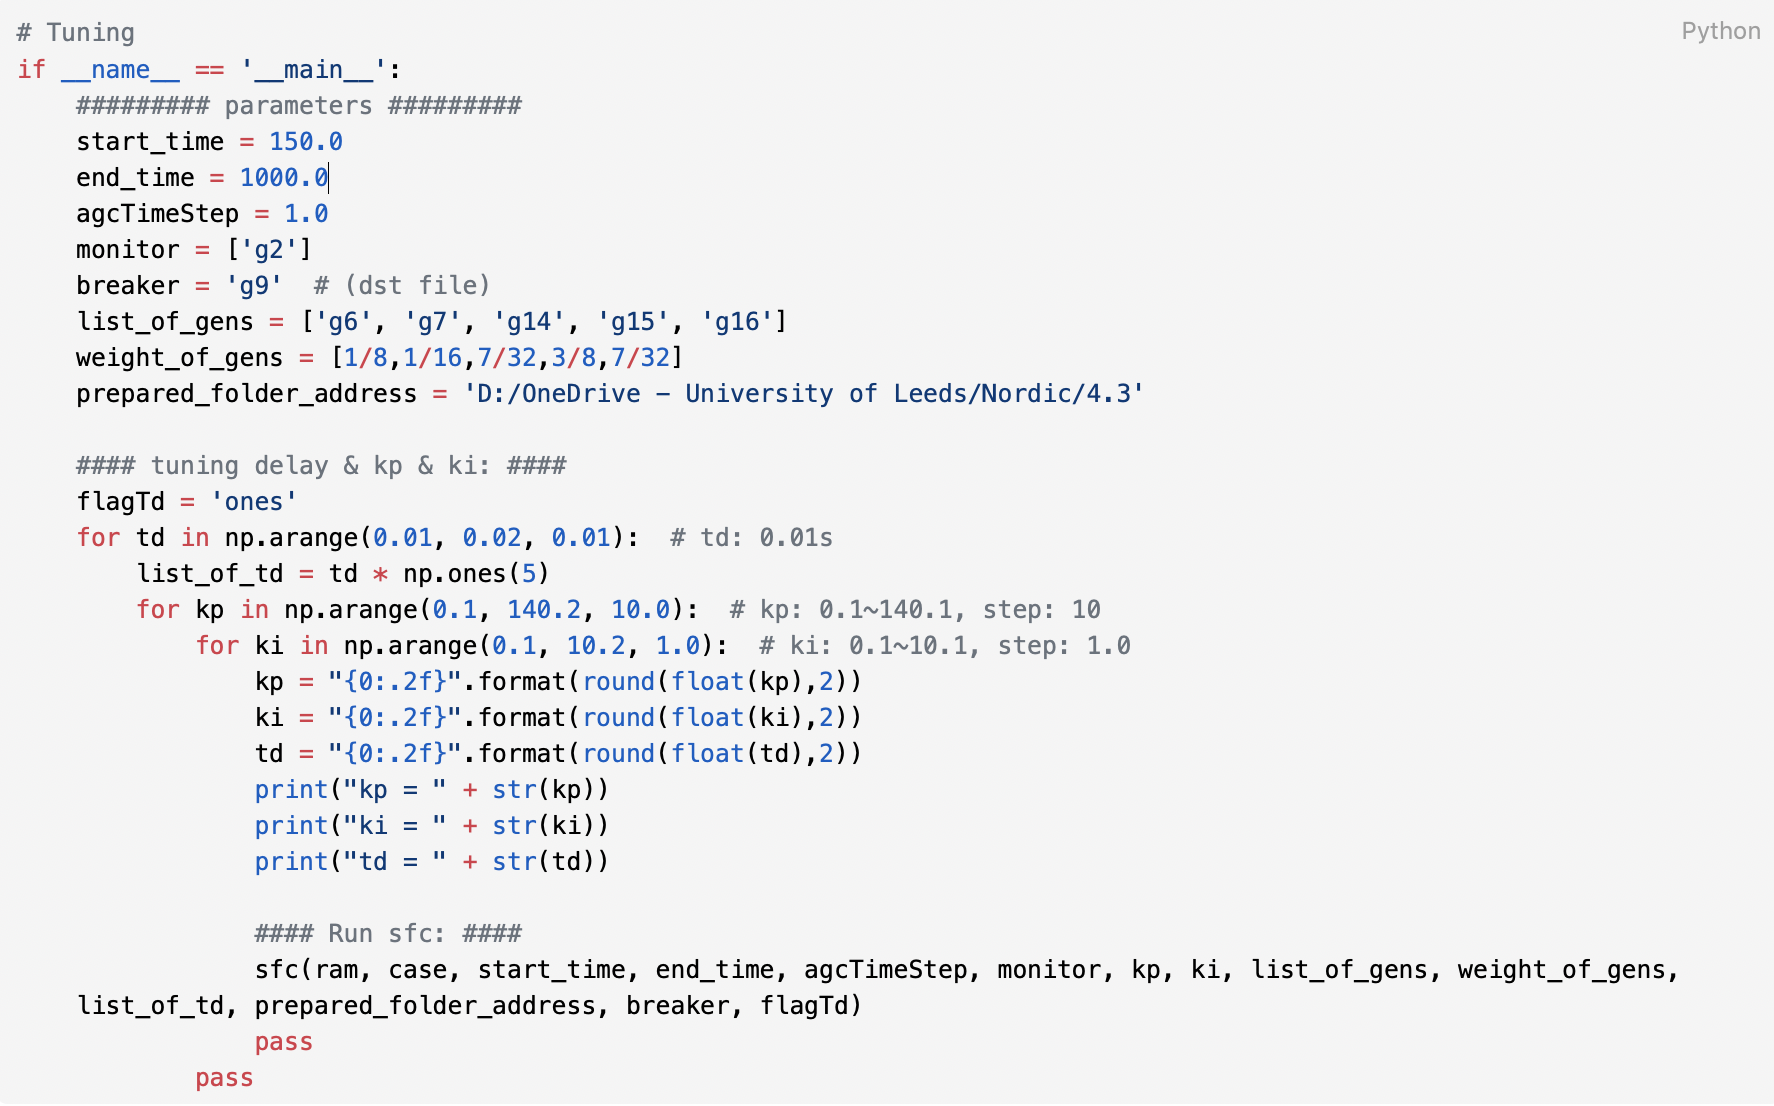
\includegraphics[width = \textwidth]{figure/4_3_code2.png}
%\caption{ }
\label{4_3_code2}
\end{figure}


\section{Results} %4.4
\subsection{Results and Analysis}
The implement results are as follows. Figure \textcolor{red}{\ref{4_4_1_result1}} shows all the acceptable signals.

\begin{figure}[htbp]
\centering
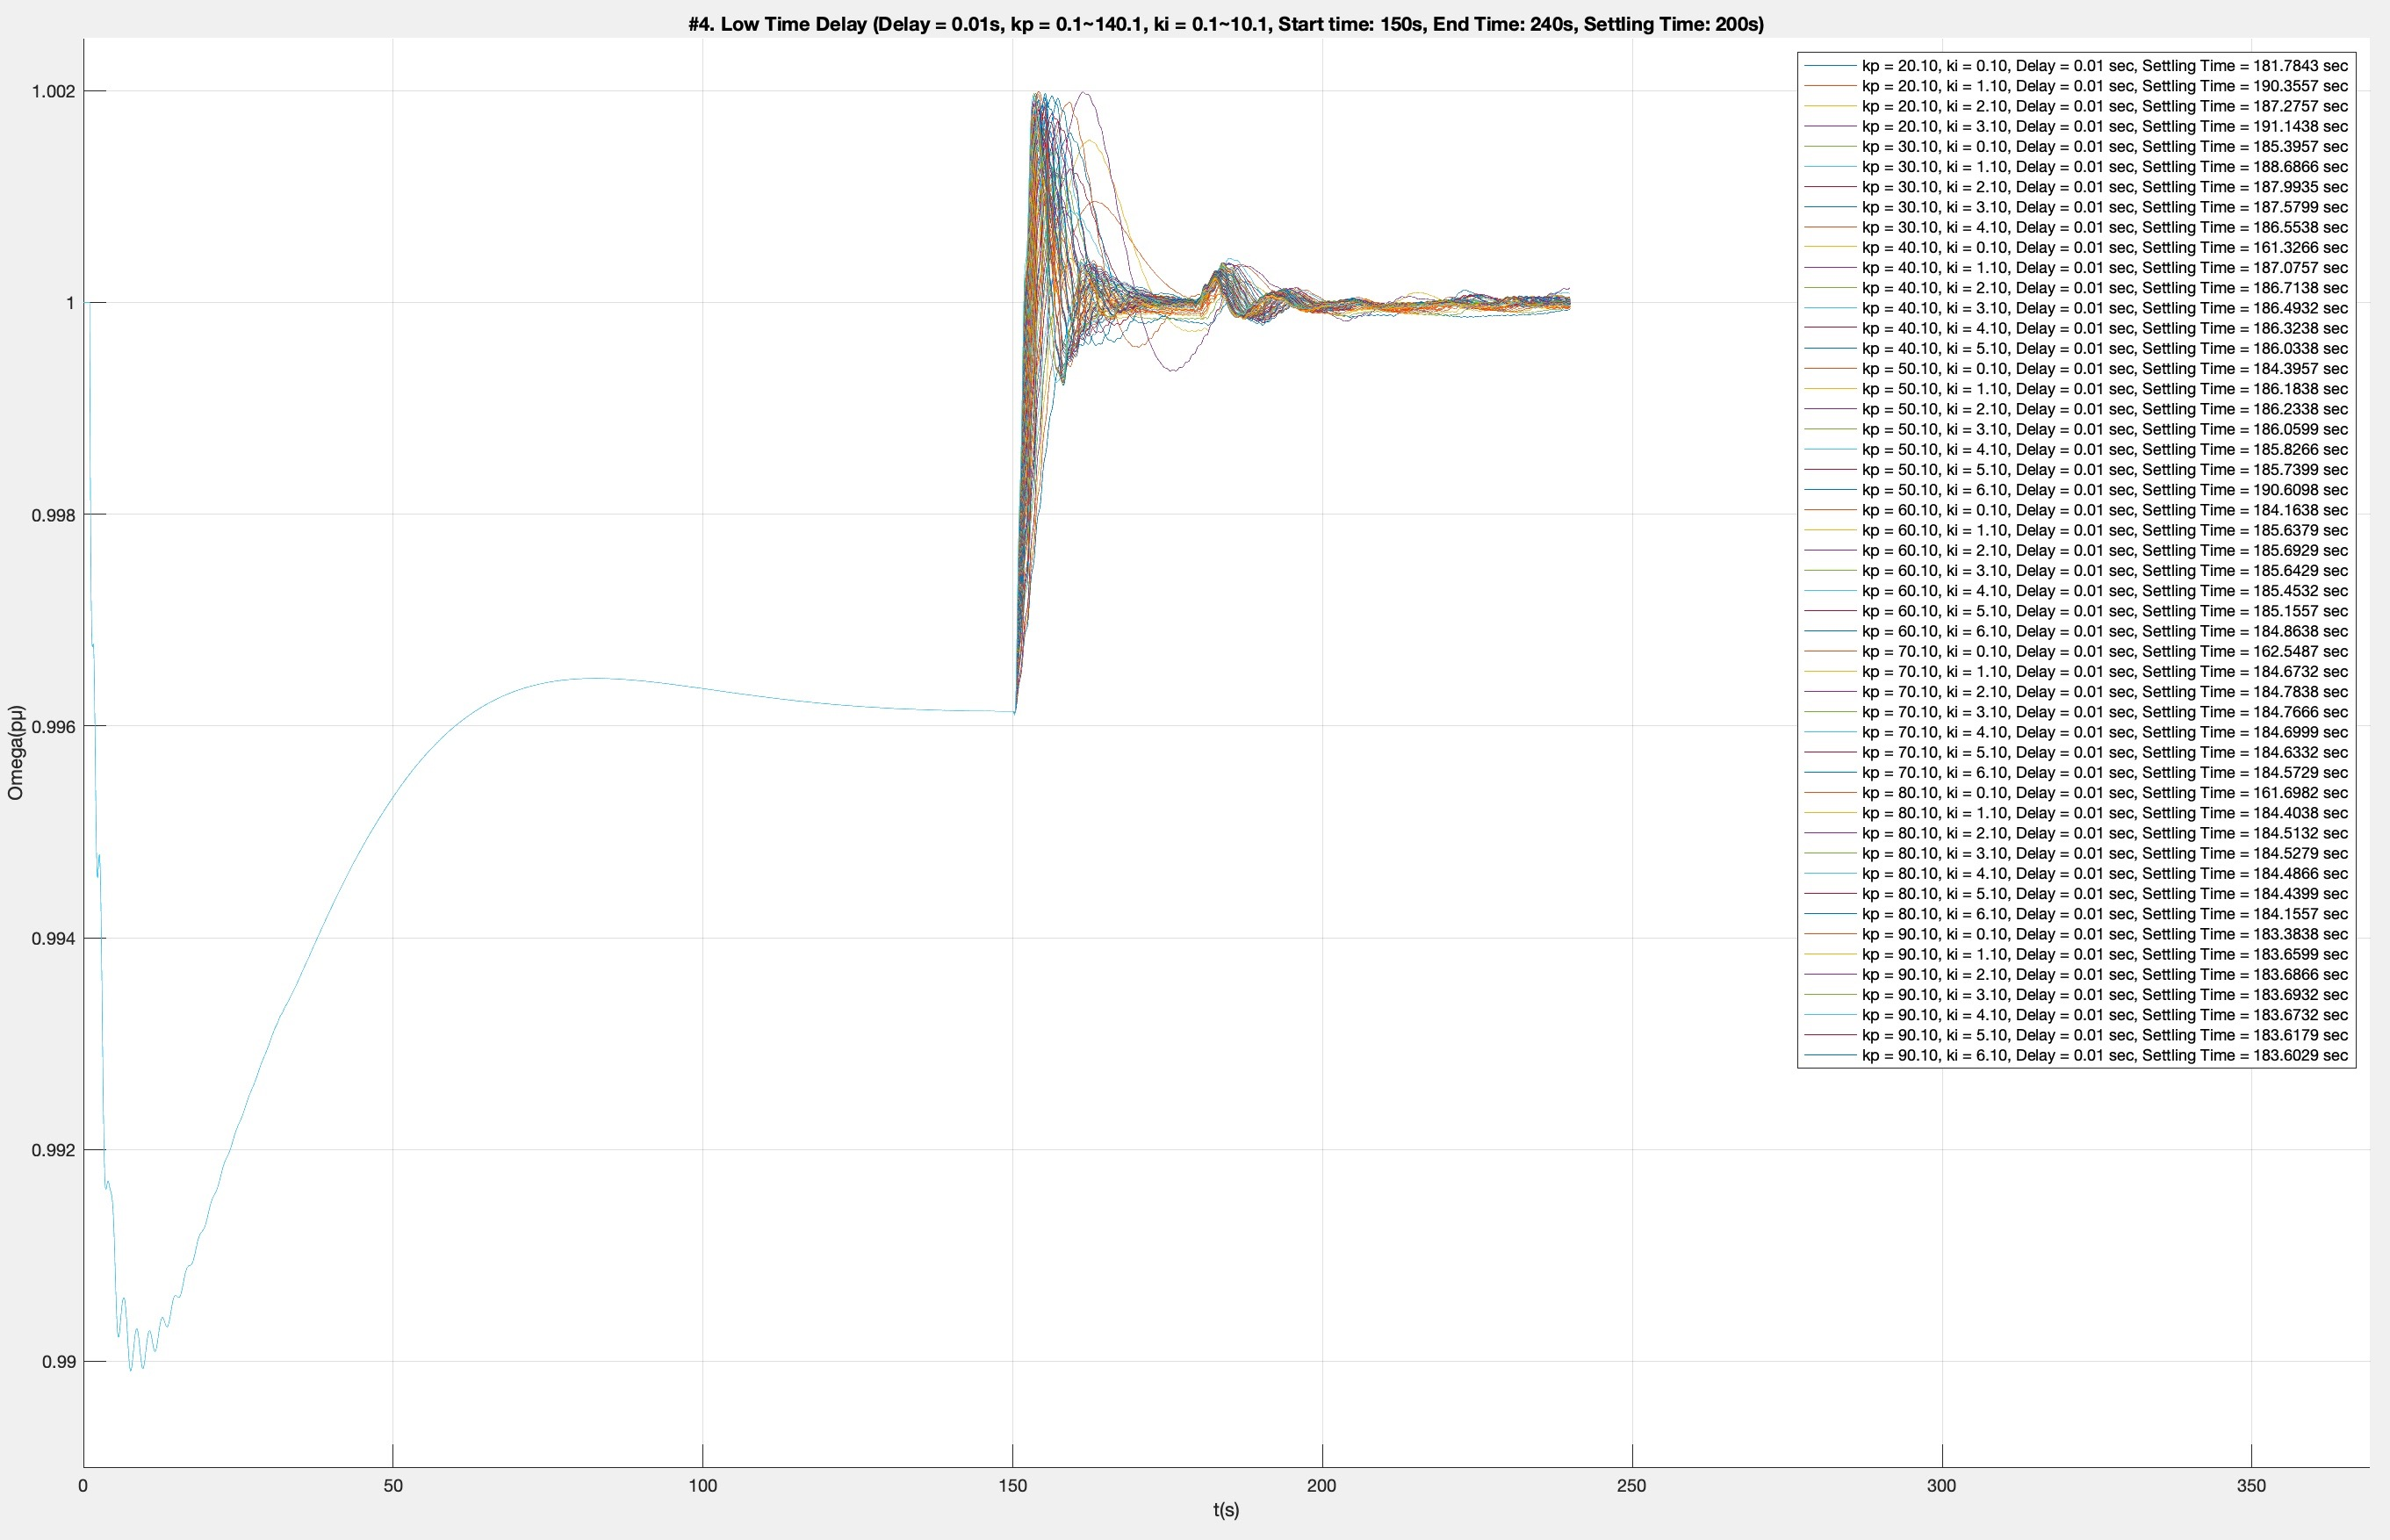
\includegraphics[width = \textwidth]{figure/4_4_1_result1.jpeg}
\caption{}
\label{4_4_1_result1}
\end{figure}

From Figure \textcolor{red}{\ref{4_4_1_result1}}, we can roughly draw a conclusion that the signals are indeed within a reasonable range and it seems that they have finally reached the nominal value. \\

However, we need to check further by choosing one of the signals. For instance, I choose the signal when its kp is 90.1 and its ki is 7.1. The reason I choose this signal is that it is located on the borderline. Results are as follows. \\

\begin{figure}[htbp]
\centering
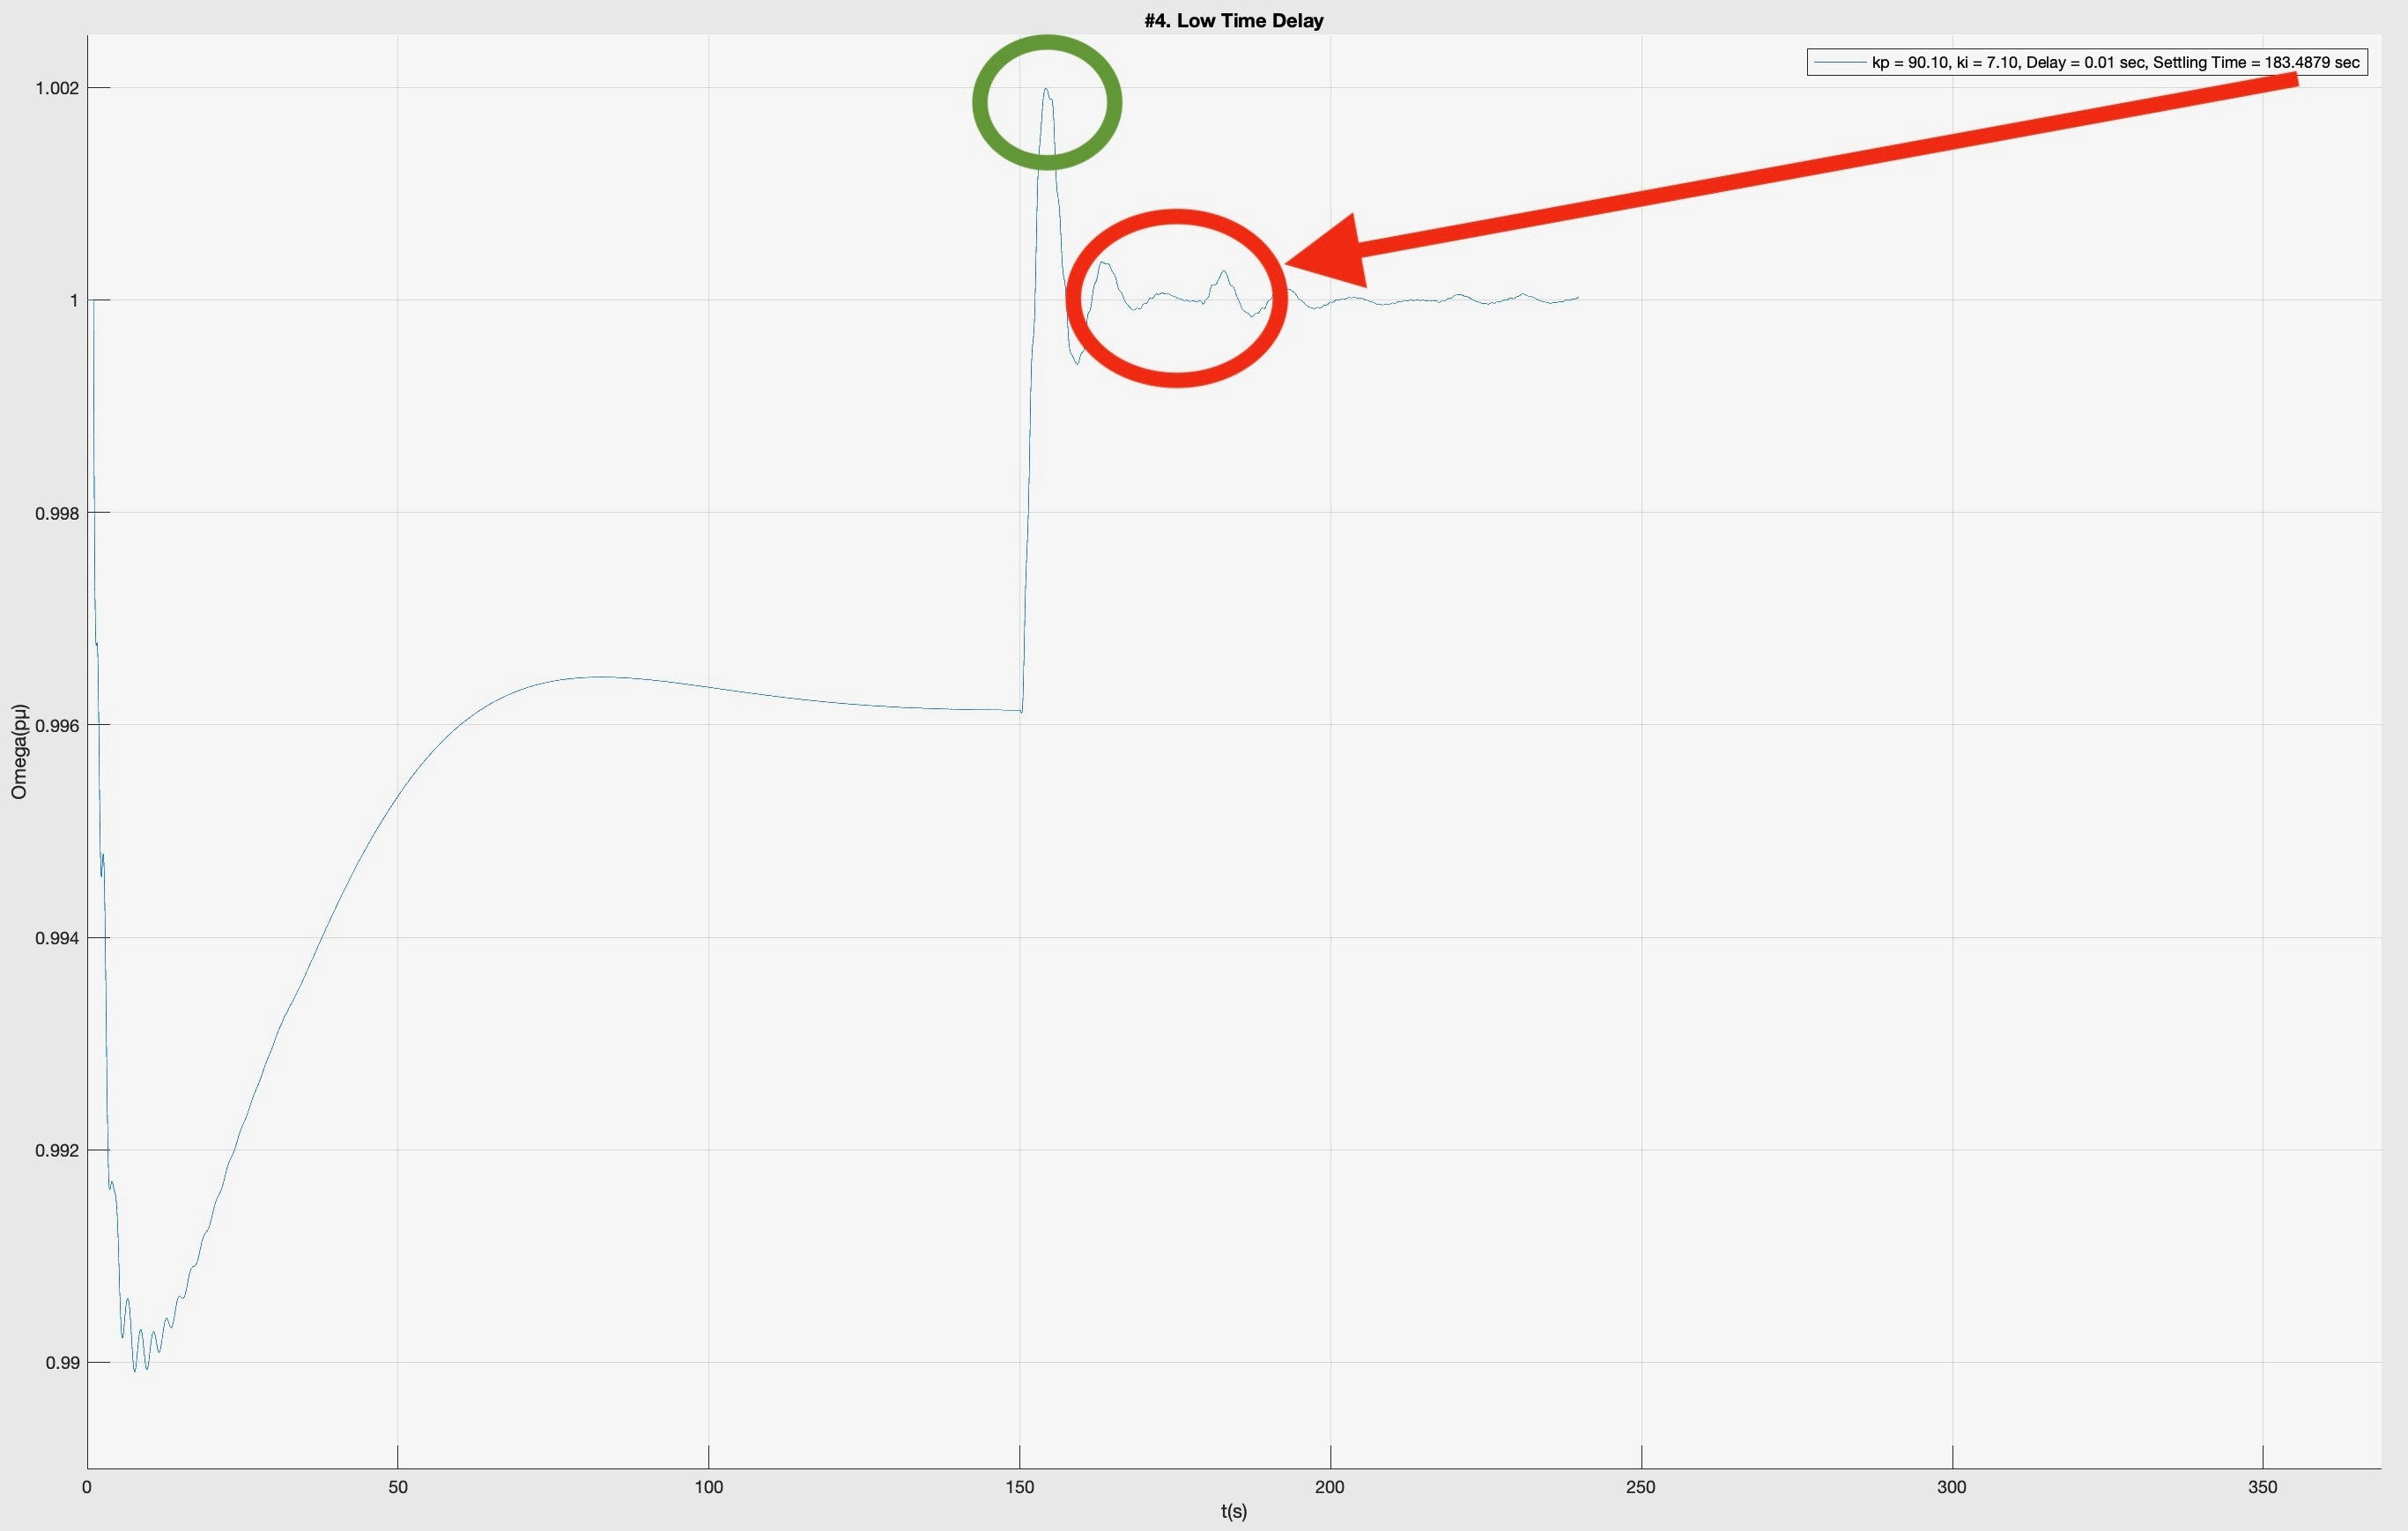
\includegraphics[width = \textwidth]{figure/4_4_1_result2.jpeg}
\caption{}
\label{4_4_1_result2}
\end{figure}

From the Figure \textcolor{red}{\ref{4_4_1_result2}} above, we can see that the overshoot does not exceed 1.002 obviously. But for the settling time, we can not make any conclusion until we see the details. \\


\begin{figure}[htbp]
\centering
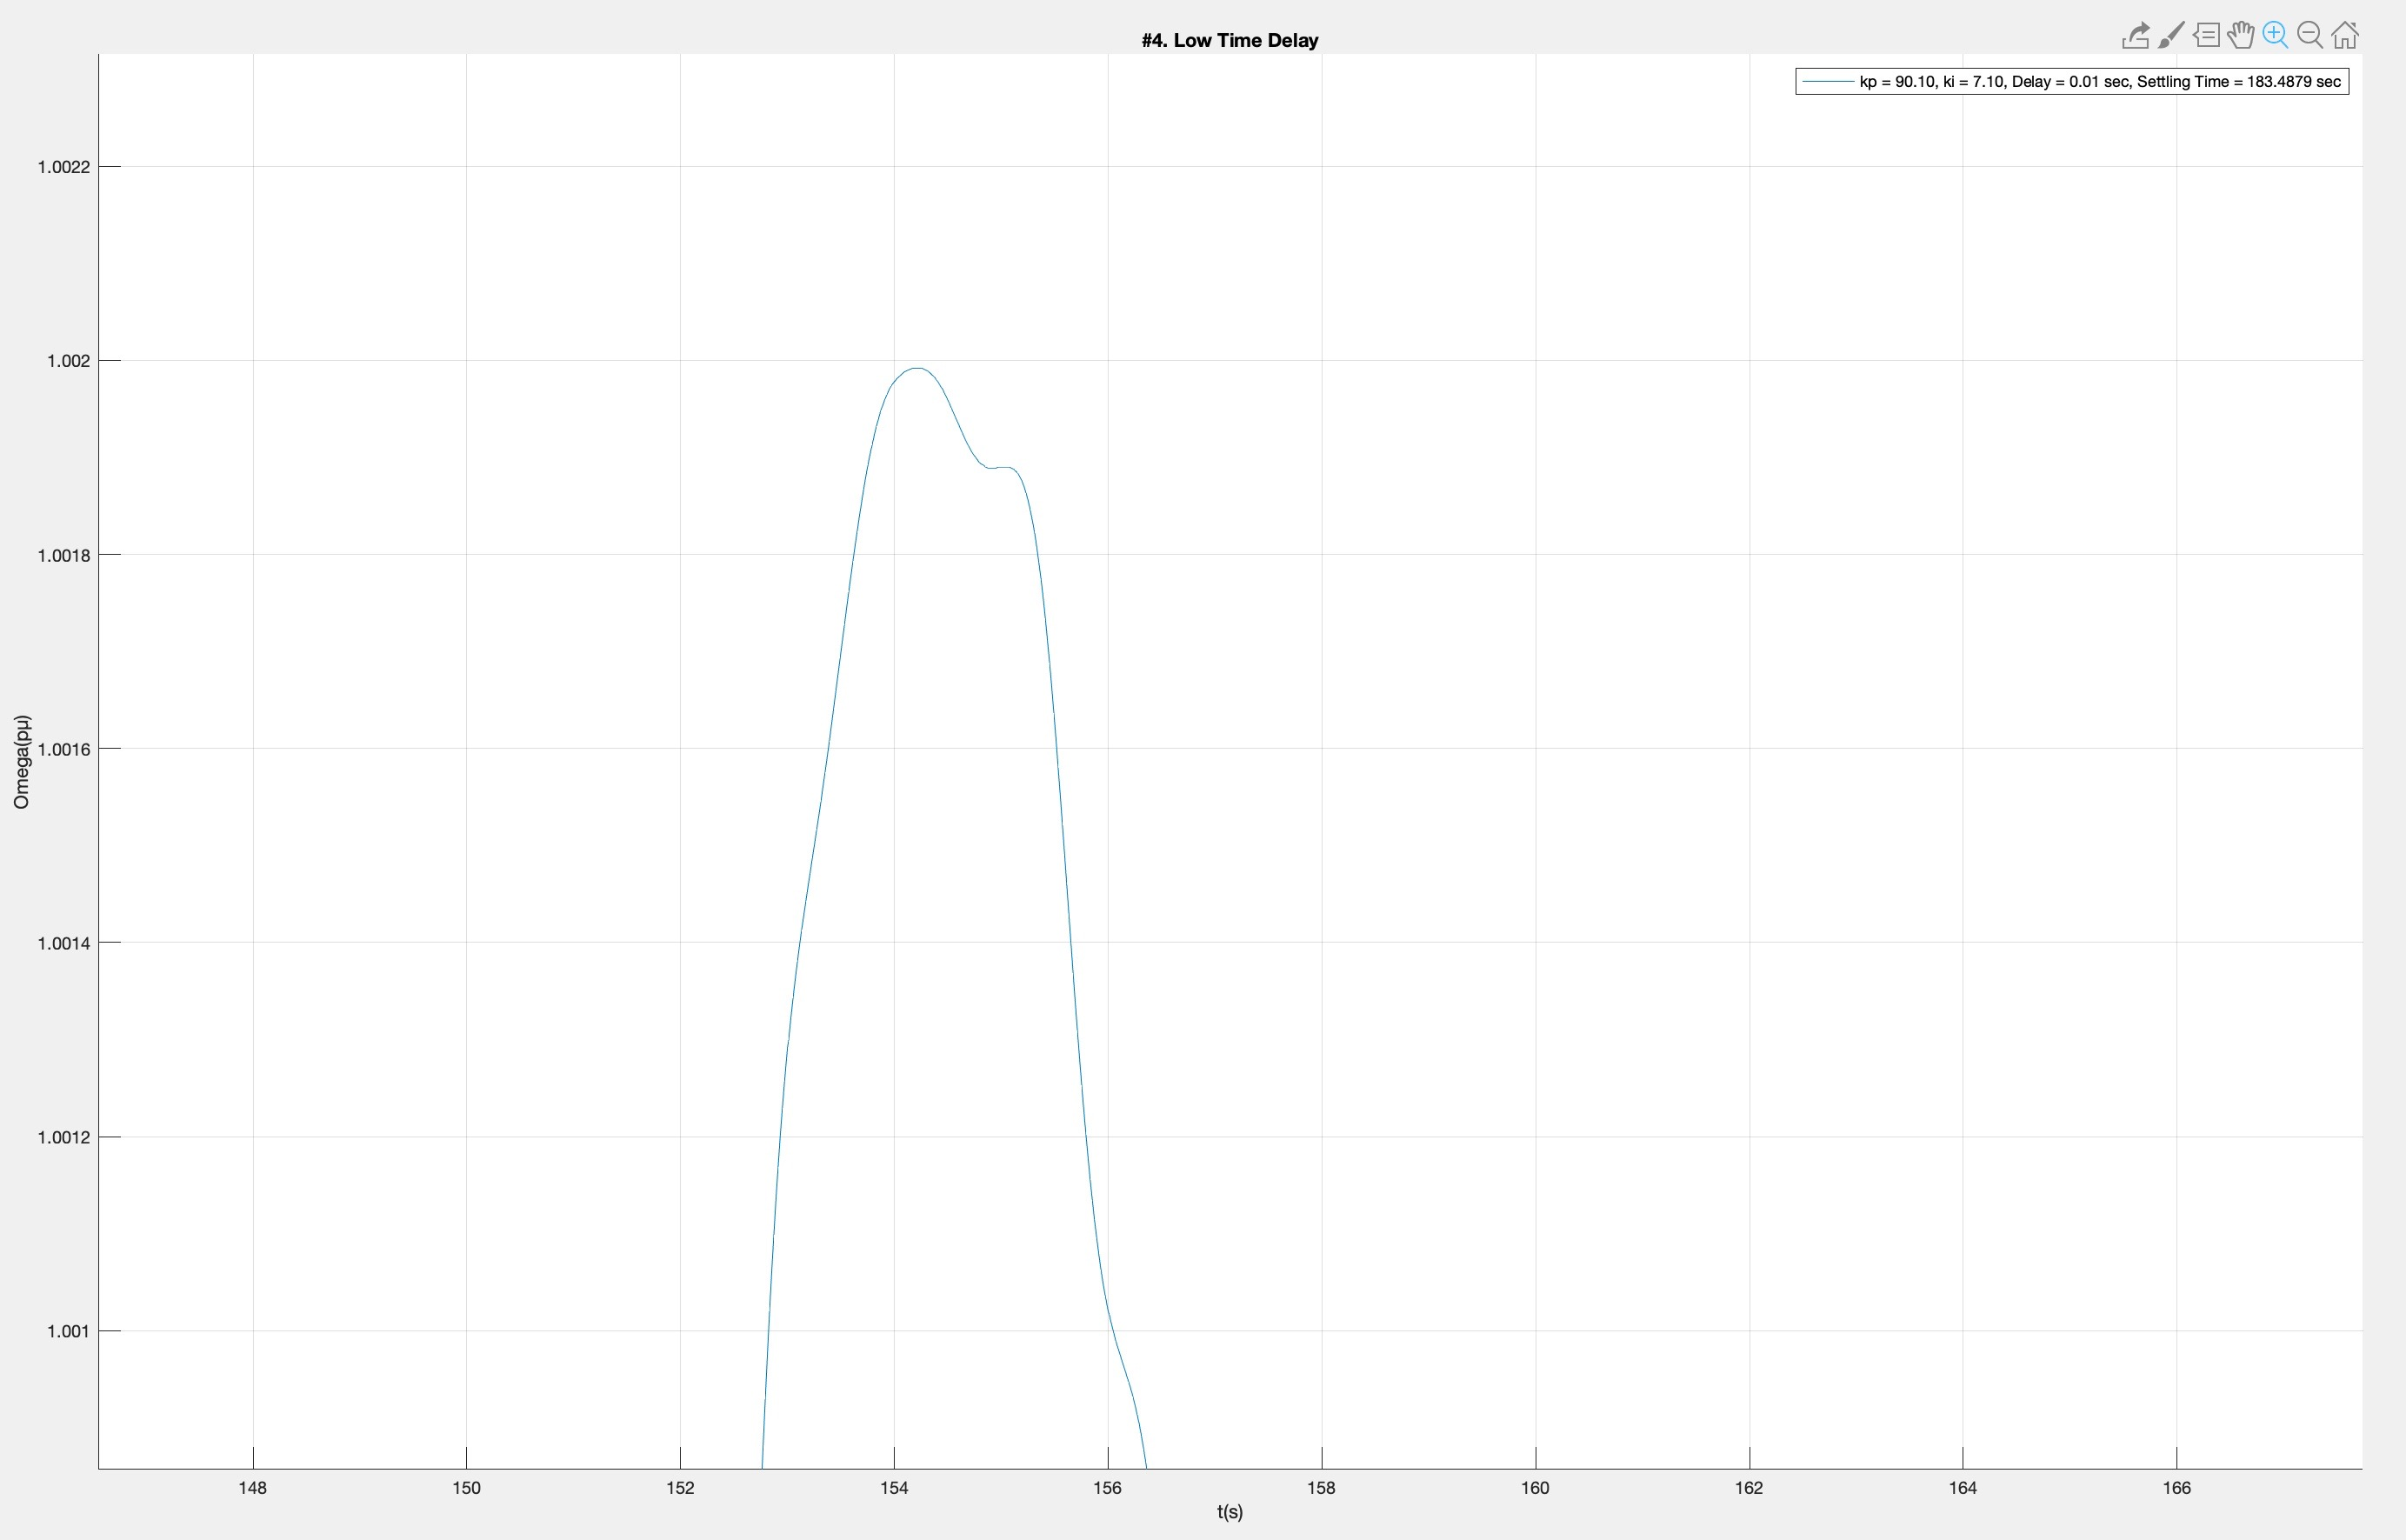
\includegraphics[width = \textwidth]{figure/4_4_1_result3.jpeg}
\caption{}
\label{4_4_1_result3}
\end{figure}

From Figure \textcolor{red}{\ref{4_4_1_result3}}, we can judge its overshoot does do not exceed the maximum allowable value, i.e. 1.002 $p\mu$.

\begin{figure}[htbp]
\centering
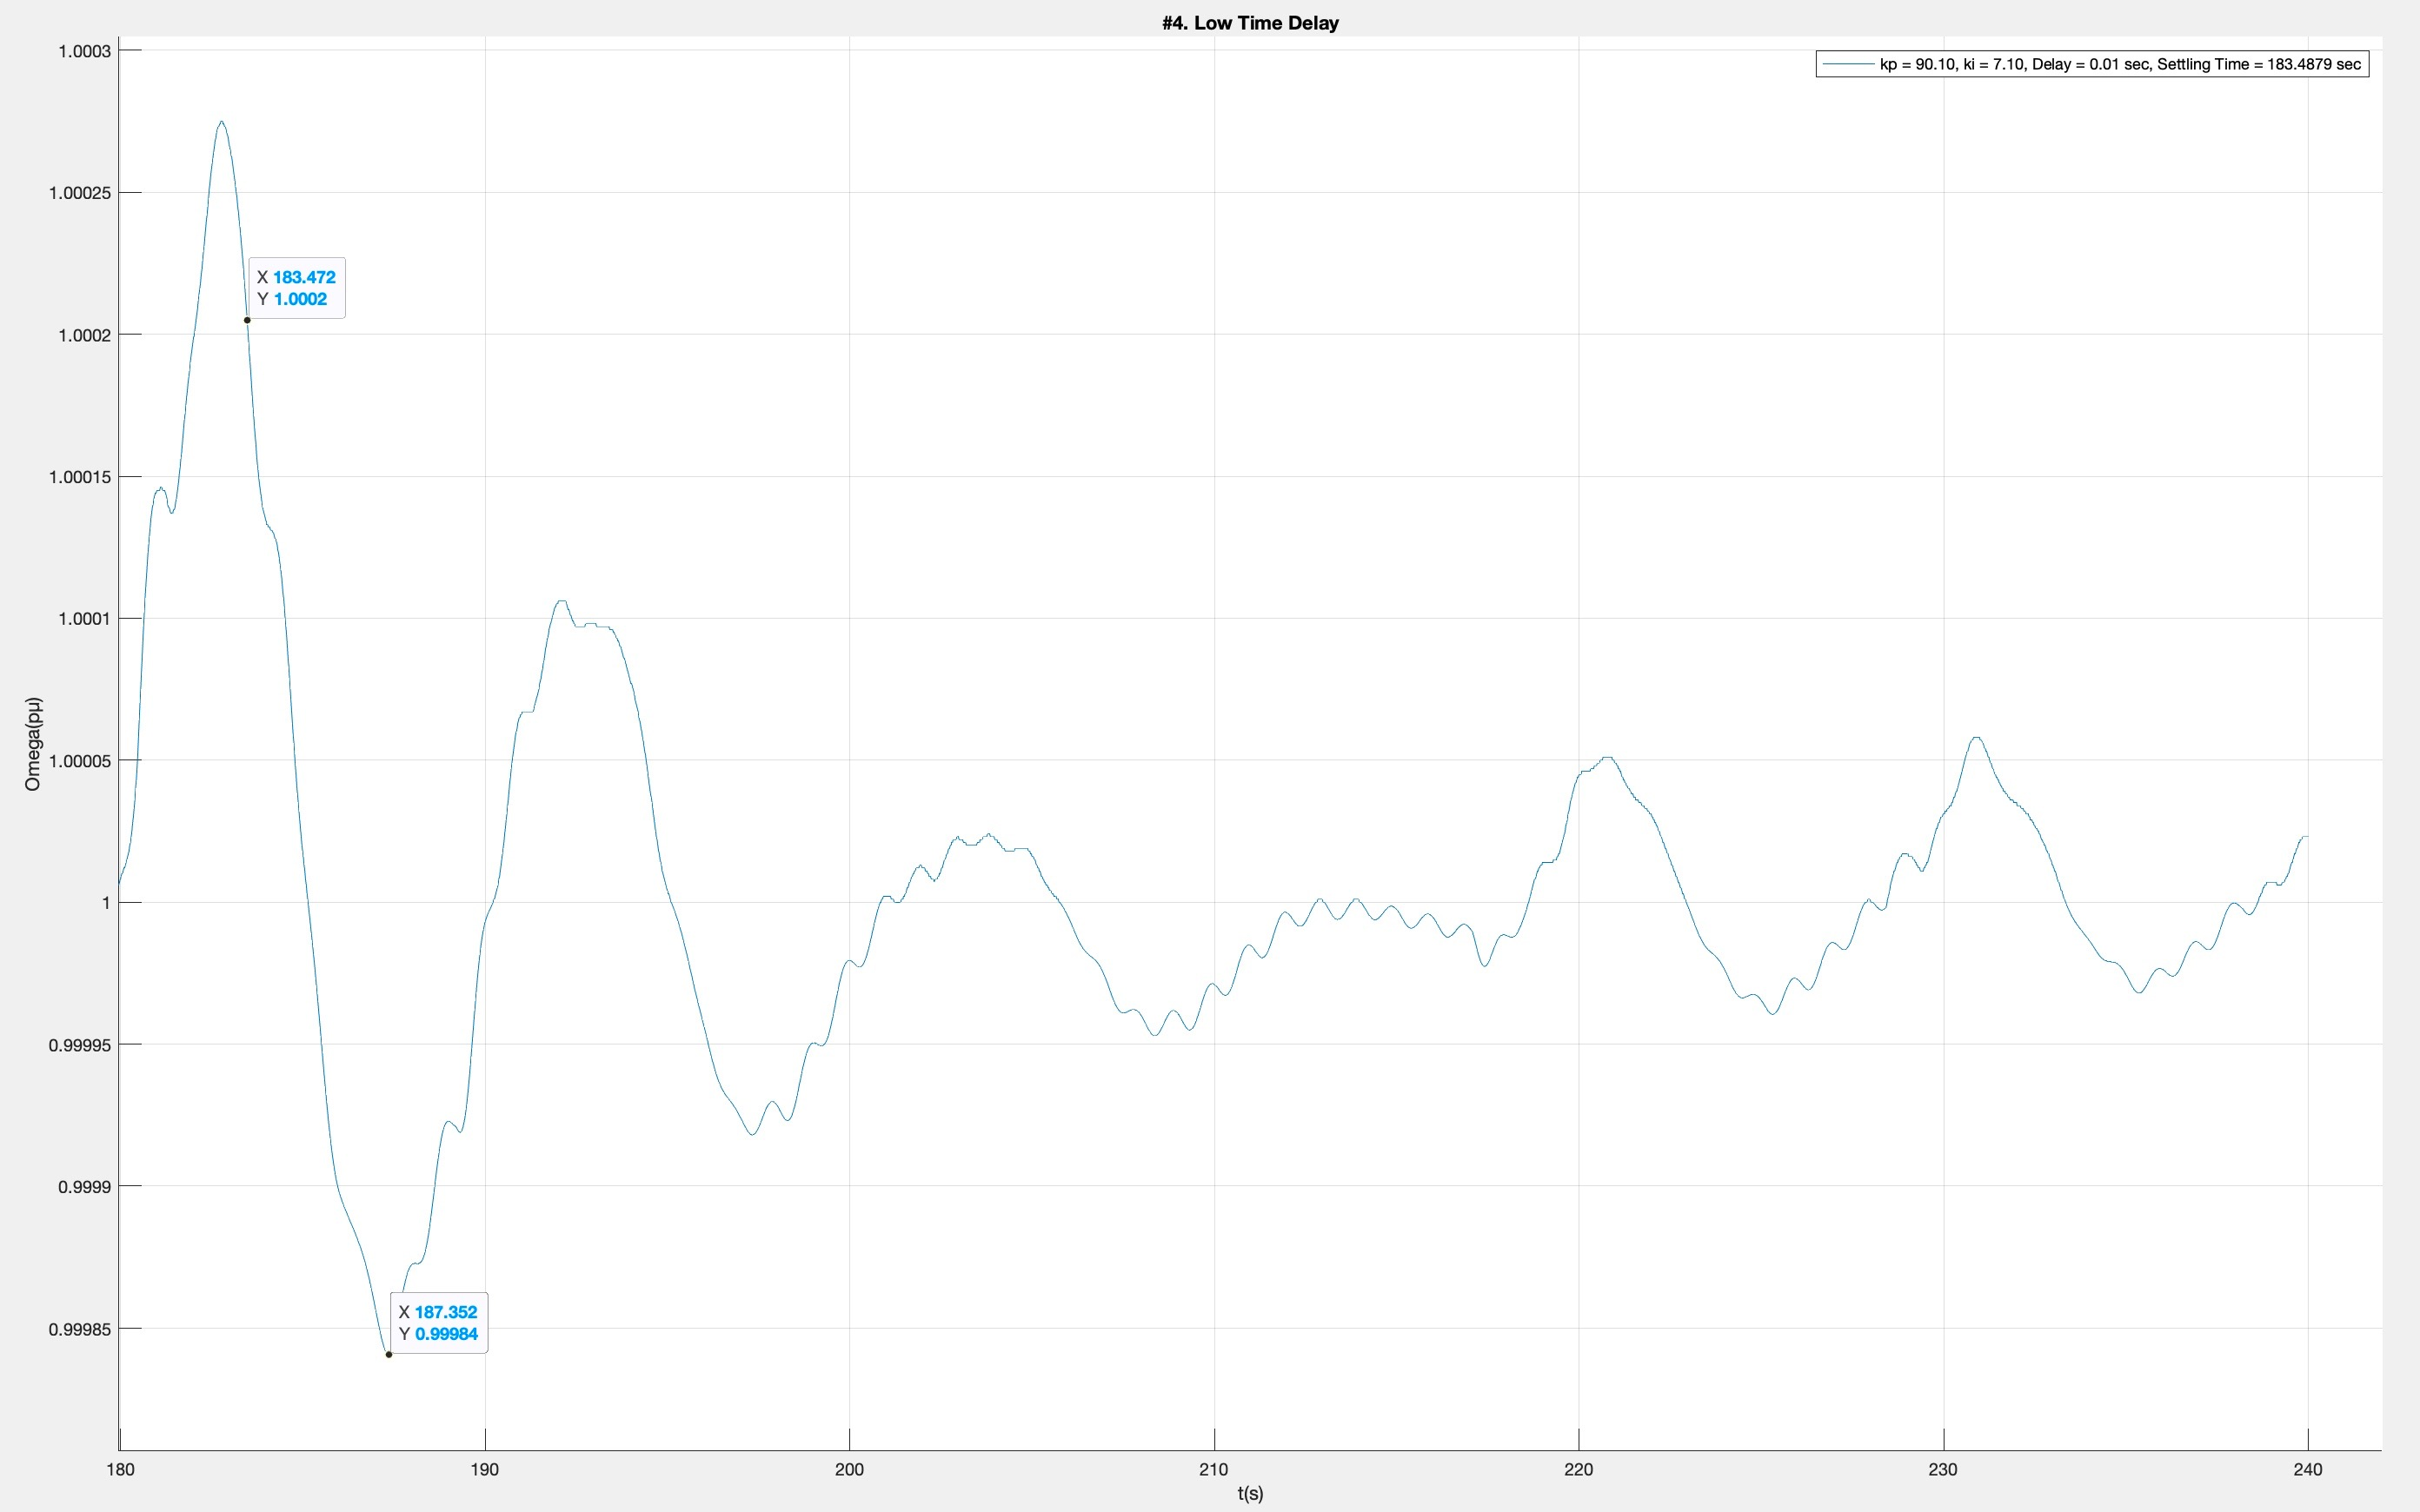
\includegraphics[width = \textwidth]{figure/4_4_1_result4.jpeg}
\caption{}
\label{4_4_1_result4}
\end{figure}


From Figure \textcolor{red}{\ref{4_4_1_result4}}, we find that, after the settling time MATLAB calculated, the signal is between the settling time threshold, i.e. between 0.9998 $p\mu$ and 1.002 $p\mu$. \\

With the prove above, we can finally judge that our assumed acceptable simulation results are acceptable. \\

Next, we will show you the relationship between kp and ki. \\


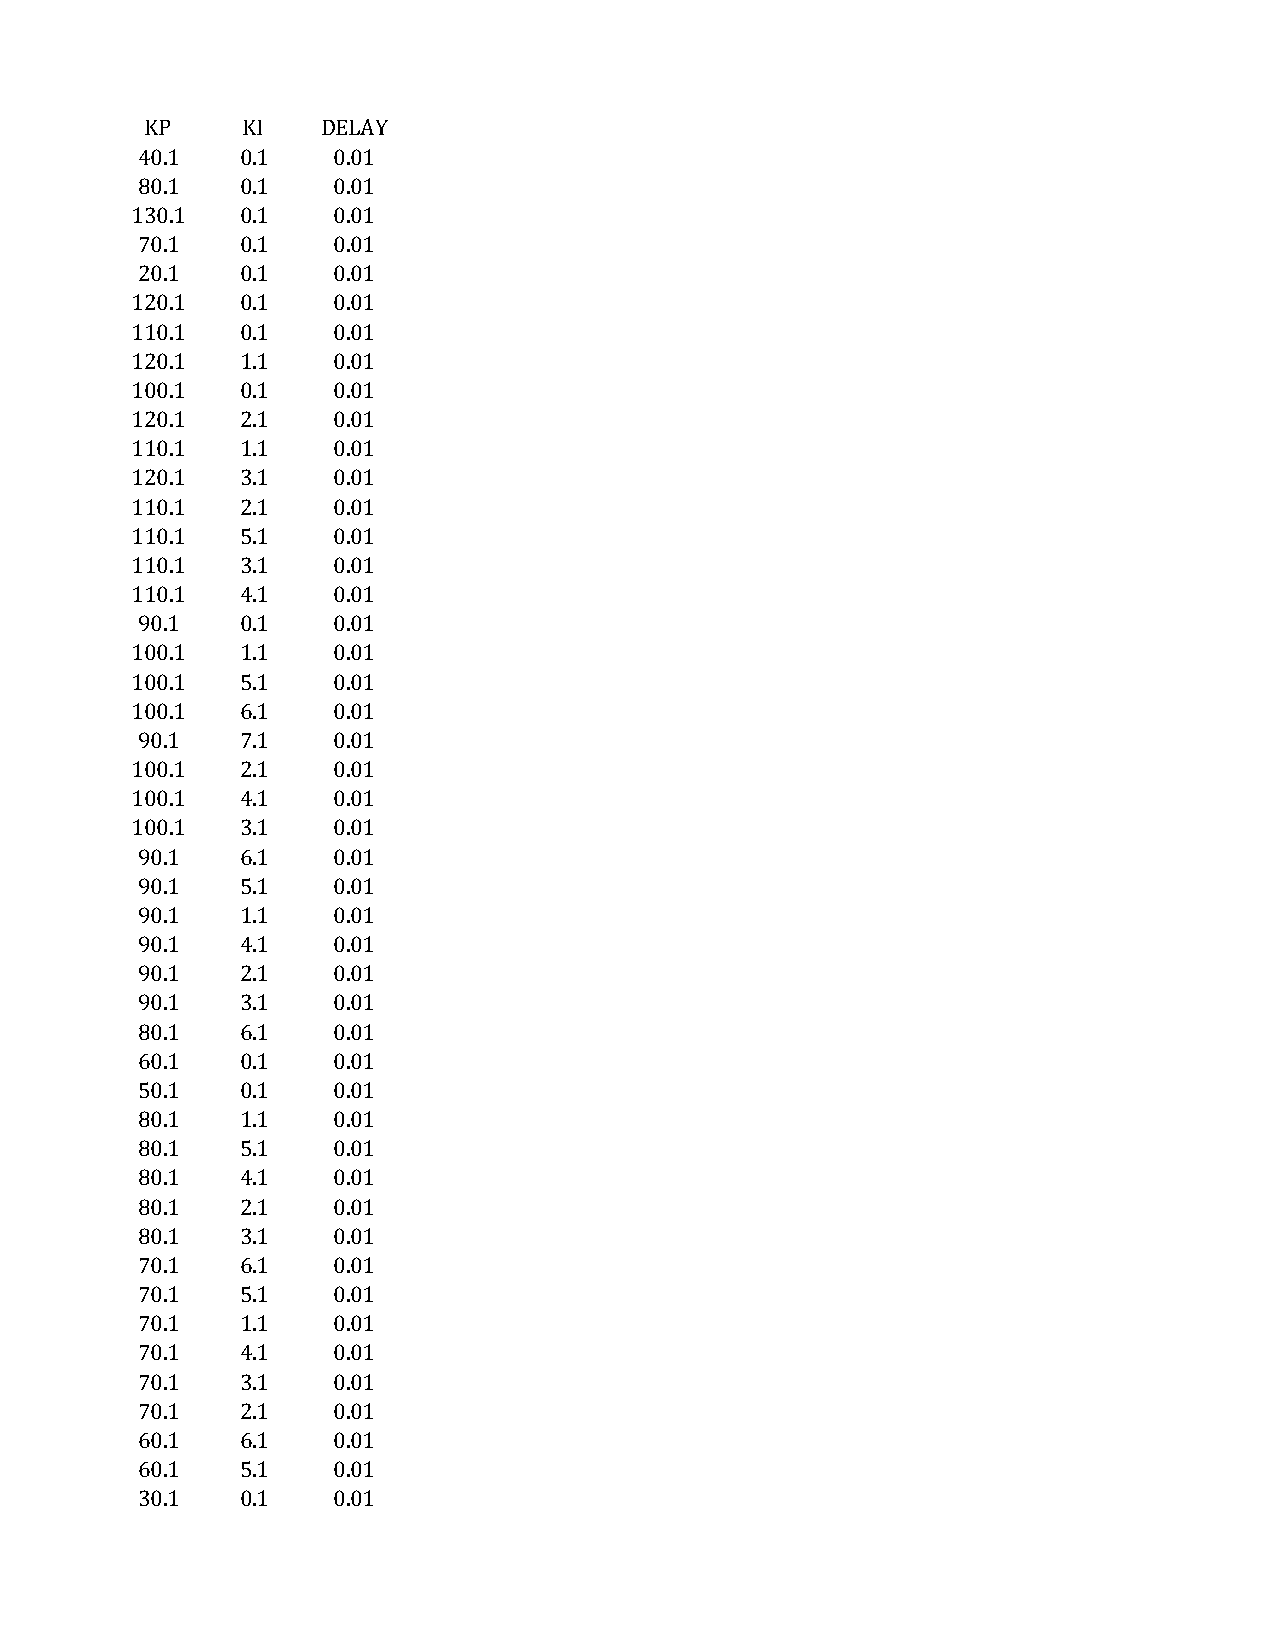
\includepdf[pages=-]{figure/4_4_ori.pdf}
\label{4_4_ori}




 Table \textcolor{red}{\ref{4_4_ori}} shows the parameters that make up the acceptable signals, i.e. kp, ki, delay and settling time. It has ranked by the settling time. 


\begin{figure}[htbp]
\centering
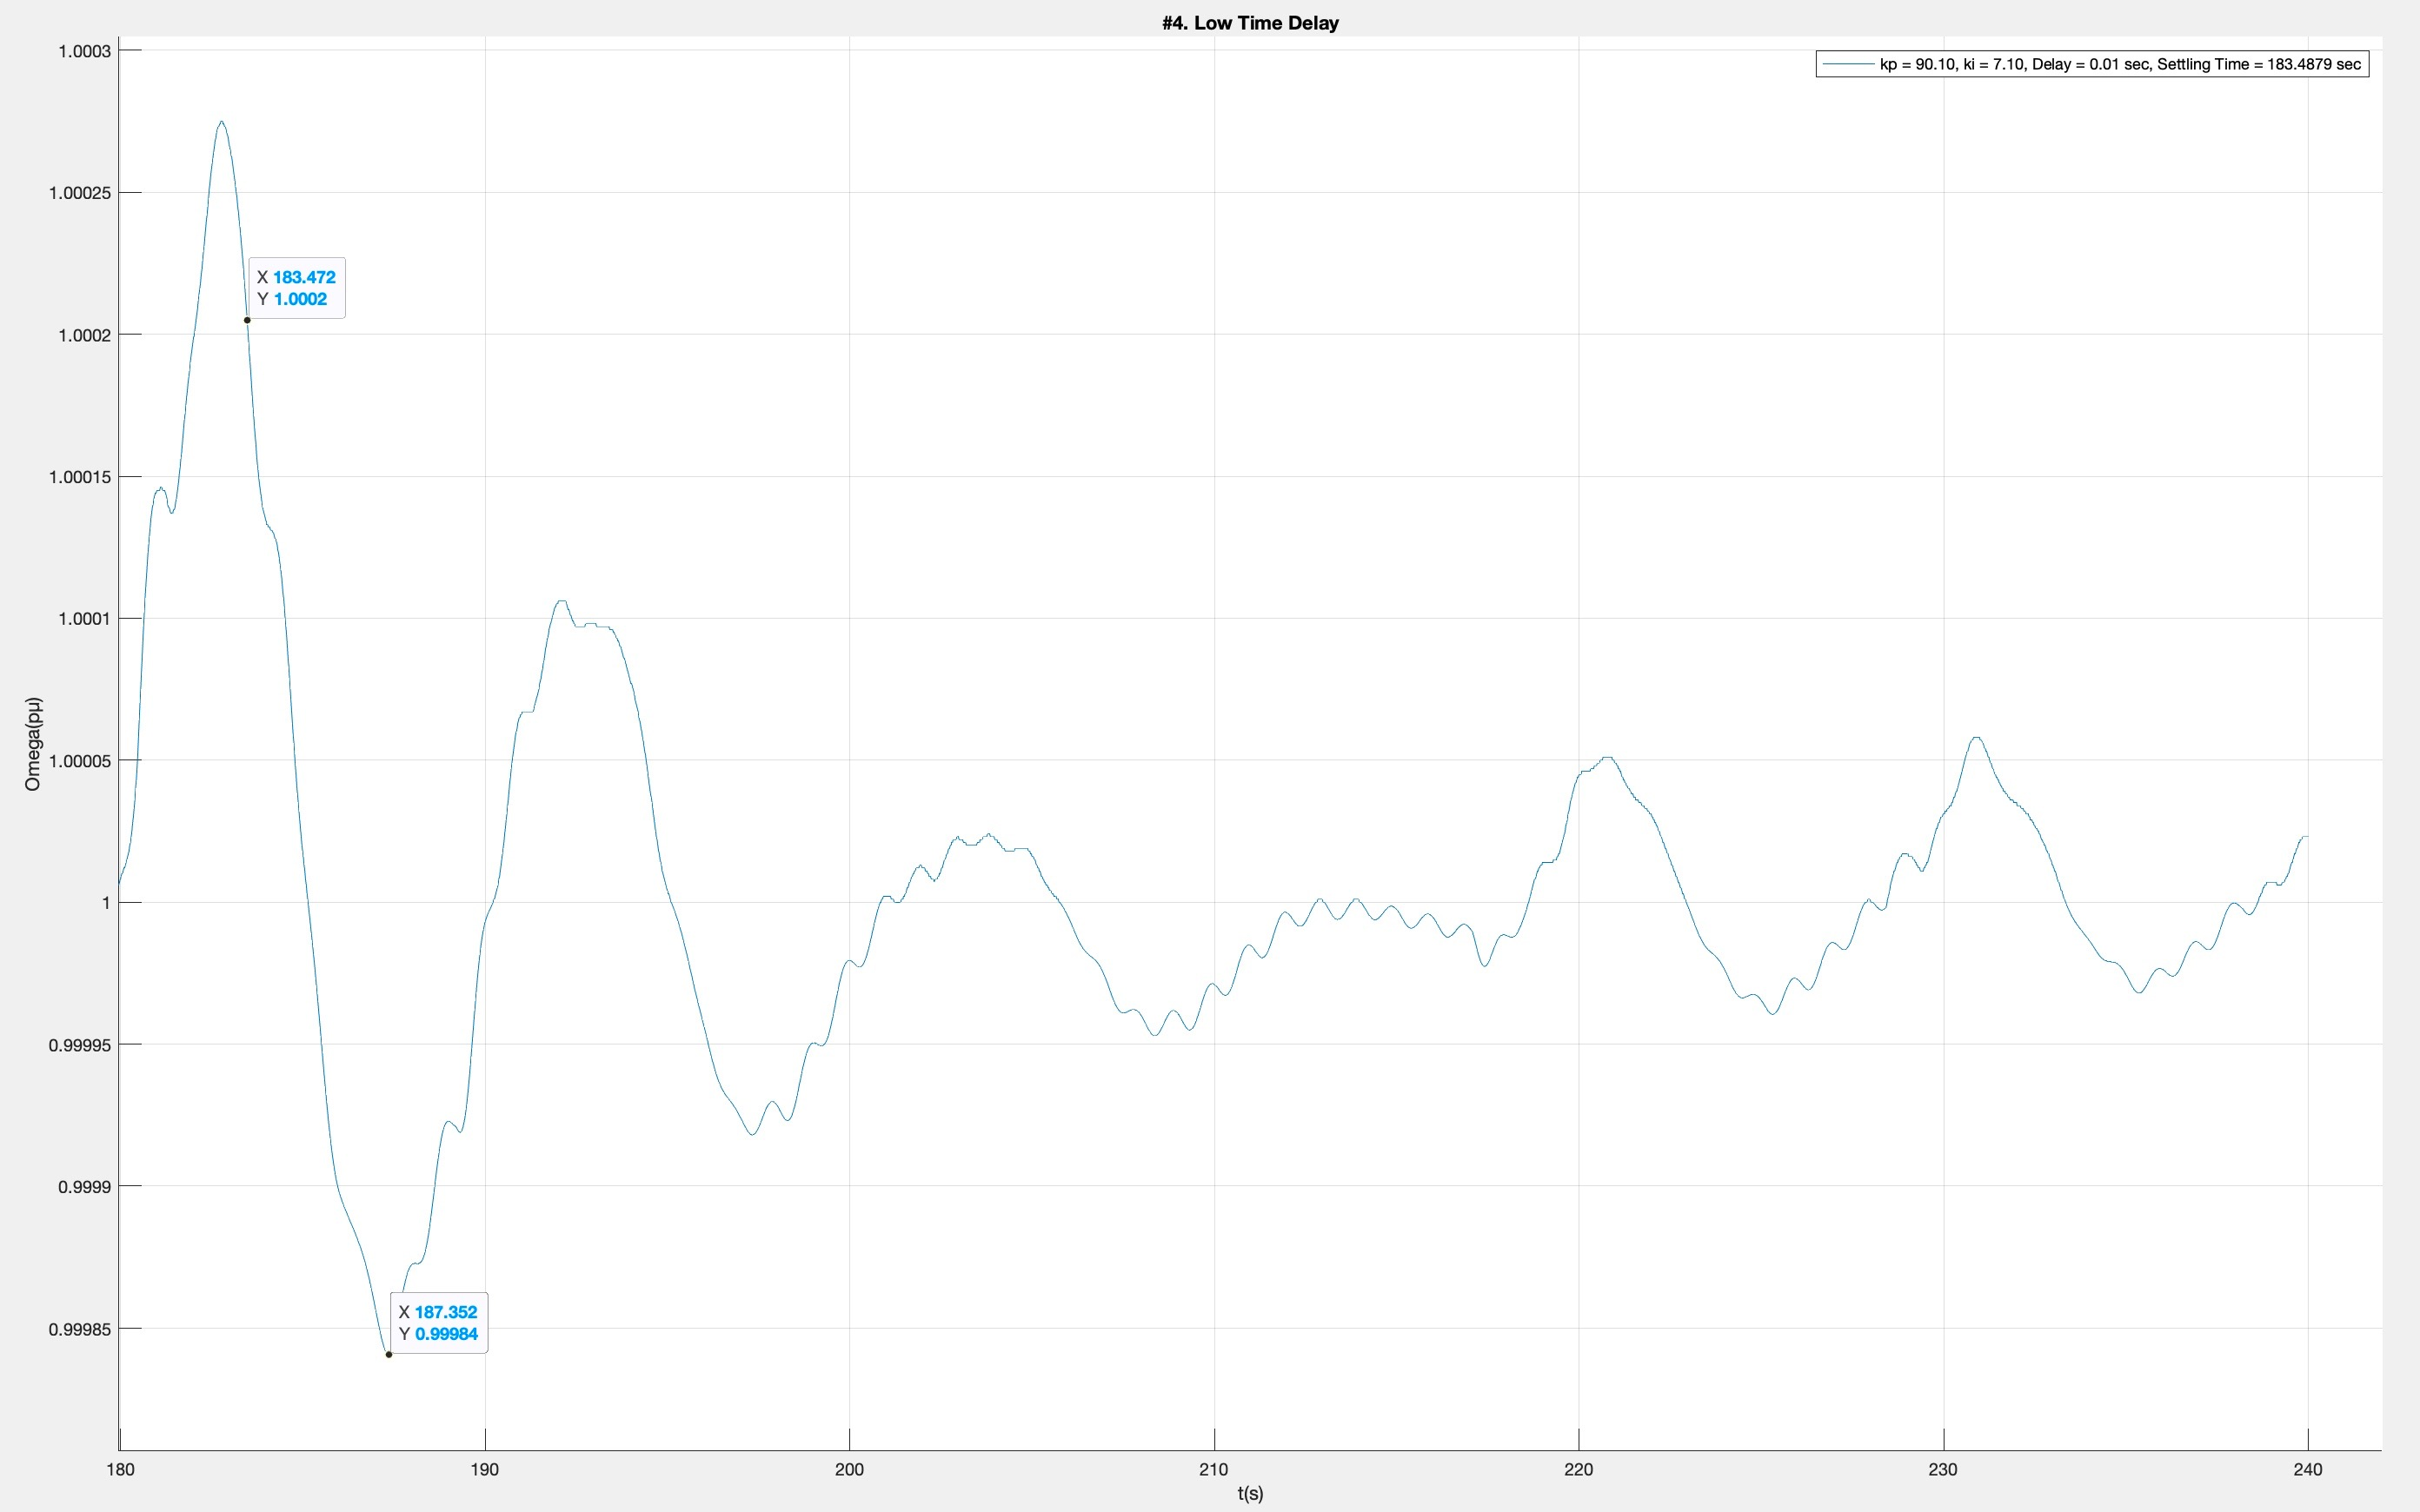
\includegraphics[width = \textwidth]{figure/4_4_1_result4.jpeg}
\caption{}
\label{4_4_1_result4}
\end{figure}











\chapter{Impact of Time Delay}
\label{Chapter5}



\chapter{Impact of Generator Size}
\label{Chapter6}


\chapter{Emergency Control}
\label{Chapter7}


\chapter{Conclusion}
\label{Chapter8}


\appendix
\chapter{}
...
%\bibliographystyle{plain}
%\bibliography{mybib}

\end{document}